%%!TEX encoding = UTF-8 Unicode

% Several lines in file have comments suggesting common packages for the
% typical thesis in informatics or electronics developed at UA
% uncomment/comment the lines as required for your work
% Before each optional line you will have a small comment

% According to UA rules, font size should range from 10 to 12pt.
\documentclass[11pt,a4paper,oneside,onecolumn]{memoir}

\listfiles
%\fixpdflayout

\usepackage[utf8]{inputenc}

% Select Computer Modern Typewritter (For bold ttfamily in listings)
\usepackage{lmodern}
% OR... Bera Mono
%\usepackage[scaled]{beramono} % TTT Font
%\usepackage{anyfontsize} % As the name says...

\usepackage[T1]{fontenc}

% Enable for for Overleaf support
\usepackage{ifthen}
\def\useoverleaf{1}  % change to non-zero (for instance, 1) to enable it

\makeatletter
\newcommand{\makecoverfile}[0]{%
  \immediate\write18{latexmk -pdf cover.tex}%
}
\makeatother

% For PDF merging
\usepackage{pdfpages}

% Set DPI to 300
\pdfpxdimen=\dimexpr 1in/300\relax

% Allow the use of a larger number of packages
\usepackage{morewrites} 

% For English and Portuguese languages
% Portuguese will be the default.
% Uncomment \setlanguage below to change it
\usepackage[english,portuguese]{babel}

% Uncomment to use a custom date format
%\usepackage{datetime}
%\newdateformat{thesisdate}{\monthname[\THEMONTH] \THEYEAR} % Month Year

% Make pdf look better
\usepackage{microtype} 

% Uncomment to enable floats on facing pages
%\usepackage{dpfloat}

% Side by side figures
% Eg. Fig 1a, Fig 1b
\usepackage[hang,small,bf]{caption}
%\let\tion\undefined
%\let\subfloat\undefined
\usepackage{subcaption}

%\RequirePackage{textcase}

% Dropped Caps
%\usepackage{lettrine}

% Configure Hyperlink color
% As a matter or style, you may use this to enable/disable color boxes on links
% \usepackage[breaklinks=true,colorlinks=false,linkcolor=blue]{hyperref}
% Or use the default values provided by the hyperref package
\usepackage[hidelinks]{hyperref}

% Redefine section names according to your preference
%\def\sectionautorefname{Section}
%\def\chapterautorefname{Chapter}
%\def\figureautorefname{Figure}
%\def\listingautorefname{Listing}
%\def\tableautorefname{Table}

% Redefine code boxes
\ifthenelse{\equal{\useoverleaf}{0}}
{\usepackage[outputdir=build]{minted}}
{\usepackage{minted}}%

\addto\captionsportuguese{%
  \renewcommand\listingscaption{Código}
}
\fvset{fontsize=\footnotesize} % Make Code blocks smaller than text
\usepackage{csquotes}

% Add support for PDF Comments
\usepackage{comment}
\ifthenelse{\equal{\useoverleaf}{0}}
{\usepackage{pdfcomment}}{}
\usepackage{bookmark} % New Bookmarks

% For Multiple columns in Glossary
\usepackage{multicol}

% Add support for Math symbols
\usepackage{amsmath}
\usepackage{amssymb}

% Add support for graphics
\usepackage{graphicx}

% Add support for Colors
\usepackage{xcolor}

% Add support for the Euro symbol
\usepackage{eurosym}

% Add support for missingfigure and todo
\usepackage{todonotes}

% Setup bibliography with Biber using IEEE style for proper UTF-8 support
\usepackage[backend=biber, style=ieee, sorting=none, natbib=true, mincitenames=1, maxcitenames=2]{biblatex}
\bibliography{bib/references.bib}

% Use acronyms
\usepackage[printonlyused]{acronym} % For acronyms

% Indenting the first paragraph after section start
\usepackage{indentfirst}

% For fixing listoflistings with memoir
\usepackage{xparse}

% Uncomment the next lines to enable chart support through pgf and tikz
% This may require you to install further packages in your Tex system
%\usepackage[version=0.96]{pgf}
%\usepackage{tikz}

% UML support
%\usepackage{pgf-umlsd}

% Trees, Arrows, Mindmaps and other popular objects
%\usetikzlibrary{arrows,shadows,trees,shapes,decorations,automata,backgrounds,petri,mindmap} % for pgf-umlsd

% Package to master SI units
% \usepackage[detect-weight=true, binary-units=true]{siunitx}
% For Electric Circuits
%\sisetup{load-configurations = binary}

% Set Voltage direction accordingly
% Option : oldvoltagedirection,nooldvoltagedirection,RPvoltages,EFvoltages
% More information at: https://mirrors.ibiblio.org/CTAN/graphics/pgf/contrib/circuitikz/doc/circuitikzmanual.pdf
% By default this template is using the Old Voltage Direction
%\usepackage[oldvoltagedirection,american,cuteinductors,smartlabels]{circuitikz}
%\usetikzlibrary{calc}
%\ctikzset{bipoles/thickness=1}
%\ctikzset{bipoles/length=0.8cm}
%\ctikzset{bipoles/diode/height=.375}
%\ctikzset{bipoles/diode/width=.3}
%\ctikzset{tripoles/thyristor/height=.8}
%\ctikzset{tripoles/thyristor/width=1}
%\ctikzset{bipoles/vsourceam/height/.initial=.7}
%\ctikzset{bipoles/vsourceam/width/.initial=.7}
%\tikzstyle{every node}=[font=\small]
%\tikzstyle{every path}=[line width=0.8pt,line cap=round,line join=round]

% For inline TT text (e.g. code snippets)
\usepackage{verbatim}

% Frames around figures and allow force placement
\usepackage{float}

% Configure Float style
%\floatstyle{boxed}
%\restylefloat{table}
%\restylefloat{figure}
%\restylefloat{lstlisting}

% For test purposes you may use the lipsum package to create dummy text
% \usepackage{lipsum} % REMOVE

%%%%%%%%%%%%%%%%%%%%%%%%%%%%%%%%%%%%%%%%%%%%%%%%%%%
% MY PACKAGES
\usepackage{cellspace}
\usepackage{booktabs}
\usepackage{multirow}
\usepackage{soul}
\usepackage{enumitem}
\usepackage{subcaption}
\usepackage{xcolor}
\usepackage{pgf}
% \usepackage{float}

% Set minimal vertical space above and below the table cells
\setlength\cellspacetoplimit{4pt}
\setlength\cellspacebottomlimit{4pt}

\definecolor{darkgreen}{rgb}{0.0, 0.7, 0.0} 
\definecolor{darkred}{rgb}{0.8, 0.0, 0.0}

\newcommand{\gtext}[1]{%
  \pgfmathsetmacro\pct{round(#1)}%
  \textcolor{darkgreen!\pct!darkred}{\pct\%} %
}


%Keep floats inside section!
\usepackage[section]{placeins}
\let \oldsubsubsection \subsubsection
\renewcommand{\subsubsection}[2][]{
  \FloatBarrier
  \oldsubsubsection#1{#2}
}
\let \oldsubsection \subsection
\renewcommand{\subsection}[2][]{
  \FloatBarrier
  \oldsubsection#1{#2}
}
\let \oldsection \section
\renewcommand{\section}[2][]{
  \FloatBarrier
  \oldsection#1{#2}
}
\let \oldchapter \chapter
\renewcommand{\chapter}[2][]{
  \FloatBarrier
  \oldchapter#1{#2}
}



% Use the built-in division styling
\headstyles{memman}

% Include subsections in the TOC
\settocdepth{subsection}

% Numbering down to subsections as well
\setsecnumdepth{subsection}

% extra index for first lines
\makeindex[lines]

% Margins for University of Aveiro Thesis
\setlrmarginsandblock{3cm}{2.5cm}{*}
\setulmarginsandblock{3cm}{3cm}{*}
\checkandfixthelayout

% Or select your custom spacing to make any ajustment
%\addtolength{\parskip}{0.5\baselineskip}
\linespread{1.5}

\newcommand\mainmatterWithoutReset
{\edef\temppagenumber{\arabic{page}}%
  \mainmatter
  \setcounter{page}{\temppagenumber}%
}

%%%%%%%%%%%%%%%%%%%%%%%%%%%%%%%%%%%%%%%%%%%%%%%%%%
% Document begins here
%%%%%%%%%%%%%%%%%%%%%%%%%%%%%%%%%%%%%%%%%%%%%%%%%%

\begin{document}

% Fix the numbering scheme by having a ghost style for page numbering
\pagenumbering{Alph}

\ifthenelse{\equal{\useoverleaf}{0}}{}{\makecoverfile{}}%
\setcounter{page}{0}\includepdf[pages=-]{cover.pdf}

% Uncomment to enable English
\selectlanguage{english}


% Front matter

%Custom Chapter style named `thesis`
\makechapterstyle{thesis}{% Based on ell
  \chapterstyle{default}
  \renewcommand*{\chapnumfont}{\normalfont\sffamily}
  \renewcommand*{\chaptitlefont}{\normalfont\Huge\sffamily}
  \settowidth{\chapindent}{\chapnumfont 111}
  \renewcommand*{\chapterheadstart}{\begingroup
    \vspace*{\beforechapskip}%
    \begin{adjustwidth}{}{-\chapindent}%
    \hrulefill
    \smash{\rule{0.4pt}{15mm}}
    \end{adjustwidth}\endgroup}
  \renewcommand*{\printchaptername}{}
  \renewcommand*{\chapternamenum}{}
  \renewcommand*{\printchapternum}{%
    \begin{adjustwidth}{}{-\chapindent}
    \hfill
    \raisebox{10mm}[0pt][0pt]{\fontsize{30}{25}\selectfont\chapnumfont \thechapter}%
                              \hspace*{1em}
    \end{adjustwidth}\vspace*{-3.0\onelineskip}}
  \renewcommand*{\printchaptertitle}[1]{%
    \vskip\onelineskip
    \raggedleft {\chaptitlefont ##1}\par\nobreak\vskip 4\onelineskip}}


% Select chapter style from existing or select custom
%\chapterstyle{thesis} % Others: dowding, demo2, dash, chappell, brotherton, bianchi, ger, madsen, tatcher, veelo,indexes)
% thesis can also be used as defined previously
% Check the memoir documentation for the available themes
% Default is veelo
\chapterstyle{veelo}
\makeoddfoot{plain}{}{\thepage}{} % Added by André Zúquete to fix a page numbering issue on the veelo chapter style

% Select Page style
\pagestyle{plain}

% If you feel adventurous you can also define all aspects of your theme
% Use either this input or the chapterstyle before
% % Rules
\newcommand{\thinRule}{\rule{\textwidth}{0.25pt}}

% Customize heading appearances
% Define styles
\newcommand{\partSize}{\Huge}
\newcommand{\partStyle}{\lsstyle\scshape}
\newcommand{\chapterSize}{\Huge}
\newcommand{\chapterStyle}{\lsstyle\scshape}
\newcommand{\chapterAfter}{}
\newcommand{\sectionSize}{\Large}
\newcommand{\sectionStyle}{\scshape\MakeTextLowercase}
\newcommand{\subsectionSize}{\large}
\newcommand{\subsectionStyle}{\scshape\MakeTextLowercase}
\newcommand{\subsubsectionSize}{\large}
\newcommand{\subsubsectionStyle}{\scshape\MakeTextLowercase}
\newlength{\partNumSizePt}
\setlength{\partNumSizePt}{60pt}
\newlength{\chapterNumSizePt}
\setlength{\chapterNumSizePt}{60pt}
\newcommand{\partNumSize}{%
  \fontsize{\partNumSizePt}{1.2\partNumSizePt}\selectfont%
}
\newcommand{\partNumStyle}{\partChapterNumColor}
\newcommand{\chapterNumSize}{%
  \fontsize{\chapterNumSizePt}{1.2\chapterNumSizePt}\selectfont%
}
\newcommand{\chapterNumStyle}{\partChapterNumColor}

% Customize parts
\renewcommand{\partnamefont}{\partSize\partStyle}
\renewcommand{\partnumfont}{\partNumSize\partNumStyle}
\renewcommand{\printpartname}{}
\renewcommand{\printparttitle}[1]{%
  \normalfont\normalcolor\partnamefont #1
}

% Customize chapters
\makeatletter
\setlength{\beforechapskip}{30pt}
\renewcommand*{\chapterheadstart}{\vspace*{\beforechapskip}}
\setlength{\afterchapskip}{3ex}
\setlength{\midchapskip}{3ex}
\renewcommand*{\chapnamefont}{%
  \Large\flushright\chapterStyle\partChapterNumColor%
}
\renewcommand*{\chapnumfont}{\chapterNumSize\chapterNumStyle}
\renewcommand*{\chaptitlefont}{%
  \normalfont\flushleft\normalcolor\chapterSize\chapterStyle%
}
\renewcommand*{\printchaptername}{%
  \chapnamefont\MakeTextLowercase{\@chapapp}%
}
\renewcommand*{\chapternamenum}{\quad}
\renewcommand*{\printchapternum}{%
%  \chapnumfont\textls[-75]{\classicstylenums{\thechapter}}%
 \chapnumfont\textls[-75]{\thechapter}%

}
\renewcommand*{\printchaptertitle}[1]{%
  \chaptitlefont #1
  \chapterAfter
}
\makeatother
% Customize sections and subsections
\setsecnumformat{\csname my#1\endcsname\quad}
\setsecheadstyle{\sectionSize\sectionStyle}
\newcommand{\mysection}{{\thesection}}
\setlength{\beforesecskip}{3em}


\setsubsecheadstyle{\subsectionSize\subsectionStyle}
\newcommand{\mysubsection}{{\normalfont\subsectionSize\thesubsection}}
\setlength{\beforesubsecskip}{3em}

\setsubsubsecheadstyle{\subsubsectionSize\subsubsectionStyle}
\newcommand{\mysubsubsection}{{\normalfont\subsubsectionSize\thesubsubsection}}
\setlength{\beforesubsubsecskip}{2em}

% Customize "Table of ..." appearance
% Customize headings
\newcommand{\renewPrintXTitle}[1]{%
  \renewcommand{#1}[1]{%
    \printchaptertitle{##1}%
  }%
}
\renewPrintXTitle{\printtoctitle}
\renewPrintXTitle{\printlottitle}
\renewPrintXTitle{\printloftitle}

% Customize ToC headings
\renewcommand{\cftpartfont}{\partChapterNumColor\partStyle}
\renewcommand{\cftchapterfont}{\chapterStyle}
\renewcommand{\cftsectionfont}{}
\renewcommand{\cftsubsectionfont}{}
\renewcommand{\cftfigurefont}{}
\renewcommand{\cfttablefont}{}
\newcommand{\cftlstlistingfont}{}

% Increase number width
\newlength{\cftNumWidthIncrease}
\setlength{\cftNumWidthIncrease}{0.25em}
\addtolength{\cftpartnumwidth}{\cftNumWidthIncrease}
\addtolength{\cftchapternumwidth}{\cftNumWidthIncrease}
\addtolength{\cftsectionindent}{\cftNumWidthIncrease}
\addtolength{\cftsubsectionindent}{\cftNumWidthIncrease}
% No leader dots
%\renewcommand*{\cftpartdotsep}{\cftnodots}
%\renewcommand*{\cftchapterdotsep}{\cftnodots}
%\renewcommand*{\cftsectiondotsep}{\cftnodots}
%\renewcommand*{\cftsubsectiondotsep}{\cftnodots}
%\renewcommand*{\cftfiguredotsep}{\cftnodots}
%\renewcommand*{\cfttabledotsep}{\cftnodots}
%\newcommand*{\cftlstlistingdotsep}{\cftnodots}
% Set page numbers immediately after entry text
\newcommand{\tocEntryPageSep}{\hspace{1em}}
\renewcommand{\cftpartleader}{\cftdotfill{\cftdotsep}}
%\renewcommand{\cftpartafterpnum}{\cftparfillskip}
%\renewcommand{\cftchapterleader}{\tocEntryPageSep}
\renewcommand{\cftchapterleader}{\cftdotfill{\cftdotsep}}
%\renewcommand{\cftchapterafterpnum}{\cftparfillskip}
\renewcommand{\cftsectionleader}{\cftdotfill{\cftdotsep}}
%\renewcommand{\cftsectionafterpnum}{\cftparfillskip}
\renewcommand{\cftsubsectionleader}{\cftdotfill{\cftdotsep}}
%\renewcommand{\cftsubsectionafterpnum}{\cftparfillskip}
\renewcommand{\cftfigureleader}{\cftdotfill{\cftdotsep}}
%\renewcommand{\cftfigureafterpnum}{\cftparfillskip}
\renewcommand{\cfttableleader}{\cftdotfill{\cftdotsep}}
%\renewcommand{\cfttableafterpnum}{\cftparfillskip}
\newcommand{\cftlstlistingleader}{\cftdotfill{\cftdotsep}}
%\newcommand{\cftlstlistingafterpnum}{\cftparfillskip}
% Customize page numbers
\newcommand{\tocPageStyle}{\tocPageColor}
\renewcommand{\cftpartpagefont}{\tocPageStyle}
\renewcommand{\cftchapterpagefont}{\tocPageStyle}
\renewcommand{\cftsectionpagefont}{\tocPageStyle}
\renewcommand{\cftsubsectionpagefont}{\tocPageStyle}
\renewcommand{\cftfigurepagefont}{\tocPageStyle}
\renewcommand{\cfttablepagefont}{\tocPageStyle}
\newcommand{\cftlstlistingpagefont}{\tocPageStyle}

% Abstract
% Remove indents around abstract text
\setlength{\absleftindent}{0pt}
\setlength{\absrightindent}{0pt}
% Change font size to conform with the rest of the document text
\renewcommand{\abstracttextfont}{\normalsize}

% Customize headers and footers including page numbers
\newcommand{\hfTextSize}{\footnotesize}
\newcommand{\headTextStyle}{\lsstyle\scshape\MakeTextLowercase}
\nouppercaseheads
\makeevenhead{headings}%
             {\hfTextSize\thepage}%
             {}%
             {\hfTextSize\headTextStyle\leftmark}
\makeevenhead{plain}%
             {\hfTextSize\thepage}%
             {}%
             {\hfTextSize\headTextStyle\leftmark}
\makeoddhead{headings}%
            {\hfTextSize\headTextStyle\rightmark}%
            {}%
            {\hfTextSize\thepage}
\makeoddhead{plain}%
            {\hfTextSize\headTextStyle\rightmark}%
            {}%
            {\hfTextSize\thepage}


% Customize captions
\newcommand{\captionSize}{\small}
\newcommand{\captionStyle}{\scshape}
\newcommand{\captionWidthRatio}{0.9}

\captionnamefont{\captionSize\captionStyle}
\captiontitlefont{\captionSize}
\captiondelim{ -- }
\captiontitlefinal{}
\changecaptionwidth
%\captionwidth{\captionWidthRatio\textwidth}

% Define colors
%\newcommand{\titleColor}{\color[rgb]{0.616, 0.0627, 0.176}}
\newcommand{\titleColor}{\color[rgb]{0,0,0}}

\newcommand{\partChapterNumColor}{\titleColor}
\newcommand{\dropCapColor}{\titleColor}
%\newcommand{\tocPageColor}{\color[rgb]{0.0980, 0.329, 0.651}}

\newcommand{\tocPageColor}{\color[rgb]{0, 0,0}}
\definecolor{shade0}{rgb}{1.0 , 1.0 , 1.0 }
\definecolor{shade1}{rgb}{0.9 , 0.9 , 0.9 }
\definecolor{shade2}{rgb}{0.8 , 0.8 , 0.8 }
\definecolor{shade3}{rgb}{0.65, 0.65, 0.65}
\definecolor{shade4}{rgb}{0.45, 0.45, 0.45}
\definecolor{shade5}{rgb}{0.0 , 0.0 , 0.0 }



%Exclude sub figures from List of Figures
%\captionsetup[subfloat]{list=no}

% Texts
\newenvironment{introduction}
{%
  \begin{minipage}{\textwidth}%
   \itshape%
}
{%
  \end{minipage}%
  \par\addvspace{2\baselineskip plus 0.2\baselineskip minus 0.2\baselineskip}%
}

\frontmatter

\tightlists
\midsloppy
\raggedbottom

\setcounter{tocdepth}{2} %subsections are added to the TOC
\setcounter{secnumdepth}{4} %subsubsections are numbered

% Initial document tables start here: TOC, LOF, LOT, Glossary
% Table of contents with slightly smaller font
{\small\tableofcontents}

% List of figures with slightly smaller font
\clearpage
{\small\listoffigures}

% List of tables with slightly smaller font
\clearpage
{\small\listoftables}

% List of code snippets

% Fix for Listings with memoir

\RenewDocumentCommand \chapter { s O{#3} m }{%
  \FloatBarrier
  \IfValueTF{#1}  % if optional star is seen
    {\oldchapter*{#2}}
    {\oldchapter#1{#2}}
}

%\renewcommand{\listingscaption}{Código}
%\renewcommand{\listoflistingscaption}{Lista de Excertos de Código}
%\clearpage
%{\small\listoflistings}
%\addcontentsline{toc}{chapter}{\listoflistingscaption}

% Reset Chapters
\renewcommand{\chapter}[2][]{
  \FloatBarrier
  \oldchapter#1{#2}
}

% Print Glossary
\clearpage
{\small\chapter{Glossary}

\footnotesize
\SingleSpacing

\begin{multicols}{2}
\begin{acronym}[AAAAAA]

\acro{accs}[ACCS]{Australian Centre for Cyber Security}
\acro{acl}[ACL]{Access Control List}
\acro{ai}[AI]{Artificial Intelligence}
\acro{ann}[ANN]{Artificial Neural Network}
\acro{api}[API]{Application Programming Interface}
\acro{ck}[CK]{Cohen's Kappa}
\acro{cli}[CLI]{Command Line Interface}
\acro{cnn}[CNN]{Convolutional Neural Network}
\acro{cocofl}[CoCoFL]{Communication- and Computation-Aware Federated Learning}
\acro{ddos}[DDoS]{Distributed Denial of Service}
\acro{dl}[DL]{Deep Learning}
\acro{dos}[DoS]{Denial of Service}
\acro{fl}[FL]{Federated Learning}
\acro{fn}[FN]{False Negative}
\acro{fp}[FP]{False Positive}
\acro{gdpr}[GDPR]{General Data Protection Regulation}
\acro{heterofl}[HeteroFL]{Heterogeneous Federated Learning}
\acro{hpc}[HPC]{High-Performance Computing}
\acro{ids}[IDS]{Intrusion Detection System}
\acro{iid}[IID]{Independent and Identically Distributed}
\acro{iot}[IoT]{Internet of Things}
\acro{jsonl}[JSONL]{JavaScript Object Notation Lines}
\acro{mae}[MAE]{Mean Absolute Error}
\acro{mcc}[MCC]{Matthews Correlation Coefficient}
\acro{mitm}[MITM]{Man In The Middle}
\acro{mit}[MIT]{Massachusetts Institute of Technology}
\acro{ml}[ML]{Machine Learning}
\acro{mpi}[MPI]{Message Passing Interface}
\acro{mqtt}[MQTT]{Message Queuing Telemetry Transport}
\acro{mse}[MSE]{Mean Squared Error}
\acro{mtls}[mTLS]{Mutual Transport Layer Security}
\acro{nn}[NN]{Neural Network}
\acro{non-iid}[Non-IID]{Non-Independent and Identically Distributed}
\acro{ntp}[NTP]{Network Time Protocol}
\acro{pi}[PI]{Permutation Importance}
\acro{pypi}[PyPI]{Python Package Index}
\acro{relu}[ReLU]{Rectified Linear Unit}
\acro{rnn}[RNN]{Recurrent Neural Network}
\acro{sae}[SAE]{Sparse AutoEncoder}
\acro{smape}[SMAPE]{Symmetric Mean Absolute Percentage Error}
\acro{ssh}[SSH]{Secure Shell}
\acro{tcp}[TCP]{Transmission Control Protocol}
\acro{tls}[TLS]{Transport Layer Security}
\acro{tn}[TN]{True Negative}
\acro{tp}[TP]{True Positive}
\acro{udp}[UDP]{User Datagram Protocol}
\acro{vm}[VM]{Virtual Machine}
\acro{xai}[XAI]{Explainable Artificial Intelligence}
\acro{xss}[XSS]{Cross-Site Scripting}

\end{acronym}
\end{multicols}

}

%%%%%%%%%%%%%%%%%%%%%%%%%%%%%%%%%%%%%%%%%%%%%%%%%%%%%%%
% Main document starts here
%%%%%%%%%%%%%%%%%%%%%%%%%%%%%%%%%%%%%%%%%%%%%%%%%%%%%%%

\mainmatter

% Line spacing: 1.5 pt 
\OnehalfSpacing


%%%%%%%%%%%%%%%%%%%%%%%%%%%%%%%%%%%%%%%%%%%%%%%%%%%%%%%
% Start of Thesis text 
%%%%%%%%%%%%%%%%%%%%%%%%%%%%%%%%%%%%%%%%%%%%%%%%%%%%%%%

% Uncomment to add further chapters
\chapter{Introduction}
\label{chapter:introduction}

\begin{introduction}

This chapter introduces the growing relevance of Artificial Intelligence and Federated Learning, highlighting the core challenges addressed in this research, specifically concerning resilience and modularity in dynamic, distributed environments.

\end{introduction}


\section{Context}

\ac{ai} is becoming increasingly used in our daily lives, revolutionizing industries ranging from healthcare and finance to transportation and education \cite{rashid2024ai}. This widespread adoption highlights \ac{ai}'s potential to address complex problems, automate processes, and drive innovation. Yet, training \ac{ml} models has significant challenges, especially when dealing with sensitive or distributed data \cite{xu2021privacy}.

\ac{fl} offers a promising approach to resolving these challenges by leveraging the power of distributed systems while promoting collaboration, where entities do not share their data. This paradigm addresses data security and regulatory compliance concerns, such as the \ac{gdpr} and AI Act \cite{durovic2024privacy}, which is increasingly crucial in the era of big data and \ac{ai}.

However, the journey towards leveraging \ac{fl} benefits has technical challenges that involve ensuring the system's robustness and resilience in real-world scenarios. The concept of resilience in \ac{fl} for this work refers to the ability of the system to maintain its training and performance, even in the presence of node failures, delays, and other adversities.

The following sections delve into the motivation for this research, the objectives it aims to achieve, contributions, and the overall structure of this dissertation.



\section{Motivation}
\label{sec:motivation}

Despite its significant potential, the success of \ac{fl} depends heavily on its ability to operate efficiently within dynamic and heterogeneous network environments, where devices may have connectivity issues and can join or leave the network at any time. This relies on the robustness and resilience of the system that is given by the underlying communication infrastructure, such as 5G and 6G, where \ac{fl} is a strong candidate for distributed learning in edge computing environments \cite{luo2023optimization}. 

However, other technical challenges must be addressed, such as \ac{non-iid} data distribution \cite{zhao2018federated}, communication overhead, and achieving a reliable model aggregation \cite{guendouzi2023systematic}. This volatility can significantly impact the performance of the \ac{fl} system, degrading the quality of the models, so it is crucial to address these challenges to make \ac{fl} a practical solution for real-world applications.

While a substantial body of research explores the comparative performance, privacy benefits, and fundamental differences between \ac{fl} and traditional centralized \ac{ml} approaches \cite{teixeira2025efficient}, this dissertation explicitly addresses the technical challenges inherent within the \ac{fl} training paradigm itself.

Existing \ac{fl} frameworks mentioned in Chapter~\ref{chap:background}, while innovative, may address some of these challenges, but they often lack the flexibility to adapt to the dynamic nature of the network, and they lack modularity. This modularity is important to allow the integration of different components, such as communication protocols, model aggregation strategies, and optimization algorithms, to create a system that follows different requirements and constraints, but also to allow the integration of existing systems in real-world applications.

To this end, there is a compelling need for a resilient and modular \ac{fl} framework designed to adapt dynamically to changing network conditions and to seamlessly handle the addition and removal of participating devices, ensuring uninterrupted training processes and improving the robustness and scalability of \ac{fl} systems \cite{chen2023dynamicfl}. Furthermore, this framework would significantly expand the applicability of \ac{fl}, making it suitable for diverse real-world environments ranging from stable enterprise networks to challenging edge computing contexts.


\section{Objectives}
\label{sec:objectives}

The primary objective of this research is to design, implement, and evaluate a Resilient Federated Learning Framework with a focus on modularity. This framework aims to address key technical and practical challenges inherent in deploying \ac{fl} in dynamic and unpredictable environments, particularly ensuring stable and uninterrupted operation in the face of node failures and delays. 

Driven by the potential for such resilience to enable the reliable deployment of \ac{fl} in real-world applications, this research is motivated by its potential contributions to environmental sustainability, by preventing wasted computational and communication energy associated with training disruptions and failures, and by allowing the use of existing devices in edge computing environments, which can reduce the need for additional infrastructure. Furthermore, it aims to contribute to the broader societal good by enabling reliable, privacy-preserving solutions in critical sectors.

The expected outcomes of this research are:

\begin{itemize}
    \item \textbf{Open Source Framework:} Develop a modular, resilient, and open-source \ac{fl} framework with a \ac{mit} licence, that can be easily extended and integrated with existing systems.
    \item \textbf{Scientific Publication:} Write and publish a research paper in a conference or journal, presenting the framework and its evaluation, to contribute to the research community with valuable insights and knowledge about \ac{fl}.
    \item \textbf{Dissertation Document:} This publicly available document will provide a comprehensive overview of the research, analyzing the state-of-the-art, stating the design choices, including the architecture and implementation details, and a comprehensive evaluation of the framework, by showcasing its performance in multiple scenarios.
\end{itemize}

\section{Contributions}
\label{sec:contributions}

The primary contributions of this dissertation include both the development of a robust framework and the dissemination of new knowledge through academic publications and collaborative projects. This research has led to the design, implementation, and rigorous evaluation of \textit{FlexFL}, a novel open-source framework specifically engineered for resilient \ac{fl}. 

\textit{FlexFL} is distinguished by its highly modular architecture, which allows for flexible integration of various \ac{ml} backends, \ac{fl} algorithms, and communication protocols. It is designed to adapt dynamically to network conditions, effectively handle node failures, and ensure continuous training, thereby addressing critical challenges inherent in real-world \ac{fl} deployments. The framework's codebase is publicly available on GitHub \footnote{\url{https://github.com/leoalmPT/FlexFL}} and its package can be installed via PyPI \footnote{\url{https://pypi.org/project/flexfl/}}.

This dissertation document itself serves as a comprehensive record of the research done, detailing the problem statement, systematically reviewing the state-of-the-art, elaborating on the proposed modular architecture, describing the implementation specifics (including resilience mechanisms and optimizations), and rigorously evaluating the framework's performance and robustness across various experimental scenarios.

Furthermore, my research engagement extends to participation in a significant project funded by a prestigious research grant. Awarded by the University of Aveiro and Instituto de Telecomunicações, this grant is part of the broader Agenda Mobilizadora para a Inovação Empresarial, in collaboration with NEXUS - Pacto de Inovação - Transição Verde e Digital para Transportes, Logística e Mobilidade. This work specifically focuses on the application of Machine Learning in SmartPort environments, particularly at the Port of Sines, encompassing the development of resilient communication layers for \ac{fl}, thereby further contextualizing and extending the practical relevance of the topics explored.

Beyond individual research, a significant contribution involved the guidance and supervision of a student group's final year project. The project's objective was to develop a graphical interface to manage the department's current implementation of \ac{fl}. It provides the means to control the training and visualize its progress. This is directly aligned with this dissertation.

\subsection{Scientific Publications}
\label{subsec:publications}

Furthermore, the insights and results derived from this research have been disseminated through several academic publications, thereby contributing to the broader scientific community. This includes five published papers, three accepted papers, and one additional papers currently under review as shown in Table~\ref{tab:publications}. 

While not all of these contributions focus exclusively on Federated Learning, they collectively demonstrate a comprehensive engagement with critical challenges and opportunities in \ac{ai} and \ac{ml}, particularly concerning distributed systems and resource-constrained environments, directly contributing to the comprehensive understanding and innovative design underpinning this dissertation.

\begin{table}[!htb]
    \centering
    \caption[Overview of Research Publications]{Overview of 9 scientific publications, categorized by their status: 5 published, 3 accepted, and 1 currently under review}
    \label{tab:publications}
    \begin{tabular}{Sc | p{11cm}}
        \toprule
        \textbf{Status} &
        \textbf{Title} \\
        \midrule
        \multirow{10.5}{*}{Published}
        & \textbf{1 -} Privacy-Preserving Defense: Intrusion Detection in IoT using Federated Learning \cite{10608461} \\ \addlinespace
        & \textbf{2 -} Shallow vs. Deep Learning: Prioritizing Efficiency in Next Generation Networks \cite{teixeira2024shallow}  \\ \addlinespace
        & \textbf{3 -} Efficient training: Federated learning cost analysis \cite{teixeira2025efficient}  \\ \addlinespace
        & \textbf{4 -} AIDetx: A Compression-Based Method for Identification of Machine-Learning Generated Text \cite{Almeida32025} \\ \addlinespace
        & \textbf{5 -} Federated Learning for Dynamic Edge: A Modular and Resilient Approach \cite{LeonardoAlmeida2025} \\
        \midrule
        \multirow{5}{*}{Accepted}
        & \textbf{6 -} From Black Box to Transparency: Consistency and Cost within XAI \cite{Corona2024} \\ \addlinespace
        & \textbf{7 -} Resilient Federated Learning Framework for 6G \cite{fl-icct} \\ \addlinespace
        & \textbf{8 -} Optimised Task Placement for MLOps \cite{mlops-placement-icct} \\
        \midrule
        \multirow{2}{*}{Under Review}
        & \textbf{9 -} Understanding What Federated Learning Models Learn: A Comparative Study with Traditional Models \cite{Teixeira102025} \\ 
        \bottomrule
    \end{tabular}
\end{table}

In \cite{10608461} we address the critical challenge of securing \ac{iot} networks, particularly concerning data privacy for \ac{ids}, by exploring the efficacy of \ac{fl} as a privacy-preserving approach for training robust \ac{ids} models. We evaluated the \ac{fl}-based training of Neural Network models, comparing its performance against traditional centralized training methods across various numbers of workers. Our experimental results demonstrate that \ac{fl}-trained \ac{ids} models achieve comparable detection performance to their centrally trained counterparts while exhibiting significantly faster convergence times. 

\cite{teixeira2024shallow} presents the computational challenges of deploying \ac{ml} models in Next Generation Networks (5G/B5G), particularly for real-time applications such as network slicing attribution and \ac{ids}. Our study conducts a comprehensive comparative analysis between shallow \ac{ml} models and state-of-the-art \ac{dl} models across these key tasks. Our experimental results demonstrate that shallow \ac{ml} models achieve comparable performance to their \ac{dl} counterparts while exhibiting significantly faster training and prediction times, often leading to over 90\% acceleration. 

The challenges of deploying \ac{ai} and \ac{ml} models in Next Generation Networks (6G), particularly concerning data privacy and resource constraints are presented in \cite{teixeira2025efficient}. Where we investigate \ac{fl} as a distributed and privacy-preserving solution for training these models. Our work specifically analyzes the performance and costs of various \ac{fl} approaches, including training time, communication overhead, and energy consumption. Through experiments, we demonstrate that \ac{fl} can significantly accelerate the training process and reduce data transfer, but its overall effectiveness is highly dependent on the chosen \ac{fl} paradigm and underlying network conditions, underscoring that \ac{fl} is not a one-size-fits-all solution.

\cite{Almeida32025} introduces AIDetx, a novel compression-based method for the identification of \ac{ml} generated text, aiming to overcome the limitations of traditional deep learning classifiers such as high computational costs and interpretability issues. AIDetx leverages finite-context models (FCMs) to construct distinct compression models for human-written and AI-generated content. New text inputs are then classified based on which model yields a higher compression ratio, indicating a better statistical fit. This approach offers a highly interpretable and computationally efficient solution, significantly reducing training time and hardware requirements (e.g., eliminating the need for GPUs). 

We propose a recent version of the FlexFL framework in \cite{LeonardoAlmeida2025}, designed to address significant challenges, such as fault tolerance, elasticity, and communication efficiency, in dynamic, resource-constrained edge environments, including 5G/6G networks and \ac{iot} deployments. Our framework's architecture is built on decoupled modules that handle core \ac{fl} functionalities, offering flexibility in integrating various algorithms, communication protocols, and resilience strategies. Through experimental evaluations, we demonstrate the framework's ability to seamlessly integrate three different communication protocols and three \ac{fl} paradigms and show that protocol choice significantly impacts performance, with Zenoh emerging as the most efficient option due to its lower overhead compared to Kafka and \ac{mqtt} in high-volume communication scenarios. Furthermore, the framework successfully maintains model training and achieves convergence even under simulated probabilistic worker failures.

In \cite{Corona2024}, we address the critical need for \ac{xai} in 5G and 6G networks, driven by the increasing reliance on complex \ac{ml} models for network operations and the regulatory demand for transparency. Our study investigates the consistency of feature importance explanations across three state-of-the-art \ac{xai} techniques (SHAP, LIME, and \ac{pi}) when applied to various \ac{ml} models in five distinct 5G network scenarios, while also quantifing the temporal and energy costs associated with employing these \ac{xai} methods. Our findings demonstrate that while \ac{pi} is the most cost-efficient \ac{xai} technique, there can be significant disagreements among \ac{xai} methods regarding feature relevance, even for highly accurate \ac{ml} models.

\cite{fl-icct} proposes an early version of the FlexFL framework designed to overcome key challenges in dynamic and heterogeneous 6G and large-scale \ac{iot} environments. We address the critical limitations of traditional \ac{fl} implementations, including communication costs, node failures, and scalability issues. Our framework leverages Zenoh as a communication protocol to enhance fault tolerance and efficiency. Through simulated experiments on the UNSW-NB15 dataset, we demonstrate that our proposed framework successfully handles simulated node failures, reduces communication overhead compared to \ac{mpi}, and maintains high model accuracy and convergence.

\cite{mlops-placement-icct} presents a novel task placement system designed to optimize the execution of \ac{ml} pipelines in heterogeneous computing environments. Our system employs a two-phase strategy: pipeline scheduling using Shortest Job First and task placement using a heuristic-based method that considers task type, data characteristics, \ac{ml} model type, and node load. This system is integrated with Kubeflow for orchestration and manages the entire \ac{ml} lifecycle from data preprocessing to model evaluation. Through experimental evaluations using various \ac{ml} models and datasets, the proposed system significantly outperforms baseline methods and the Kubernetes default scheduler, achieving substantial reductions in total execution time (up to 68\%) and average waiting time (over 80\%). 

Lastly, in \cite{Teixeira102025}, we investigate the impact of \ac{fl} on the explainability of \ac{ml} models. Addressing the need for model reliability and trust, we leverage \ac{xai} metrics to assess how \ac{fl} affects the underlying patterns learned by \ac{ml} models, by evaluating the correlation between \ac{xai} outputs from models trained using four distinct \ac{fl} approaches and a traditional single-host method. Our analysis spans four publicly available datasets, employing two \ac{xai} metrics and two correlation metrics. The findings reveal a high correlation in \ac{xai} outputs for three of the four \ac{fl} approaches, indicating that \ac{fl} models generally learn similar patterns to their centralized counterparts. However, in some instances, even with comparable performance, \ac{fl} models appear to learn different underlying patterns, underscoring the nuanced relationship between distributed training and model interpretability.


\section{Document Outline}
\label{sec:outline}

This dissertation document is structured as follows: Chapter~\ref{chap:background} delves into the necessary background, covering fundamental concepts such as centralized, distributed and federated learning. Also explores relevant communication protocols and related work by presenting a systematic literature review alongside a comparative analysis of existing frameworks. 

Chapter~\ref{chap:proposed_solution} details the proposed solution by discussing system requirements, presenting the architectural design, and showing a SWOT analysis. Chapter~\ref{chap:implementation} describes the implementation details of the framework, including the software stack, the adaptation of \ac{fl} algorithms for resilience, and additional features. 

Chapter~\ref{chap:evaluation} presents the evaluation methodology and results, outlining the experimental setup, datasets, models, metrics, and the analysis of various scenarios demonstrating the framework's performance and resilience. Finally, Chapter~\ref{chap:conclusion} concludes the dissertation by summarizing the contributions, discussing the limitations of the work, and proposing directions for future research.

\chapter{Background and Related Work}
\label{chap:background}

\begin{introduction}

Before diving into the work done in Resilient \ac{fl}, it is essential to understand concepts related to \ac{ml}, going from centralized to distributed \ac{ml}, and understand how \ac{fl} fits in the distributed \ac{ml} landscape. Given the distributed nature of \ac{fl}, it is also essential to analyze the communication protocols that can be used in this context. 

This aims to show that \ac{fl} is a compelling solution for training \ac{ml} models in a collaborative manner, while preserving data privacy. However, its success relies on the robustness of the learning and communication layers, especially in heterogeneous environments, where devices have different capabilities and can enter or leave the network anytime.

To address these challenges, this chapter transitions to the state-of-the-art in \ac{fl} research, focusing on resilient approaches and other \ac{fl} frameworks that attempt to address the challenges of dynamic networks and unreliable devices, while highlighting their main strengths, limitations, and contributions. These insights are essential for developing the proposed solution, as they provide a solid foundation to identify the gaps and requirements.

\end{introduction}


\section{Centralized Machine Learning}
\label{sec:centralized-ml}

Centralized \ac{ml} is the most widely used approach in the field of \ac{ai}, where a single entity collects all the data, processes it and trains a \ac{ml} model \cite{abdulrahman2020survey}. This data can be collected from multiple sources, including sensors, databases, and other devices. 

The \ac{ml} process can be divided into three main categories: supervised learning, unsupervised learning, and reinforcement learning \cite{sahoo2024evolution}, each with its own characteristics and applications as shown in Figure \ref{fig:ml_types}.

\begin{figure}[ht]
    \centering
    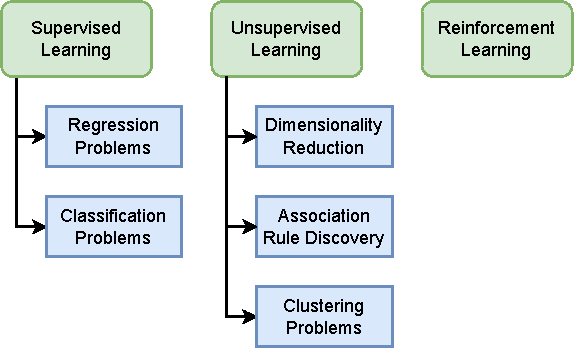
\includegraphics[width=0.7\textwidth]{figs/ml_types.pdf}
    \caption[Overview of \ac{ml} Learning Paradigms]{Comprehensive taxonomy of \ac{ml}, detailing its three fundamental learning paradigms: Supervised Learning, Unsupervised Learning, and Reinforcement Learning, and their associated problem domains.}
    \label{fig:ml_types}
\end{figure}

Supervised learning is used when the data is labeled, and the goal is to predict the output based on the input data. This type of learning is used in classification problems, where the output is a category, and regression problems, where the output is a continuous value. 

Unsupervised learning is used when the data is not labeled and the goal is to find patterns in it. This is used in clustering problems, where the goal is to group similar data points together, association rule discovery problems, where the goal is to find relationships between variables, and dimensionality reduction problems, where the goal is to reduce the number of variables in the data.

Finally, reinforcement learning is used when the agent learns to interact with the environment by taking actions and receiving rewards. The goal is to learn a policy that maximizes the cumulative reward.

Given that the data is centralized, the training process can be done on a single machine, without the need for communication between different entities. This makes the training process easier to implement, monitor, and resource-efficient. However, it also has some drawbacks, such as privacy concerns when the data is sensitive or confidential, a single point of failure, and scalability issues when the data or the model is too large to be computed by a single machine.

\subsection{Neural Networks}
\label{sec:neural-networks}

\ac{nn} represent a fundamental and powerful class of models in \ac{ml}, particularly central to the field of deep learning. While centralized \ac{ml} can employ various model types, \acp{nn} are frequently used due to their ability to learn complex patterns.

A \ac{nn} is structured in layers, typically including an input layer, one or more hidden layers, and an output layer. Each layer consists of interconnected nodes (or neurons), with connections having associated weights and biases. During training, data passes through the \ac{nn} (forward pass), and calculations are performed at each neuron using activation functions, resulting in a prediction. The difference between the prediction and the actual target is quantified by a loss function. 

To minimize this loss, the \ac{nn} is trained using algorithms like backpropagation \cite{rumelhart1986learning}, which calculates the gradients of the loss function concerning the \ac{nn}'s weights and biases. These gradients indicate the direction and magnitude of the change needed for each weight and bias to reduce the loss. Various optimization methods (e.g., Gradient Descent, Adam \cite{kingma2014adam}) then use these gradients to update the weights and biases, iteratively improving the model's performance. 

A simple representation of an \ac{nn} structure is shown in Figure \ref{fig:nn_structure}. The input layer receives the data, the hidden layers process it, and the output layer produces the final prediction. Each connection between neurons has a weight that determines its influence on the output.

\begin{figure}[!htb]
    \centering
    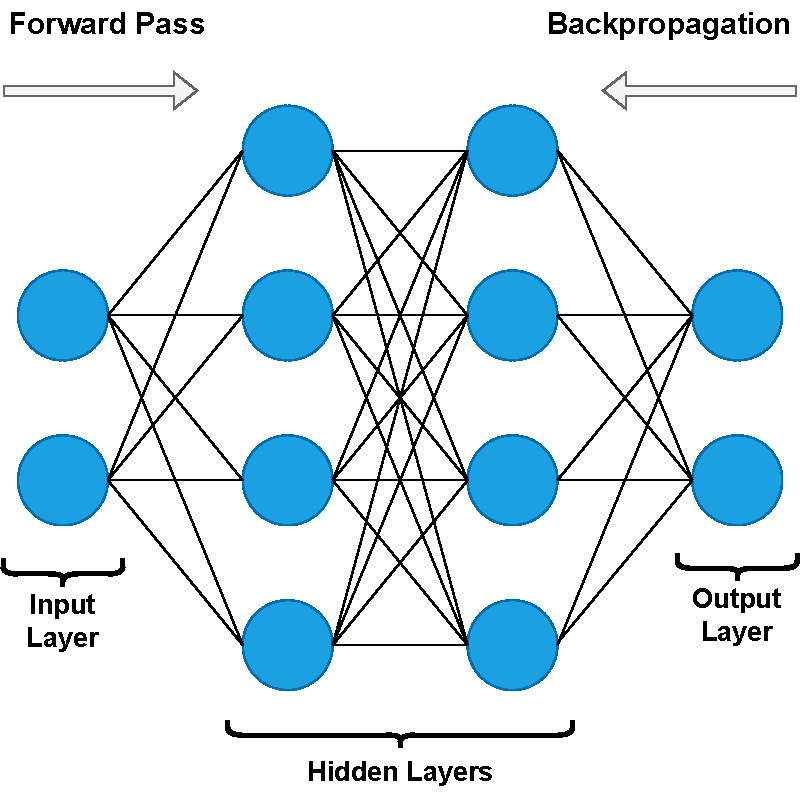
\includegraphics[width=0.6\textwidth]{figs/nn_structure.pdf}
    \caption[Neural Network Structure]{Structure of a typical Neural Network, detailing its Input, Hidden, and Output Layers. The diagram highlights the directional flow of computation during the Forward Pass and the gradient-based optimization process of Backpropagation.}
    \label{fig:nn_structure}
\end{figure}

In the context of distributed and \ac{fl}, the model being trained is often a \ac{nn}. It is crucial to distinguish this model network structure from the communication network of interconnected devices (workers and servers) participating in the distributed learning process. For the remainder of this dissertation, we use the term Model to refer specifically to a \ac{nn}, and Network to denote a communication network, unless otherwise stated.



\section{Distributed Machine Learning}
\label{sec:distributed-ml}

Distributed \ac{ml} is an approach where the data or model is distributed across multiple machines and the training process is done in a distributed manner that, under certain conditions, enables faster training and allows larger models and datasets that can't be processed by a single machine \cite{10410765, 10608461}. 

The distributed training process can follow different architectures and techniques. In \cite{9120226}, the authors present a taxonomy that classifies distributed \ac{ml} into three categories: Model vs Data Parallelism, Centralized vs Decentralized Optimization, and Synchronous vs Asynchronous Scheduling.

\subsection{Model vs Data Parallelism}
\label{sec:model-vs-data-parallelism}

Model and Data Parallelism are two different strategies for distributing large workloads, one maps the model to multiple machines, and the other maps the data to multiple machines.

Model parallelism involves dividing a \ac{ml} model into partitions to be processed by different machines, and it is particularly beneficial when the model is too large to fit in memory. This partitioning can be done in two ways: vertical partitioning, which splits the model between layers, or horizontal partitioning, which divides individual layers as shown in Figure \ref{fig:model_parallelism}.

\begin{figure}[!htb]
    \centering
    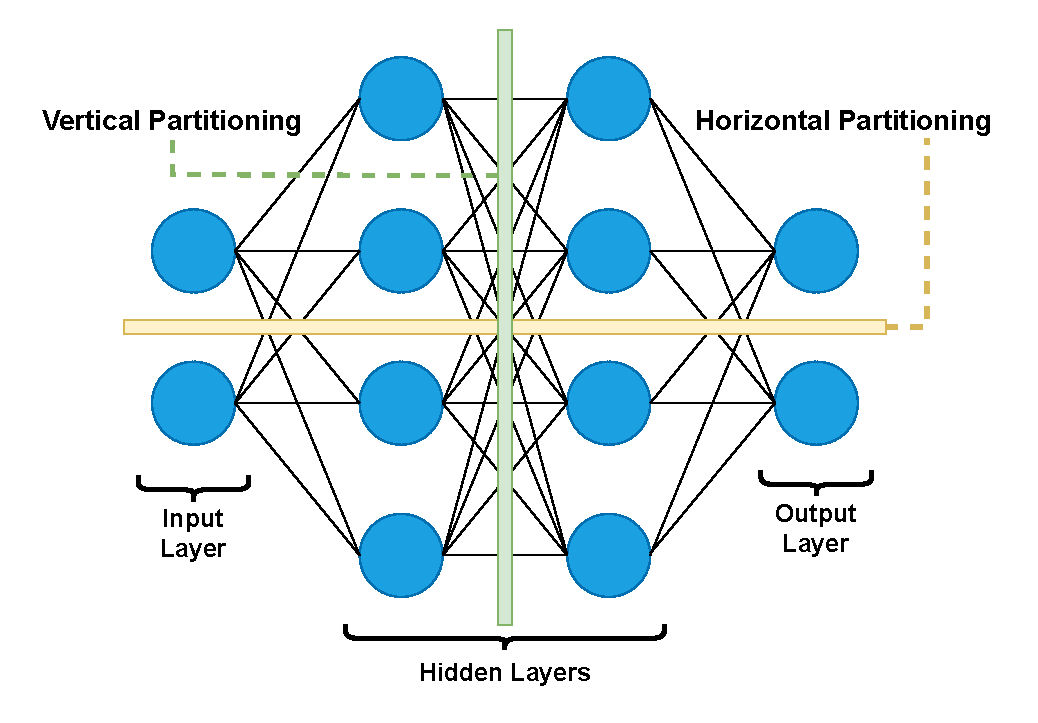
\includegraphics[width=0.7\textwidth]{figs/model_parallelism.pdf}
    \caption[Model Parallelism Partitioning]{Illustration of Model Parallelism, distinguishing between Vertical Partitioning, where the model is split across layers, and Horizontal Partitioning, where individual layers are divided across multiple machines.}
    \label{fig:model_parallelism}
\end{figure}

Vertical partitioning is simpler to implement since it requires transporting intermediate outputs (activations) between machines. On the other hand, horizontal partitioning, which splits the layers themselves, is more complex because it requires managing numerous inter-machine connections.

In data parallelism, multiple machines process different subsets of the data using the same model architecture. This approach aggregates gradients or weights from various machines to update the model parameters, facilitating parallelized computation. The communication overhead and scalability depend on the model size and the efficiency of the aggregation mechanism. Data parallelism is often easier to implement and scale than model parallelism, allows data privacy when combined with privacy-preserving techniques, and is widely adopted in distributed systems.

\subsection{Centralized vs Decentralized Optimization}
\label{sec:centralized-vs-decentralized-optimization}

In centralized optimization, a central server (parameter server) aggregates gradients computed by distributed workers and updates the global model parameters. While this architecture simplifies the synchronization and coordination of workers, it can become a bottleneck in large clusters due to communication overhead and reliance on a single server for updates, because the gradients are sent to the parameter server after each batch, and the updated weights are sent back to the workers. Advanced implementations mitigate these issues by distributing the parameter server role across multiple nodes. Figure \ref{fig:centralized_opt} shows the centralized optimization process.

\begin{figure}[!htb]
    \centering
    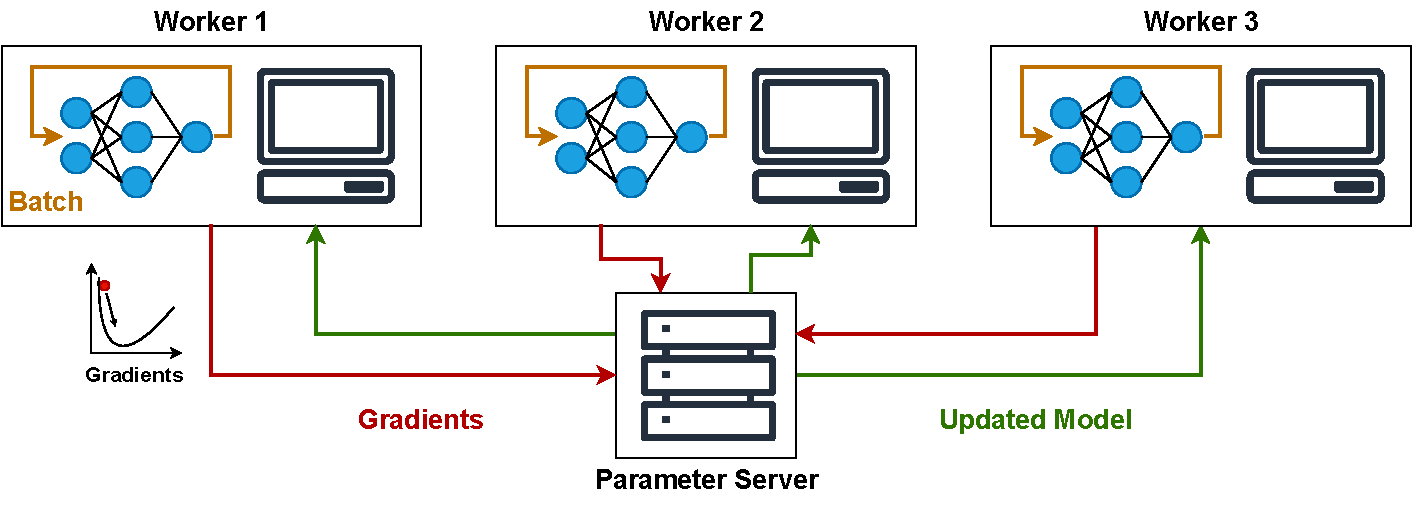
\includegraphics[width=\textwidth]{figs/centralized_opt.pdf}
    \caption[Centralized Optimization Process]{Diagram illustrating the Centralized Optimization process, where multiple Workers compute gradients and send them to a single Parameter Server, which then aggregates these gradients to update the global model and sends the Updated Model back to the workers.}
    \label{fig:centralized_opt}
\end{figure}

Decentralized optimization involves each worker training its local model independently, periodically synchronizing with peers or a master node (parameter server) by sending the weights. This method can reduce dependency on a central server, enabling higher scalability and tolerance to communication delays. However, ensuring convergence and minimizing inconsistencies among workers requires careful tuning of synchronization strategies and hyperparameters. Figure \ref{fig:decentralized_opt} shows the decentralized optimization process.

\begin{figure}[!htb]
    \centering
    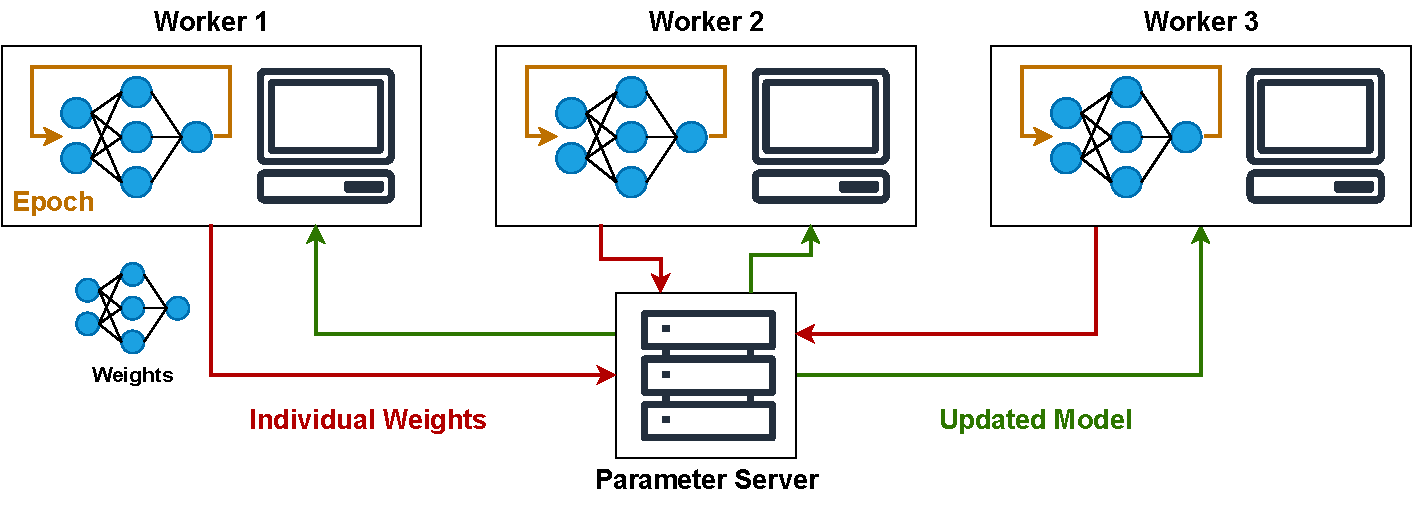
\includegraphics[width=\textwidth]{figs/decentralized_opt.pdf}
    \caption[Decentralized Optimization Process]{Diagram illustrating the decentralized optimization process, where workers train their local models independently and periodically synchronize with a parameter server by exchanging individual weights and receiving updated models.}
    \label{fig:decentralized_opt}
\end{figure}

These two approaches can then be used together or individually in a hierarchical manner \cite{liu2020client}, where the workers are divided into groups, each group has a master node, and the parameter server aggregates the gradients or weights from the master nodes. This approach can reduce the communication overhead and improve the system's scalability.

\subsection{Synchronous vs Asynchronous Scheduling}
\label{sec:synchronous-vs-asynchronous-scheduling}

In synchronous systems, workers operate in lockstep, aggregating all updates before proceeding to the next training iteration. This approach minimizes inconsistencies among workers and is easier to implement and debug, but it can lead to resource underutilization due to waiting for slower nodes (stragglers). Model aggregation in synchronous systems typically uses weighted averaging, where each worker's update is scaled based on factors such as data size or importance before being combined into a global model.

The weighted averaging is defined as follows:
\begin{equation}
    \theta_{t+1} = \frac{\sum_{i=1}^{N} w_i \cdot \theta_i}{\sum_{i=1}^{N} w_i}
\end{equation}

where $\theta_{t+1}$ is the updated model parameters, $N$ is the number of workers, $w_i$ is the weight assigned to worker $i$, and $\theta_i$ is the model parameters from worker $i$. The weights are typically proportional to each worker’s data size or reliability. The normalization ensures that the update is a true weighted average, maintaining scale consistency and promoting a balanced aggregation.


Asynchronous systems allow workers to proceed with their computations independently, updating the model parameters as they complete their tasks. While this maximizes resource utilization and can be more scalable, it introduces challenges such as stale updates, which can slow convergence or degrade model performance. To mitigate this, linear interpolation is often used for model aggregation, blending new updates with the current model state to maintain stability. These complexities make asynchronous systems harder to implement and debug, but potentially more efficient in heterogeneous environments.

The linear interpolation is defined as follows:
\begin{equation}
    \theta_{t+1} = \theta_t + \alpha \cdot (\theta_i - \theta_t)
\end{equation}

where $\theta_{t+1}$ is the updated model parameters, $\theta_t$ is the current model parameters, $\alpha$ is the interpolation factor (0 < $\alpha$ < 1), and $\theta_i$ is the model parameters from worker $i$. This allows the system to blend new updates with the current model state, maintaining stability while incorporating fresh information.



\section{Federated Learning}
\label{sec:federated-learning}

\ac{fl} is a paradigm of distributed \ac{ml},  which can differ from other distributed \ac{ml} approaches in three ways \cite{liu2022distributed}. First, the data cannot be shared between the devices, ensuring privacy, security, and ownership. This way, laws and regulations such as the \ac{gdpr} are easier to comply with. Second, \ac{fl} is designed to work in a distributed manner, while maximizing resource utilization, allowing organizations to collaborate without sharing data. Finally, \ac{fl} can have security mechanisms such as encryption to further protect the data.

The core process of \ac{fl}, where training is coordinated across multiple devices while keeping data local, is illustrated in Figure \ref{fig:fl_process}. 

\begin{figure}[!htb]
    \centering
    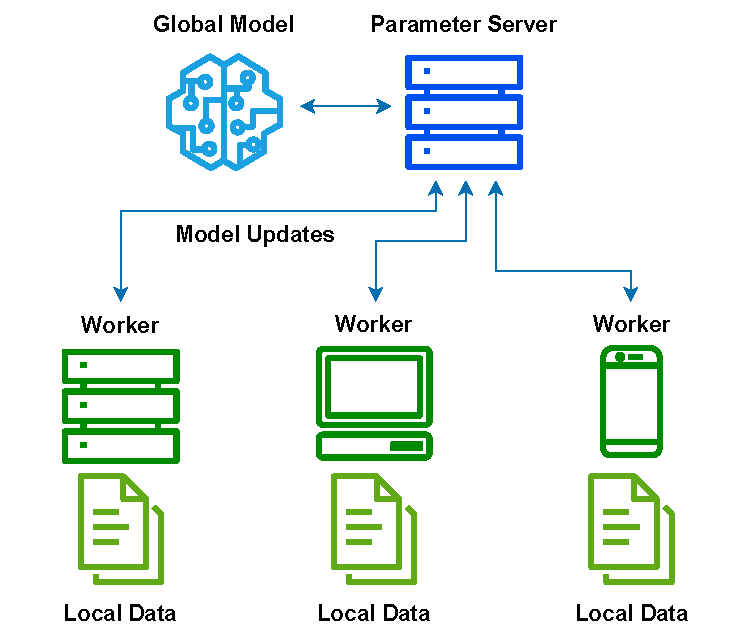
\includegraphics[width=0.7\textwidth]{figs/fl_process.pdf}
    \caption[Federated Learning Process Overview]{The core process of Federated Learning, illustrating how a central Parameter Server coordinates model training across multiple Workers, where each Data remains stored locally, ensuring privacy and security by only exchanging Model Updates for a Global Model.}
    \label{fig:fl_process}
\end{figure}

\ac{fl} can be divided into three main categories: horizontal \ac{fl}, vertical \ac{fl} and federated transfer learning \cite{yang2019federated}. Horizontal \ac{fl} is applicable when the datasets of participating entities share the same feature space but have different samples \cite{yang2020horizontal}. Vertical \ac{fl} is used when the datasets share the same samples but have different features \cite{liu2024vertical}. Federated transfer learning is used when the datasets have different feature spaces and samples, and the goal is to transfer knowledge from one dataset to another \cite{saha2021federated}.

Most of the \ac{fl} use cases are related to mobile devices, industrial engineering, and healthcare, where the data is sensitive and cannot be shared, or the centralized approach is not feasible due to the large amount of data \cite{li2020review}. When these restrictions do not apply, the other approaches might be more suitable.

\section{Communication Protocols}
\label{sec:communication-protocols}

\ac{fl} relies on efficient communication protocols to manage distributed training, ensuring privacy, scalability, and minimal overhead. The protocol choice depends on the system requirements, such as the number of devices, network conditions, and security constraints. This section evaluates the scalability, fault tolerance, security, and suitability for \ac{fl} applications of four prominent communication protocols: \ac{mpi} \cite{gabriel2004open}, \ac{mqtt} \cite{light2017mosquitto}, Kafka \cite{kreps2011kafka}, and Zenoh \cite{corsaro2023zenoh}, while highlighting their key features and limitations.

\subsection{MPI}
\label{sec:mpi}

\ac{mpi} is a widely used communication protocol in \ac{hpc} environments, providing low-latency, high-throughput communication between nodes, because it is designed to handle the message-passing paradigm with explicit exchange of data by send and receive operations. 

However, \ac{mpi} relies on static configurations, requiring predefined communication endpoints and also lacks built-in support for fault tolerance, making it unsuitable for handling worker disconnections or failures, which are common in real-world \ac{fl} systems. 

While its synchronous communication model ensures consistency, it introduces constraints that hinder scalability in flexible, decentralized training scenarios. Additionally, \ac{mpi} does not provide native support for encryption or authentication, relying instead on secure underlying transport layers like \ac{ssh} or network-level security configurations.

Figure \ref{fig:mpi_comm} illustrates the basic communication flow in an \ac{mpi} system, where processes exchange messages explicitly.

\begin{figure}[!htb]
    \centering
    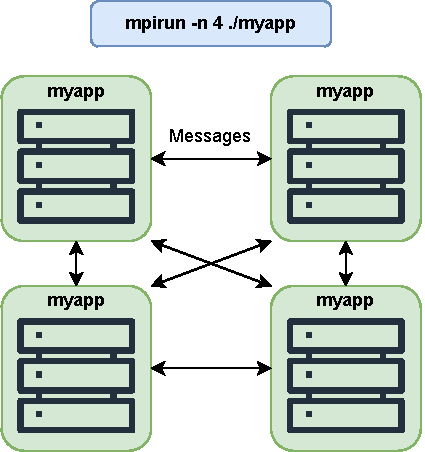
\includegraphics[width=0.45\textwidth]{figs/mpi_comm.pdf}
    \caption[MPI Communication Flow]{The communication flow within an \ac{mpi} system, showing four interconnected application processes. This setup relies on a static configuration, where the number of workers is fixed and new participants cannot dynamically join, with all processes typically executing the same program.}
    \label{fig:mpi_comm}
\end{figure}

\subsection{MQTT}
\label{sec:mqtt}

\ac{mqtt} is a lightweight publish-subscribe protocol designed for resource-constrained devices and low-bandwidth networks. It employs a centralized broker to mediate client communication, allowing devices to dynamically join or leave the system without disrupting operations, making it appealing for \ac{fl} use cases. 

It also offers a native way to notify clients when other clients disconnect, which is helpful for \ac{fl} systems where worker availability may fluctuate. Despite its advantages for edge deployments, this centralized architecture can become a bottleneck in large-scale deployments, particularly as the volume of exchanged model updates increases. 

\ac{mqtt} supports \ac{tls} and \ac{mtls} for secure communication on top of \ac{tcp}, with client authentication and role-based access control. However, the dependence on a broker limits scalability compared to fully decentralized protocols.

Figure \ref{fig:mqtt_comm} illustrates the communication flow in an \ac{mqtt} system, where clients publish messages to topics and subscribe to receive updates.

\begin{figure}[!htb]
    \centering
    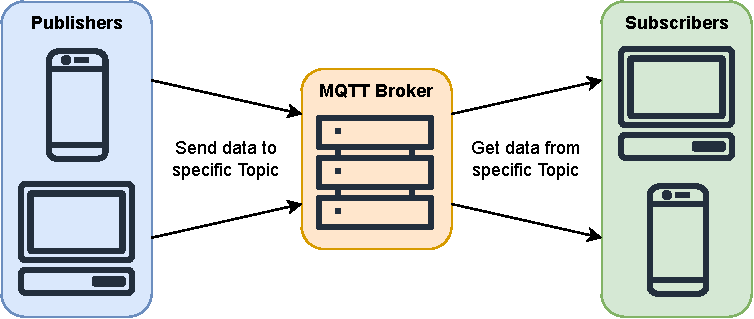
\includegraphics[width=0.75\textwidth]{figs/mqtt_comm.pdf}
    \caption[MQTT Communication Flow]{Illustration of the \ac{mqtt} communication flow, showcasing the publish-subscribe model. Publishers send data to a central \ac{mqtt} Broker, which then mediates the distribution of messages to relevant Subscribers based on specific topics.}
    \label{fig:mqtt_comm}
\end{figure}

\subsection{Kafka}
\label{sec:kafka}

Kafka is a distributed streaming platform optimized for real-time data processing. Its publish-subscribe model supports dynamic and large-scale systems, offering persistent storage and robust fault tolerance through distributed broker clusters. 

However, Kafka's suitability for \ac{fl} is hindered by the latency introduced through its brokered communication model, where the additional communication hops required for routing messages through brokers can slow down the synchronization of model updates, which is critical in iterative training processes. 

The only native disconnection notification mechanism is inspection of connected groups. To participate in a group, clients must subscribe with the same group ID, but this approach adds considerable overhead because when a client joins or leaves, partitions must be rebalanced, which can be time-consuming and resource-intensive.

Similarly to \ac{mqtt}, Kafka supports \ac{tls}, \ac{mtls}, client authentication, and role-based access control for secure communication.

Figure \ref{fig:kafka_comm} illustrates the communication flow in a Kafka system, where producers publish messages to topics and consumers subscribe to receive updates.

\begin{figure}[!htb]
    \centering
    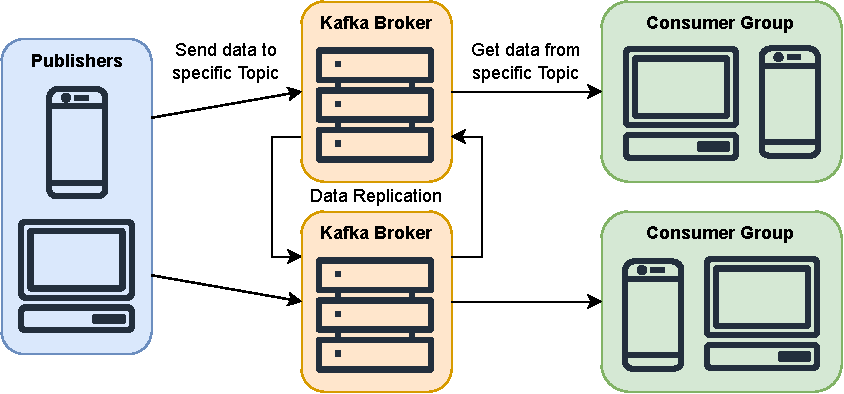
\includegraphics[width=0.9\textwidth]{figs/kafka_comm.pdf}
    \caption[Kafka Communication Flow]{Illustration of the Kafka communication flow, detailing how Publishers send data to topics managed by a distributed Kafka Broker cluster. This system leverages data replication for persistence and fault tolerance, and messages are consumed by organized Consumer Groups from specific topics.}
    \label{fig:kafka_comm}
\end{figure}

\subsection{Zenoh}
\label{sec:zenoh}

Zenoh is a decentralized communication middleware specifically designed for dynamic and resource-constrained environments. Unlike broker-based protocols, Zenoh adopts a fully decentralized architecture that eliminates single points of failure and enables seamless communication among devices, even in unreliable network conditions. 

Similar to \ac{mqtt}, it offers a native way that allows participants to be notified when other participants leave the network without needing a centralized broker.

It supports multiple communication methods, including \ac{tcp}, \ac{tls} and \ac{mtls}, allowing devices to adapt to varying security and performance requirements. Zenoh also supports the use of \acp{acl}, enabling fine-grained permission management to control which entities can publish or subscribe to specific data. Despite its advantages, Zenoh is a relatively new protocol with a less mature ecosystem compared to established solutions such as the ones mentioned above, which may limit its adoption in existing \ac{fl} systems.

Figure \ref{fig:zenoh_comm} illustrates the communication flow in a Zenoh system, where devices communicate directly without a central broker and can join or leave the network dynamically.

\begin{figure}[!htb]
    \centering
    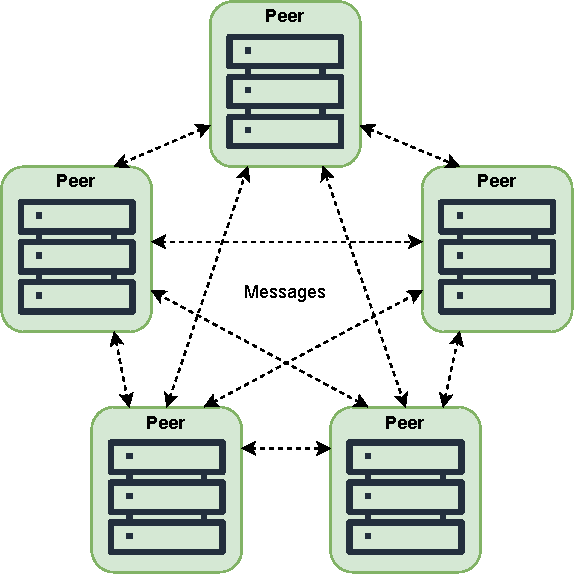
\includegraphics[width=0.6\textwidth]{figs/zenoh_comm.pdf}
    \caption[Zenoh Communication Flow]{Illustration of the Zenoh communication flow, highlighting its fully decentralized peer-to-peer architecture. This design allows individual Peers to communicate directly and dynamically join or leave the network at any moment without requiring a central broker. Adapted from Zenoh Documentation.}
    \label{fig:zenoh_comm}
\end{figure}


\subsection{Summary of Communication Protocols}

Communication protocols are critical to enable efficient, secure, and scalable \ac{fl} systems. Each protocol discussed offers unique strengths and limitations, making them suitable for different scenarios. The choice of protocol should be based on the specific requirements of the \ac{fl} system, such as the number of devices, network conditions, and security constraints, to ensure optimal performance and reliability.

Table~\ref{tab:communication_protocols} summarizes the communication protocols' main features, highlighting their suitability for our scenario.

\begin{table}[!htb]
    \caption[Comparative Analysis of FL Communication Protocols]{A comparative analysis of communication protocols, including \ac{mpi}, \ac{mqtt}, Kafka, and Zenoh, detailing their characteristics in terms of scalability, fault tolerance, security, and general suitability for \ac{fl} deployments.}
    \label{tab:communication_protocols}
    \centering
    \begin{tabular}{Sc Sc Sc Sc Sc}
    \toprule
    \textbf{Protocol} & \textbf{Scalability} & \textbf{Fault Tolerance} & \textbf{Security} & \textbf{Suitability} \\
    \midrule
    \ac{mpi}  & 
        Limited &
        \begin{tabular}[c]{@{}c@{}}No built-in\\support\end{tabular} & 
        Relies on \ac{ssh} & 
        \begin{tabular}[c]{@{}c@{}}Low, lacks fault\\tolerance and scalability\end{tabular} \\
    \ac{mqtt} & 
        Moderate &
        Moderate &
        \begin{tabular}[c]{@{}c@{}}\ac{tls}, \ac{mtls}\\role-based\end{tabular} &
        \begin{tabular}[c]{@{}c@{}}High, suitable when\\using a central broker\end{tabular} \\
    Kafka & 
        High &
        High &
        \begin{tabular}[c]{@{}c@{}}\ac{tls}, \ac{mtls}\\role-based\end{tabular} &
        \begin{tabular}[c]{@{}c@{}}Moderate, latency can\\hinder synchronization\end{tabular} \\
    Zenoh & 
        High &
        High &
        \begin{tabular}[c]{@{}c@{}}\ac{tls}, \ac{mtls}\\\ac{acl}\end{tabular} &
        \begin{tabular}[c]{@{}c@{}}High, but limited\\ecosystem maturity\end{tabular} \\
    \bottomrule
\end{tabular}
\end{table}

In our case, a centralized server (parameter server) coordinates the training process, and the system is designed to be resilient to worker disconnections. This means that a centralized communication broker such as \ac{mqtt} is not a problem, and the system can benefit from its lightweight nature. However, \ac{mpi} is unsuitable for our system because it is designed for static configurations.



\section{Systematic Literature Review}
\label{sec:slr}

The state-of-the-art in \ac{fl} is vast and diverse; however, studies focusing on the type of resilience for this work are harder to find. To address this challenge, a systematic literature review was conducted.

The first step in the review process was to define the research questions that will guide the search for relevant literature. The following questions were defined:

\begin{itemize}
    \item \textbf{RQ1:} How can Federated Learning frameworks be designed to ensure robustness against node failures across dynamic network environments?
    \item \textbf{RQ2:} What communication layer architectures are most suitable for supporting fault-tolerant and resilient Federated Learning under dynamic network conditions?
\end{itemize}

The first research question aims to understand the strategies and mechanisms that can be used to improve the robustness of \ac{fl} frameworks, while the second question focuses on the communication layer, which is a critical component for the success of \ac{fl} in dynamic networks. These questions aim to identify keywords and concepts that can be used to search for relevant literature.

The next step was to define the queries that would be used to search for relevant literature in databases, specifically SCOPUS. To narrow the search and improve the quality of the results, only records from journals and conferences published in the last five years were considered.

Keywords such as ''Federated Learning'', ''Resilience'', ''Communication'' and ''Fault Tolerance'' emerge from the research questions, but some challenges remain to be addressed. 

For instance, the term ''Resilience'' in \ac{fl} is primarily used in the context of attacks, data poisoning, and to ensure that the \ac{ml} models converge. With the term ''Communication'', most of the results are related to papers focusing on communication costs, communication efficiency, or just an analysis of the communication layer, not including fault tolerance to node failures or network delays. 

Therefore, the query with the most relevant results was: TITLE-ABS-KEY ( ''federated learning'' ) AND TITLE-ABS-KEY ( ''fault tole*'' ).

The review process, as shown in Figure~\ref{fig:prisma}, started with retrieving 121 records from SCOPUS using the previously defined query and filters. This step was conducted on October 31, 2024.

\begin{figure}[!htb]
    \centering
    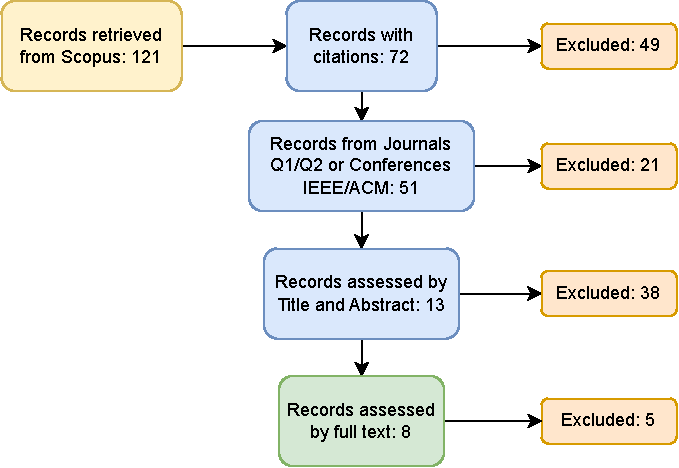
\includegraphics[width=0.8\textwidth]{figs/prisma.pdf}
    \caption[Systematic Literature Review Process]{Detailed flow of the systematic literature review process, beginning with 121 retrieved records from SCOPUS. The diagram illustrates five sequential exclusion steps that systematically filtered irrelevant studies, culminating in a final set of 8 relevant records for in-depth analysis.}
    \label{fig:prisma}
\end{figure}

Studies without citations were excluded from these records to focus on work that has had an observable impact on the research community. This step reduced the pool to 72 records, excluding 49 records.

Given the proven quality and reputation of Journals Q1 and Q2 and Conferences IEEE and ACM, only records from these sources were considered, where 51 records were selected and 21 were excluded.

The next step was to screen the records by title and abstract, to identify studies relevant to the research questions, namely those that focus on fault tolerance of node failures and communication layer architectures. This step reduced the pool to 13 records, while 38 records were excluded. The main reasons for exclusion were: implementation in blockchain, focus on data privacy, and studies that the content overlaps with the problems mentioned before, with the ''Resilient'' and ''Communication'' queries.

While blockchain is a valid approach to ensure fault tolerance and data privacy, the implementation requires a different set of tools and knowledge, adding complexity and overhead to the solution, which is not the focus of this work. 

Finally, a full-text screening was conducted on the remaining 13 records to evaluate their contributions in depth. From these, 5 records were excluded because their focus was security and data encryption, did not specify the communication layer, or how they handle node failures. This resulted in a total of 8 records that were selected for the review.

Each paper has its own contributions and insights, so it is important to analyze and understand each one of them.

In \cite{Bano2021410}, ~\citeauthor{Bano2021410} propose a methodology and architecture to integrate \ac{fl} with Apache Kafka. Although the authors did not implement the solution, they highlight the potential of using Kafka to improve  scalability while ensuring fault tolerance. They also note that integrating this pub/sub system with \ac{fl} is not trivial.

The authors of \cite{Awan2023120918} introduce a novel communication protocol, SEPP-IoT, designed for secure, efficient, and fault-tolerant communication in \ac{fl} systems. Their \ac{fl} framework has five key components: \ac{iot} devices, Central Server, Communication Protocol, Model Management, and Trust Management. With this architecture, the system uses lightweight cryptography, data compression, a reputation-based trust model to identify malicious nodes, and a novel model aggregation mechanism. To ensure fault tolerance, the authors have error detection and correction that involves redundancy checks, and to handle node failures, tasks are reassigned to other nodes. This framework is evaluated with 100 \ac{iot} devices with the MNIST dataset and compared with two existing techniques, \cite{stergiou2023security} and \cite{venu2022secure}. The results show that this framework outperforms the existing methods regarding accuracy, time, memory, and communication overhead.

In \cite{Jayaram2022180}, ~\citeauthor{Jayaram2022180} present a new adaptive and scalable architecture for \ac{fl} aggregation, called AdaFed. This design leverages serverless/cloud functions to aggregate the models, using a logical tree topology for hierarchical aggregation. This way, the system reduces communication overhead and scales up or down based on the number of devices, allowing tolerance to node failures. The authors evaluate the performance of AdaFed in a kubernetes cluster and compare to methods that use static tree-based aggregation, achieving up to 85\% reduction in resources and cost savings.

The authors of \cite{Song20233047}, propose EPPDA, a privacy-preserving data aggregation scheme for \ac{fl}. This work focuses on improving privacy and security by resisting reverse attacks, while maintaining low communication overhead and fault tolerance. The authors use homomorphic secret sharing and encryption, ensuring the server cannot reconstruct individual updates. When a user disconnects, the server can still aggregate the updates from the remaining users. Compared to \cite{bonawitz2017practical}, the proposed scheme offers lower computation cost, reduces error rate, and improves communication efficiency, but its evaluation is only a theoretical analysis.

In \cite{Mansouri2022146} the authors design a threshold-variant of the Joye-Libert secure aggregation scheme. Their secure and fault-tolerant \ac{fl} framework uses this technique to protect clients' updates and aggregate them, while tolerating up to 1/3 of node failures. They compare their protocol with SecAgg and achieve up to 8x faster running times when using 1000 clients.

The authors of \cite{Chen20241} introduce MCHFL, a \ac{fl} framework that uses a distributed network of global aggregation centers located at the edge, replacing the traditional single central server architecture and improving fault tolerance. They compare MCHFL with three existing works, \cite{konevcny2016federated}, \cite{sattler2020clustered} and \cite{liu2020client} with three datasets: MNIST, FashionMNIST and CIFAR-10. Their results show that MCHFL outperforms the existing works in terms of robustness to failures, accuracy, time, and communication costs.

In \cite{Morell202253}, the authors propose a novel algorithm for federated edge learning that adapts to asynchronous clients joining and leaving the computation. Their key features include dynamic self-adaptation to collaboration device variations, interoperability between web browsers and Python processes, and recovering from unexpected disconnections. To achieve this, the authors based their architecture on six actors: the initiator, the workers, the aggregator, the logical server, the distributed in-memory database, and the queue server. This algorithm is evaluated with the MNIST dataset and by leveraging a combination of adaptive aggregation strategies and efficient communication between its architectural components, the algorithm achieves high levels of accuracy and \ac{ck} score, even in highly volatile environments and \ac{non-iid} data distributions. 

In \cite{Dautov2024110}, ~\citeauthor{Dautov2024110} propose a novel approach to improve fault tolerance and self-recovery in \ac{fl} systems by integrating the Raft consensus protocol. Their method allows nodes in an \ac{fl} cluster to replicate the global state and dynamically elect a new aggregator upon failures, addressing the single-point-of-failure issue. The authors implement their approach as a proof of concept using the Flower \ac{fl} framework, enhanced with PySyncObj, and test it on a Raspberry Pi cluster. Their evaluation on the CIFAR-10 dataset shows that the system achieves aggregator re-election within 4 seconds for clusters of up to 10 nodes and ensures training continuity from checkpoints. However, the Raft-based implementation has a network traffic overhead approximately five times higher than baseline systems due to state replication and leader election.

To better understand the contributions of these papers, we can categorize them into common topics found in the literature. These topics help to identify strengths and limitations, as well as to understand the gaps in the research field. The topics are:

\begin{itemize}
    \item \textbf{Fault Tolerance:} Whether the solution can handle node failures and keep the system running or not.
    \item \textbf{Elasticity:} Ability to handle dynamic networks, where devices can join or leave the network at any time.
    \item \textbf{Scalability:} Number of workers used in the evaluation, to understand if the solution can handle a large number of devices.
    \item \textbf{Security:} Use of encryption or other security mechanisms to protect communication.
    \item \textbf{Evaluation:} Use of standard datasets and benchmarks to evaluate the performance of the solution.
    \item \textbf{Code Availability:} If the code is available for the community to use and reproduce the results.
\end{itemize}

The Compliance column represents the overall alignment of each related work with the desired characteristics for a robust and scalable \ac{fl} framework, particularly those relevant to dynamic and resource-constrained edge environments. This percentage reflects how comprehensively each study addresses the various dimensions presented in the table, with each dimension considered to have equal importance/weight in the context of our proposed system's objectives.

\begin{table}[!htb]
    \caption[Categorization of Reviewed Papers]{Categorization of the 8 selected papers from the systematic literature review, classifying each study based on its demonstrated capabilities and contributions across key topics such as fault tolerance, elasticity, scalability, security, evaluation methods, and code availability}
    \label{tab:topics_summary}
    \centering
    \resizebox{\textwidth}{!}{%
    \begin{tabular}{Sc Sc Sc Sc Sc Sc Sc Sc}
    \toprule
    \textbf{Ref} & 
    \textbf{\begin{tabular}[c]{@{}c@{}}Fault\\ Tolerance\end{tabular}} &
    \textbf{Elasticity} & \textbf{Scalability} & \textbf{Security} & \textbf{Evaluation} & \textbf{Code} & \textbf{Compliance} \\
    \midrule
    \cite{Bano2021410}  & \checkmark & X & Not tested & \checkmark & X & X & \gtext{33} \\
    \cite{Awan2023120918} & \checkmark & X & 1000 & \checkmark & \checkmark & X & \gtext{66} \\
    \cite{Jayaram2022180} & \checkmark & \checkmark & 10000 & X & \checkmark & X & \gtext{66} \\
    \cite{Song20233047} & \checkmark & X & 400 & \checkmark & X & X & \gtext{50} \\
    \cite{Mansouri2022146} & \checkmark & X & 1000 & \checkmark & X & \checkmark & \gtext{66} \\
    \cite{Chen20241} & \checkmark & X & 600 & X & \checkmark & X & \gtext{50} \\
    \cite{Morell202253} & \checkmark & \checkmark & 64 & X & \checkmark & \checkmark & \gtext{83} \\
    \cite{Dautov2024110} & \checkmark & X & 10 & X & \checkmark & \checkmark & \gtext{66} \\
    \midrule
    \textbf{Total:} & \gtext{100} & \gtext{25} & \gtext{87.5} & \gtext{50} & \gtext{62.5} & \gtext{37.5} & \\
    \bottomrule
    \end{tabular}%
    }
\end{table}

As shown in Table~\ref{tab:topics_summary}, all the papers have fault tolerance mechanisms, but only 2 out of 8 can handle dynamic networks. Regarding security, the encryption methods include a lightweight stream cipher algorithm, homomorphic encryption, and Shamir's secret sharing. Although the evaluation is done with standard datasets, such as MNIST, CIFAR, and FashionMNIST, these datasets are not representative of real-world scenarios, where \ac{fl} is needed to protect sensitive data; datasets related to \ac{iot} or \acp{ids} are more suitable. Finally, only 3 out of 8 papers have the code available for the community, which is essential to create new solutions or build upon existing ones.


\section{Heterogenous Frameworks}
\label{sec:other-frameworks}

In addition to the papers analyzed in the systematic review, other \ac{fl} frameworks have been developed to address various challenges in \ac{fl}, ranging from scalability and heterogeneity to fault tolerance and dynamic network conditions. These frameworks are: \ac{heterofl}. \ac{cocofl}, Flower, and TensorFlow Federated.

These frameworks provide distinct solutions to the challenges of \ac{fl}, having different strengths and limitations. These are summarized in Table~\ref{tab:frameworks} and are further discussed in Section \ref{sec:system_requirements_and_comparison}.

\begin{table}[!htb]
    \caption[Key Characteristics of Alternative FL Frameworks]{Key characteristics and drawbacks of prominent alternative \ac{fl} frameworks such as \ac{heterofl}, \ac{cocofl}, Flower, and TensorFlow Federated, providing insight into their design philosophies and applicability.}
    \label{tab:frameworks}
    \centering
    \resizebox{\textwidth}{!}{%
    \begin{tabular}{Sc Sc Sc}
    \toprule
    \textbf{Framework} & \textbf{Key Features} & \textbf{Limitations} \\
    \midrule
    HeteroFL & 
    \begin{tabular}[c]{@{}c@{}} Supports heterogeneous client models \\ Static batch normalization \end{tabular} &
    \begin{tabular}[c]{@{}c@{}} Lack of customization \\ Focus on heterogeneity \end{tabular} \\
    CoCoFL &
    \begin{tabular}[c]{@{}c@{}} Partial neural network freezing \\ Quantization \end{tabular} &
    \begin{tabular}[c]{@{}c@{}} Out of the box solution \\ Lack of flexibility \end{tabular} \\
    Flower &
    \begin{tabular}[c]{@{}c@{}} Framework agnostic \\ Customizable and scalable \end{tabular} &
    \begin{tabular}[c]{@{}c@{}} Not a complete solution \\ Requires additional components \end{tabular} \\
    TFF &
    \begin{tabular}[c]{@{}c@{}} Seamless integration with TensorFlow \\ Supports dynamic client participation \end{tabular} &
    \begin{tabular}[c]{@{}c@{}} Restricted to TensorFlow \\ Fixed communication layer \end{tabular} \\
    \bottomrule
    \end{tabular}%
    }
\end{table}


\subsection{HeteroFL}
\label{sec:heterofl}

\ac{heterofl} is a framework presented in \cite{diao2020heterofl} designed to allow clients with heterogeneous resources to participate in \ac{fl} systems. The framework enables clients to use heterogeneous local models with different computational complexities to contribute to the global model, unlike traditional \ac{fl} methods that require all clients to use the same model architecture. 

This is achieved through a novel technique of adaptively distributing subnetworks to clients based on their capabilities, enabling efficient participation without compromising the overall system performance. \ac{heterofl} also introduces key innovations such as static batch normalization to ensure privacy and stability during training, and a scaling mechanism to balance contributions from models of different sizes.

\subsection{CoCoFL}
\label{sec:cocofl}

\ac{cocofl} is a novel framework designed to address the challenges of resource heterogeneity in \ac{fl} systems and presented in \cite{pfeiffer2022cocofl}. Unlike traditional \ac{fl} methods, which can exclude or limit the contributions of devices with constrained resources, \ac{cocofl} ensures fairness and efficiency by introducing partial \ac{nn} freezing and quantization. 

These techniques allow devices to adapt their training process to available computation, communication, and memory resources. \ac{cocofl} can significantly reduce resources by freezing specific \ac{nn} layers and performing low-precision operations on frozen layers. This allows all devices to train on the whole model, ensuring that even less capable devices make meaningful contributions to the global model, preserving accuracy and fairness across participants. 

The framework outperforms existing methods, such as \ac{heterofl}, in environments with \ac{non-iid} data distributions, where weaker devices are critical for capturing diverse data patterns.

\subsection{Flower}
\label{sec:flower}

Flower is a versatile \ac{fl} framework designed for research and deployment across various \ac{ml} frameworks, such as TensorFlow, PyTorch, and JAX. It offers customization, scalability, and framework-agnostic capabilities, making it suitable for diverse \ac{fl} use cases.

Flower emphasizes ease of use, allowing researchers to create and extend \ac{fl} systems, integrate state-of-the-art strategies, and support synchronous and asynchronous approaches. By leveraging Flower's easy-to-use \acp{api}, users can quickly prototype \ac{fl} systems without building everything from scratch, but it is just a tool, not a complete solution.

\subsection{TensorFlow Federated}
\label{sec:tff}

TensorFlow Federated is a framework designed to facilitate \ac{fl} applications within the TensorFlow ecosystem. The framework supports both federated training and evaluation and provides tools for simulating \ac{fl} experiments. It also handles heterogeneous devices and data, which allows dynamic client participation regardless of computational resources. 

This customizable framework enables users to define their \ac{fl} algorithms, models, and data sources. Still, it does not allow users to define their communication layer or use different \ac{ml} frameworks.


\chapter{Proposed Solution}
\label{chap:proposed_solution}

\begin{introduction}

To address the challenges of \ac{fl} in heterogeneous environments, it is essential to identify the core requirements that enable robust and scalable solutions. \ac{fl} frameworks must accommodate dynamic network conditions, varying device capabilities, and constraints such as limited bandwidth and computational power. These requirements are important to develop a system architecture capable of handling these challenges. 

This chapter explores the requirements necessary for designing a resilient \ac{fl} architecture and introduces the proposed system's key components. The analysis begins with an evaluation and comparison of existing frameworks and technologies to establish baseline expectations. The proposed solution is then presented, detailing the system's architecture, components, and design choices. Finally, a SWOT analysis is conducted to assess the system's strengths, weaknesses, opportunities, and threats, providing a comprehensive overview of the proposed solution.

\end{introduction}



\section{System Requirements and Comparison}
\label{sec:system_requirements_and_comparison}

To understand the current state of \ac{fl} solutions, a comparative analysis of existing frameworks shown in Chapter~\ref{chap:background} was conducted. The comparison includes the papers that evaluated their solution, the other frameworks, and is based on the following criteria:

\begin{itemize}
    \item \textbf{Resilience:} The system should be able to maintain the model training even with node failures and allow devices to join or leave the network at any time.
    \item \textbf{Modularity:} The framework should be modular regarding the \ac{ml} backend, \ac{fl} algorithm, and communication layer.
    \item \textbf{Analysis:} The authors should provide a detailed analysis of the proposed solution, explaining their design choices and evaluating the system's performance.
    \item \textbf{Code and Documentation:} Availability of the source code and detailed documentation to help users understand and use the system.
\end{itemize}

These criteria are the minimum requirements for a \ac{fl} framework to handle the challenges of heterogeneous environments and, equally important, to be extended and integrated with other systems. Table~\ref{tab:topics} summarizes the results of the analysis, where each solution, including the proposed solution, is evaluated based on these criteria. 

\begin{table}[!htb]
    \caption[Qualitative Comparison of Proposed and Existing FL Solutions]{A qualitative comparison of the proposed \ac{fl} solution against existing frameworks and research papers, evaluated based on criteria including resilience, modularity, analysis depth, code and documentation availability, and overall compliance with design requirements.}
    \label{tab:topics}
    \centering
    \begin{tabular}{Sc Sc Sc Sc Sc Sc}
    \toprule
    \textbf{Solution} & \textbf{Resilience} & \textbf{Modularity} & \textbf{Analysis} & 
    \textbf{\begin{tabular}[c]{@{}c@{}}Code and \\ Documentation\end{tabular}} & 
    \textbf{Compliance} \\
    \midrule
    \cite{Awan2023120918} & X & X & \checkmark & X & \gtext{25} \\
    \cite{Jayaram2022180} & \checkmark & X & \checkmark & X & \gtext{50} \\
    \cite{Chen20241}      & X & X & \checkmark & X & \gtext{25} \\
    \cite{Morell202253}   & \checkmark & X & \checkmark & \checkmark & \gtext{75} \\
    \cite{Dautov2024110}  & X & X & \checkmark & \checkmark & \gtext{50} \\
    \midrule
    \textbf{HeteroFL}     & \checkmark & X & \checkmark & \checkmark & \gtext{75} \\
    \textbf{CoCoFL}       & \checkmark & X & \checkmark & \checkmark & \gtext{75} \\
    \textbf{Flower}       & X & \checkmark & X & \checkmark & \gtext{50} \\
    \textbf{TTF}          & \checkmark & X & X & \checkmark & \gtext{50} \\
    \midrule
    \textbf{Proposed} & \checkmark & \checkmark & \checkmark & \checkmark & \gtext{100} \\
    \bottomrule
\end{tabular}
\end{table}

While existing solutions and frameworks offer valuable contributions to the field of \ac{fl}, none fully satisfy the specific combination of requirements central to this research: inherent resilience to dynamic network conditions alongside comprehensive modularity across the ML backend, \ac{fl} algorithms, and crucially, the communication layer. 

Frameworks like Flower and TensorFlow Federated provide tools and structures for \ac{fl}, but they either lack the necessary built-in resilience mechanisms to handle arbitrary node failures and dynamic joins/leaves seamlessly without requiring significant additional components. Or they impose restrictions on key modules, particularly the communication protocol, which is vital for adapting to diverse network environments and ensuring fault tolerance. 

The solutions from the systematic review demonstrate analysis and some fault tolerance, but generally lack the modularity and code availability needed for building a highly adaptable open-source platform. 

Therefore, to fully address the identified gaps and achieve the objective of designing, implementing, and evaluating a \ac{fl} framework that is both highly modular and robustly resilient to real-world network dynamics, developing a new framework tailored to these specific goals was deemed necessary.



\section{Architecture}
\label{sec:architecture}

Our proposed framework is not a single, rigid \ac{fl} implementation, but instead a versatile architecture comprising seven core modules that collaborate to support a range of \ac{fl} algorithms and configurations. This modular structure is fundamental to the framework's adaptability, enabling easy integration of new algorithms, communication methods, resilience approaches, and optimizations without requiring substantial modifications to the entire system. Figure~\ref{fig:architecture} shows the architecture of our proposed framework. 

\begin{figure}[!htb]
    \centering
    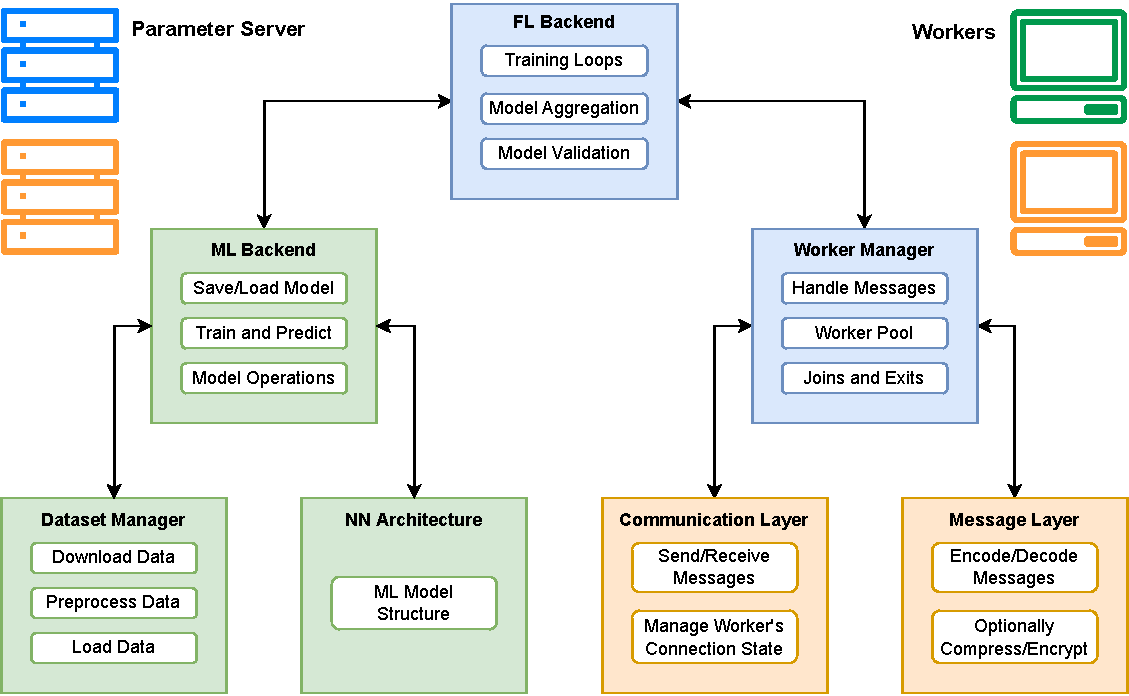
\includegraphics[width=\textwidth]{figs/modules.pdf}
    \caption[Proposed FL Framework Architecture]{Conceptual design of the resilient \ac{fl} system, showcasing its modular components and detailing the roles of the Parameter Server and Workers as key entities. The color-coding helps identify the primary functions of each module within the overall framework.}
    \label{fig:architecture}
\end{figure}

The architecture consists of the following core modules, each serving a specific purpose in the overall system:

\textbf{FL Backend:} This module serves as the central component for the Federated Learning process logic. On the Parameter Server, it manages the global training loop, orchestrates rounds, and determines worker scheduling, aggregates model updates from workers, updates the global model state, and validates it. On the worker side, it manages the local training loop and interaction with the server or peers, depending on the algorithm. It uses the \textit{ML Backend} for model interactions and the \textit{Worker Manager} to interact with workers.

\textbf{ML Backend:} This module provides an abstraction layer for the underlying \ac{ml} framework, making the rest of the framework independent of the specific library used. It handles the \ac{ml} model, offering interfaces for common operations such as saving/loading the model, training the model on local data, making predictions, and other general model operations like accessing weights or gradients. It employs the \textit{Dataset Manager} to retrieve data and the \textit{Neural Network Architecture} to define the model.

\textbf{Dataset Manager:} Responsible for all aspects related to handling data on the client devices. It oversees the data extraction process from local storage, potentially managing tasks like downloading (if data needs to be fetched), preprocessing the data, and loading split data batches for training, validation, and testing. It supplies processed data samples to the \textit{ML Backend}.

\textbf{Neural Network Architecture:} This module defines the structure of the \ac{ml} model being trained. It contains the specifications for the layers and connections of the \ac{nn} and is used by the \textit{ML Backend} to create the model instance before training starts. Separating this allows for straightforward swapping of model architectures for the same dataset or \ac{fl} scenario.

\textbf{Worker Manager:} Primarily located on the Parameter Server, this module manages the pool of participating client devices (workers). It tracks connected workers, handles joins/disconnects from the network, and manages the worker subpool used for each training round (particularly in client-selection scenarios), making it a key component in ensuring the system's elasticity and fault tolerance. It interacts with the workers using the \textit{Communication Layer} and the \textit{Message Layer}, allowing it to encode a message once and send it to multiple workers.

\textbf{Communication Layer:} This vital module handles all network communication between any nodes in the system, including the server and workers. It provides an abstract send and receive interface, concealing the complexities of the specific communication protocol employed. Importantly, this layer is also responsible for providing fundamental resilience to the system by managing connection status, addressing message delivery issues, and incorporating protocol-specific fault tolerance features.

\textbf{Message Layer:} Conceptually positioned below the Communication Layer, this module is responsible for defining the format and processing the content of exchanged messages. It includes functionalities to encode and decode messages and can optionally perform data compression and encryption of model updates or other exchanged information to enhance efficiency and security.

Having detailed the individual roles of the core modules, it is important to explicitly highlight how their collaborative design fulfills the system requirements outlined in Section \ref{sec:system_requirements_and_comparison}. Resilience is a key outcome, achieved through the Worker Manager's dynamic worker pool management and task rescheduling capabilities, ensuring training continuity despite node failures or disconnections. 

The Communication Layer (including the Message Layer for secure and efficient data transfer) further contributes by providing robust fault detection and handling mechanisms. 

Modularity is inherently built into the framework: the ML Backend abstracts diverse machine learning libraries, the FL Backend supports various federated learning algorithms, and the Communication Layer (with its various protocol implementations) allows for flexible integration of communication paradigms. This architectural flexibility, combined with the structured logging by modules like the Worker Manager and FL Backend, facilitates comprehensive Analysis of system performance and training progress. 

The framework's commitment to Code and Documentation is demonstrated by its open-source availability on GitHub and PyPI, alongside its intuitive \ac{cli} tools, making it accessible for researchers and practitioners to understand, use, and extend. Further technical details regarding the implementation of these design choices, including software stack and specific mechanisms, are provided in Chapter \ref{chap:implementation}. 

\section{Communication Strategies}

To further illustrate the proposed architecture's dynamic interactions and resilience mechanisms, particularly in worker participation and task management, we detail the communication sequences during key worker lifecycle events: initial join, network disconnection, and training round participation.

Coordinated by the core modules, these sequences demonstrate the framework's robustness in dynamic environments with fluctuating worker availability.

\subsection{Worker Join Sequence}

When a new worker connects to the system, it undergoes a registration process with the Parameter Server. This handshake establishes its identity and prepares it for participation in the training rounds. This sequence involves the worker initiating contact, the Parameter Server assigning it a unique identifier and a run identifier, and the worker confirming its registration by sending initial metadata before becoming available for tasks. 

The underlying communication protocol primarily handles the initial steps, while the subsequent metadata exchange and readiness signaling involve the Message Layer and Worker Manager. The detailed steps are illustrated in the sequence diagram in Figure~\ref{fig:seq:worker_joins}.

\begin{figure}[!htb]
    \centering
    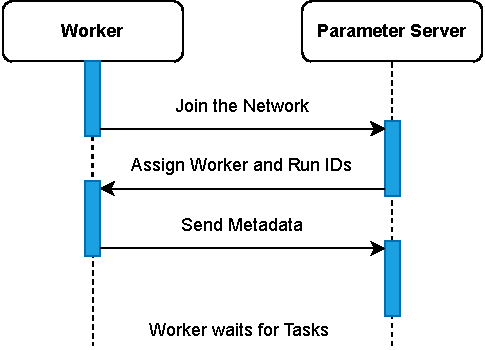
\includegraphics[width=0.5\textwidth]{figs/worker_joins.pdf}
    \caption[Worker Join Sequence in Federated Learning]{Communication sequence illustrating how a worker joins the \ac{fl} system by initiating contact, the Parameter Server assigning unique identifiers, the worker sending initial metadata, and finally, the worker becoming ready to receive tasks.}
    \label{fig:seq:worker_joins}
\end{figure}

\subsection{Worker Leaves Sequence}

Workers may leave the \ac{fl} system either gracefully (sending an explicit disconnect message) or abruptly (due to unexpected disconnections or failures). The framework's resilience relies on the Parameter Server's ability to detect both scenarios and update the active worker pool managed by the Worker Manager accordingly. If a worker sends a leave message, the server receives and processes it. If a worker disconnects unexpectedly, the protocol-specific mechanisms in the Communication Layer detect the loss of connection. Figure~\ref{fig:seq:worker_leaves} illustrates the communication flow for a worker leaving the system.

\begin{figure}[!htb]
    \centering
    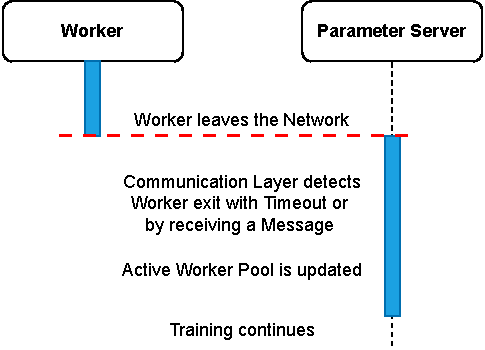
\includegraphics[width=0.5\textwidth]{figs/worker_leaves.pdf}
    \caption[Worker Leaves Sequence in Federated Learning]{Communication sequence illustrating how a worker leaves the \ac{fl} system. The Parameter Server's communication layer detects the worker's exit, either through an explicit message or a timeout, which triggers an update to the active worker pool and allows the training process to continue uninterrupted.}
    \label{fig:seq:worker_leaves}
\end{figure}


\subsection{Work Cycle Sequence}

This sequence depicts the typical communication flow when a worker receives and processes a task during a training round. It starts with the Parameter Server sending the necessary data or model parameters for the task. The worker then performs its local computation (training on its data). Upon completion, the worker returns its results or model updates to the Parameter Server and waits for future messages. The sequence diagram in Figure~\ref{fig:seq:worker_works} illustrates this successful cycle.

\begin{figure}[!htb]
    \centering
    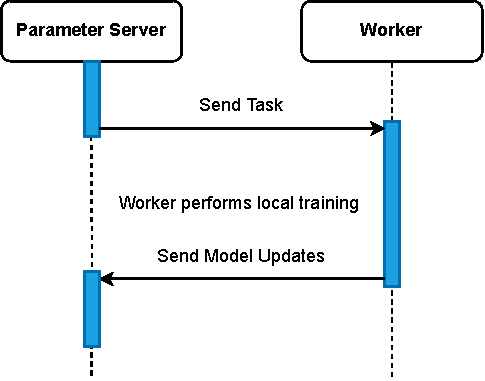
\includegraphics[width=0.5\textwidth]{figs/worker_works.pdf}
    \caption[Worker Task Completion Sequence]{Communication sequence illustrating a worker successfully receiving and completing a task within the \ac{fl} system. The process shows the Parameter Server sending a task, the worker performing local training, and then sending model updates back to the server.}
    \label{fig:seq:worker_works}
\end{figure}

A critical aspect of resilience is handling failures during the work cycle. The Parameter Server must detect if a worker fails after receiving a task but before successfully submitting its results. Depending on the \ac{fl} algorithm (synchronous vs. asynchronous) and the resilience mechanisms implemented (e.g., completion thresholds, task rescheduling by the Worker Manager), the framework adapts to continue training. The sequence diagram in Figure~\ref{fig:seq:worker_fails_work} shows an example of this failure scenario and server detection.

\begin{figure}[!htb]
    \centering
    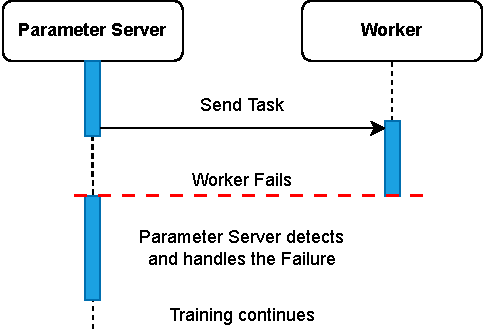
\includegraphics[width=0.5\textwidth]{figs/worker_fails_work.pdf}
    \caption[Worker Failure and Server Detection]{Communication sequence illustrating a worker failure during task execution and the Parameter Server's subsequent detection and handling of this event. This ensures that the \ac{fl} training process can continue despite the disruption.}
    \label{fig:seq:worker_fails_work}
\end{figure}



\section{SWOT Analysis}
\label{sec:swot_analysis}

To provide a comprehensive understanding of the proposed architecture, a SWOT analysis was conducted to evaluate its internal strengths and weaknesses alongside external opportunities and threats. The SWOT analysis is summarized in Table~\ref{tab:swot} and it serves as a guide for future development and evaluation, highlighting areas for improvement and potential risks that must be addressed.

\begin{table}[!htb]
    \caption[SWOT Analysis of the Proposed Solution]{A comprehensive SWOT analysis of the proposed \ac{fl} framework, detailing its internal strengths and weaknesses, alongside external opportunities and threats. This provides a balanced view of its potential and limitations for future development.}
    \label{tab:swot}
    \centering
    \begin{tabular}{Sc | Sc Sc}
    & \textbf{Helpful} & \textbf{Harmful} \\
    \toprule
    \textbf{Internal} & 
    \begin{tabular}[c]{@{}c@{}}\textbf{Strengths} \\
        \addlinespace
        \begin{tabular}[c]{@{}c@{}}Resilient, highly modular \\ and easy to use\end{tabular} \\
    \end{tabular} &
    \begin{tabular}[c]{@{}c@{}}\textbf{Weaknesses} \\ 
        \addlinespace
        \begin{tabular}[c]{@{}c@{}}Validation is limited to \\ the simulation environment\end{tabular} \\
    \end{tabular} \\
    \midrule
    \textbf{External} &
    \begin{tabular}[c]{@{}c@{}}\textbf{Opportunities} \\ 
        \addlinespace
        \begin{tabular}[c]{@{}c@{}}Easy to extend and \\ integrate with other systems\end{tabular} \\
    \end{tabular} &
    \begin{tabular}[c]{@{}c@{}}\textbf{Threats} \\ 
        \addlinespace
        \begin{tabular}[c]{@{}c@{}}Scalability may \\ be limited \end{tabular} \\
    \end{tabular} \\
    \bottomrule
\end{tabular}
\end{table} 


The main strengths are: resilience, modularity, and ease of use. The system is designed to handle dynamic network conditions, ensuring seamless operation even when nodes join or leave the network. The architecture features a highly modular design, working as a puzzle where each piece can be replaced or extended without affecting the other modules. 

Despite its strengths, the system has certain internal weaknesses that may affect its practical utility. The proposed solution will be evaluated in a simulated environment using \acp{vm}. While this provides valuable initial insights, it does not fully replicate real-world conditions. Challenges such as hardware diversity, network instability, and scalability in large-scale deployments are not fully captured in the simulation, limiting the system's validation.

The external opportunities for the proposed solution are vast, as the system is designed to be easily extended and integrated with other systems. This flexibility allows for the integration of new \ac{fl} algorithms, communication protocols, and \ac{ml} models, providing a versatile platform for research and development. The system's modularity also enables the integration of new features and functionalities, allowing for continuous improvement and adaptation to changing requirements.

Finally, the system faces certain external threats that may impact its long-term viability. Despite the system being designed to be scalable, environments with a larger number of workers than the simulation environment may pose challenges. The system's performance may degrade as the number of workers increases, affecting the overall efficiency and effectiveness of the \ac{fl} process. 


\chapter{Implementation}
\label{chap:implementation}

\begin{introduction}

Building upon the conceptual architecture proposed in Chapter~\ref{chap:proposed_solution}, this chapter delves into the practical implementation of the Resilient Federated Learning Framework. It details the technical choices made and the components developed to realize a modular and resilient system capable of operating in dynamic network environments. The following sections describe the selected software stack, the implementation details of the \ac{fl} algorithms, including specific resilience mechanisms and optimizations, additional features built to support the framework, and key technical considerations such as communication protocol specifics, worker scheduling, and framework extensibility.

\end{introduction}


\section{Software Stack}
\label{sec:technology-stack}

Figure~\ref{fig:technology-stack} provides an overview of the software stack used in implementing the Resilient Federated Learning Framework. The diagram illustrates the various components and their interactions, highlighting the system's modularity and flexibility.

\begin{figure}[!htbp]
    \centering
    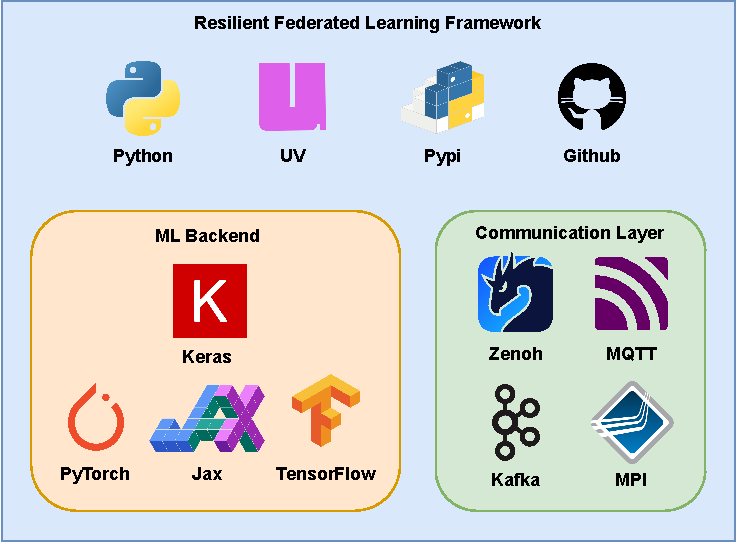
\includegraphics[width=0.8\textwidth]{figs/technology-stack.pdf}
    \caption[Software Stack of the Resilient FL Framework]{Diagram presenting the key software components comprising the Resilient \ac{fl} Framework, including core development tools, interchangeable \ac{ml} backends, and diverse communication protocols, emphasizing its modular design.}
    \label{fig:technology-stack}
\end{figure}

The implementation of the proposed framework is built primarily using Python. This choice was motivated by Python's widespread adoption and robust ecosystem within the data science and \ac{ml} communities, offering a balance of ease of use and performance through highly optimized libraries, as highlighted by \citeauthor{raschka2020machine} in their survey of the field \cite{raschka2020machine}.

For effective management of project dependencies and ensuring reproducible development environments, crucial for any substantial software project, we used UV~\footnote{\url{https://docs.astral.sh/uv/}}. UV is an extremely fast Python package and project manager, written in Rust. It is known for its significant speed advantages over traditional tools like pip and aims to consolidate the functionality of multiple tools (such as pip, pip-tools, and virtualenv) into a single, efficient utility. UV provides comprehensive features including dependency resolution, package installation, virtual environment creation, and even Python version management, making it a powerful choice for streamlining the development workflow. 

Version control is indispensable for tracking changes, collaborating, and maintaining a software project's history. Git was employed for this purpose, with the framework's codebase hosted on GitHub~\footnote{\url{https://github.com/leoalmPT/FlexFL}}. The choice of GitHub aligns with industry standards and best practices for software development, ensuring that the project is accessible to contributors and users alike. The publicly available repository allows for transparency and community engagement in the development process.

The implemented framework is available as a standard Python package on the \ac{pypi} to facilitate easy access and distribution for other researchers and practitioners. This availability allows users to effortlessly install the framework and its dependencies using simple commands (e.g., \texttt{pip install flexfl}), providing both a Python library for programmatic use and a \ac{cli} tool for direct execution and experimentation, contributing to the goal of making the framework an open-source resource.

For the core \ac{ml} operations, the framework needed to integrate with established \ac{ml} libraries. While several powerful libraries exist, TensorFlow, PyTorch, and JAX are currently among the most widely used in the Python ecosystem for deep learning and numerical computation. These libraries, however, differ significantly in their \acp{api}, design philosophies, and typical use cases. As mentioned in Chapter~\ref{chap:proposed_solution}, the ML Backend module of our framework is designed specifically to abstract away these differences, providing a consistent interface for the rest of the system regardless of the underlying \ac{ml} library. 

In this implementation, we have built support primarily around Keras, a high-level \ac{api} that acts as a powerful abstraction layer. The Keras philosophy emphasizes that it is a deep learning \ac{api} designed with a focus on debugging speed, code elegance and conciseness, maintainability, and deployability. Crucially, Keras achieves this while offering a multi-backend approach, giving users the freedom to work with JAX, TensorFlow, and PyTorch, and allowing them to build models that can move seamlessly across these frameworks and leverage the strengths of each ecosystem. Additionally, we have also integrated support for TensorFlow and PyTorch directly, allowing users to choose the backend that best fits their needs. This flexibility is essential for researchers and practitioners who may have specific requirements or preferences for their \ac{ml} workflows.

Moving to the communication infrastructure, a critical component for coordinating clients and the server in a distributed setting, we implemented support for all four protocols discussed in Chapter~\ref{chap:background}: \ac{mpi} (via Open \ac{mpi}), \ac{mqtt}, Kafka, and Zenoh. While \ac{mpi} may not be ideally suited for the dynamic network environments inherent in \ac{fl} due to its reliance on static configurations and lack of built-in fault tolerance for node failures, its inclusion serves as a valuable benchmark for performance comparison, given its prevalence and optimization for speed in \ac{hpc} environments. 

The implementation of \ac{mqtt}, Kafka, and Zenoh, on the other hand, allows the framework to leverage protocols better designed for dynamic and potentially unreliable networks, offering flexibility and enabling empirical evaluation of their performance and the framework's resilience mechanisms under conditions with and without worker failures or disconnections.



\section{Federated Learning Algorithms}
\label{sec:federated-learning-algorithms}

Building upon the architectural principles established in Chapter~\ref{chap:proposed_solution} and the algorithmic taxonomy discussed in Chapter~\ref{chap:background}, our framework implements the four primary types of \ac{fl} algorithms to demonstrate versatility and evaluate performance across different collaboration and scheduling paradigms. These are Centralized Synchronous, Centralized Asynchronous, Decentralized Synchronous, and Decentralized Asynchronous algorithms. Each algorithm is designed to operate within the framework's modular architecture, allowing for easy integration and experimentation with various components.

These standard algorithmic implementations incorporate several key adaptations and features beyond their basic theoretical descriptions to address the objectives of resilience and modularity in dynamic network environments. These are discussed in detail in this section.

\subsection{Dynamic Worker Pool and Epoch Definition}
\label{sec:dynamic-worker-pool}

A core adaptation, facilitated by the Worker Manager module, is managing a dynamic pool of potential workers. Instead of assuming a fixed set of participating devices, the framework dynamically selects a \texttt{subpool} of available and suitable workers at the start of each training round or epoch. This allows devices to join or leave the network seamlessly without disrupting the training process, contributing directly to elasticity and resilience.

Within our framework, a training \texttt{epoch} or \texttt{round} represents a complete cycle of global model coordination and update involving the selected worker subpool. A key parameter governing this process is the concept of \texttt{iterations} per epoch for Synchronous approaches. This defines the number of times that the parameter server sends tasks to the workers and collects their updates. The definition of epochs and iterations depends on the algorithm type:

\begin{itemize}
    \item \textbf{Centralized Approaches:} The primary task for each worker in a round is to receive the current global model, compute gradients on a local mini-batch, and send these gradients to the Parameter Server. The total number of effective computations (tasks) in a round is thus related to the sum of the number of batches processed by all selected workers. The number of iterations is defined by the total number of tasks divided by the number of workers in the subpool. 
    \item \textbf{Decentralized Approaches:} Each worker's task in a round involves performing a specified number of local epochs and then exchanging their resulting local model or parameters with the parameter server. One global synchronization round corresponds to each selected worker completing their local training phase and submitting their updates. Only 1 iteration is performed per round.
\end{itemize}

\subsection{Resilience Mechanisms}
\label{sec:resilience-mechanisms}

Regardless of the algorithm type, the framework implements resilience mechanisms to handle worker failures and disconnections. These mechanisms are designed to ensure that the training process can continue despite unexpected disruptions, aligning with the framework's goal of resilience in dynamic network environments.

In Asynchronous algorithms, where the system can tolerate some delays, the framework monitors the progress of tasks assigned to workers in the worker subpool. If a worker fails, disconnects, or becomes unresponsive while executing its task (either gradient computation in centralized async or local training in decentralized async), the Worker Manager detects it. 

The task associated with the failed worker can then be automatically rescheduled and assigned to another available worker from the dynamic pool, according to the scheduling policy, ensuring that the necessary contribution for the round is eventually completed. If the number of workers drops below a certain threshold, the Parameter Server will pause the training round by stopping the distribution of new tasks until the Worker Manager detects that enough workers are available again.   

Synchronous algorithms inherently require a higher degree of coordination. To prevent single stragglers or failures from halting the entire training process, a configurable completion threshold (e.g., 50\%) is introduced for each iteration. If the number of workers in the selected worker subpool that successfully complete and submit their tasks meets or exceeds this threshold, the Parameter Server proceeds with the aggregation step using the available updates. This allows the training to advance even if a subset of workers fails or is significantly delayed.

\subsection{Optimizations}
\label{sec:optimizations}

Several optimizations have been incorporated into the framework to enhance its efficiency and scalability, particularly in handling large models and coordinating multiple workers.

A key optimization concerns aggregating model weights or gradients received from workers on the Parameter Server. To conserve memory and avoid the need to store the whole model or gradient updates from every worker simultaneously, the aggregation process is performed on the fly. As updates arrive from individual workers, they are incrementally incorporated into a running weighted sum or average. This allows the memory associated with a worker's update to be released immediately after it has been processed. 

For instance, if $M$ represents the size of a single model update and there are $N$ workers, this approach reduces the server's peak memory footprint from potentially $N \times M$ bytes (if all updates were buffered simultaneously) to approximately $2 \times M$ bytes (for the current global model and one incoming update). This significantly enables support for a larger number of workers or larger model sizes than would otherwise be possible.

Furthermore, to minimize idle time and increase overall throughput, the framework optimizes the timing of task distribution to workers. Instead of waiting for the Parameter Server to complete the full validation process on the newly updated global model, tasks for the next round can be initiated as soon as the global model state is mathematically finalized by the aggregation process. This helps to pipeline the training process, reducing the latency between rounds. 

For example, if validation for each epoch takes $T$ seconds and the training runs for $E$ epochs, this optimization can reduce the total training time by up to $E \times T$ seconds by overlapping validation with the start of the subsequent round, thereby improving the utilization of both the server and worker resources, especially when the Parameter Server is not a bottleneck.

Additionally, a crucial change for asynchronous approaches was made. With dynamic worker participation, we must ensure that workers train on models that do not excessively lag behind the global model. In the original decentralized asynchronous algorithms, model differences were used for updates, but this is not suitable when workers might skip rounds due to the dynamic pool selection. To address this, at the start of each round, the Parameter Server sends the current global model to all workers in the current subpool, and each worker then performs their tasks using this model. This ensures that, despite the asynchronous nature and potential for variable participation, workers start their local computations from a recent common reference point, which helps convergence stability.



\section{Additional Features}
\label{sec:additional-features}

Beyond the core modular architecture and implemented \ac{fl} algorithms, the framework provides a suite of additional features, primarily exposed through \ac{cli} tools. These tools are designed to streamline the entire Federated Learning workflow, from data preparation and setup to experimentation, simulation, and analysis, making the framework more accessible and practical for researchers and practitioners. 

The primary \ac{cli} commands available are:

\begin{itemize}
    \item \texttt{flexfl}: This is the main command for executing \ac{fl} experiments. It provides extensive configuration options through command-line arguments to define the setup of all seven core modules of the framework, enabling flexible experimentation with different algorithm types, communication protocols, ML backends, datasets, and more. Details on the argument parser and configuration options will be provided later in Section~\ref{sec:technical-details}.
    \item \texttt{flexfl-preprocess}: Used to manage the dataset preparation process. This command facilitates the downloading and initial preprocessing of datasets, allowing users to prepare data for specific experiments or batch-process multiple datasets supported by the framework's Dataset Manager module.
    \item \texttt{flexfl-division}: Handles the division of datasets for distributed training. This command splits processed datasets into training, validation, and testing sets. Crucially for \ac{fl}, it also partitions the training data among a specified number of workers, supporting both \ac{iid} and \ac{non-iid} data distributions to simulate various real-world scenarios encountered in \ac{fl}.
    \item \texttt{flexfl-benchmark}: Provides tools for benchmarking communication performance and resilience of the network layer. Designed to be run typically on two nodes (one acting as a server, one as a worker), this command allows for testing specific communication protocols implemented in the Communication Layer, simulating basic worker failures, and measuring the time required to send and receive payloads of varying sizes multiple times between nodes.
    \item \texttt{flexfl-res}: A utility specifically for simulating worker resilience under failure conditions. This command launches a specified process (e.g., a worker instance) and introduces controlled disruptions by randomly killing and restarting the process based on configurable probabilities and time intervals. This tool is helpful for empirically testing the fault tolerance mechanisms integrated into the framework under realistic failure scenarios.
    \item \texttt{flexfl-plot}: Dedicated to visualizing experiment results and system performance, this command processes the structured logs generated by framework runs and automatically generates various data visualizations, including plots and tables, for analyzing key metrics such as communication times, worker computation times, worker timelines, size of exchanged payloads, and overall run duration. This aids in understanding performance characteristics and the impact of different configurations.
\end{itemize}

These \ac{cli} tools collectively provide a comprehensive environment for setting up, running, simulating, and analyzing \ac{fl} experiments with the proposed framework, facilitating both research and practical application. But while these tools provide the interface for configuring and running \ac{fl} experiments on individual nodes, conducting realistic distributed and \ac{fl} studies requires managing a cluster of interconnected machines. 

To address the complexities of creating, configuring, and managing a fleet of \acp{vm} for experimentation, a separate package named \texttt{pxm-tools} and also available on \ac{pypi} was created. This tool leverages the Proxmox Virtual Environment \ac{api}, a widely used open-source platform for virtualization management. \texttt{pxm-tools} provides a command-line interface designed for ease of use when performing bulk operations on \acp{vm}. 

Its core functionalities include easily creating, editing, removing, starting, and stopping multiple \acp{vm} simultaneously. It also offers flexible configuration by allowing any argument available through the Proxmox \ac{api} to be set during \ac{vm} creation or editing. This is crucial for simulating diverse and heterogeneous environments by configuring \ac{vm} resources like the number of CPU cores, RAM size, storage, and critically, network interface bandwidth limits. The ability to control network conditions is essential for evaluating the framework's resilience under varying real-world constraints. 

Furthermore, \texttt{pxm-tools} automatically retrieves necessary \ac{vm} information, such as their unique IDs and assigned IP addresses, which are vital for subsequent interaction and logging. By abstracting the direct interaction with the Proxmox \ac{api} into simple \ac{cli} commands, \texttt{pxm-tools} significantly simplifies the process of setting up and tearing down experimental clusters, enabling rapid iteration and evaluation cycles.

Once the experimental \acp{vm} are provisioned and configured using \texttt{pxm-tools}, an efficient method is needed to interact with all or a subset of these machines collectively. Custom scripts were developed to enable parallel execution of commands across the chosen \acp{vm}, leveraging \ac{ssh} for secure communication. 

These scripts are designed to streamline the experimental workflow by allowing users to execute arbitrary shell commands concurrently on all selected \acp{vm}, drastically reducing the time required for setup tasks like installing dependencies or configuring the environment. They also efficiently distribute the preprocessed and partitioned datasets (prepared using \texttt{flexfl-division}) to the corresponding worker \acp{vm}, ensuring each node receives its designated data split for the experiment, and gather experimental outputs, such as logs, performance metrics, and final models, from all participating \acp{vm} in parallel after a run is complete. 

Finally, these scripts can launch the main \texttt{flexfl} command on the designated server \ac{vm} and all selected worker \acp{vm} simultaneously to initiate a distributed training run. These parallel interaction scripts, combined with \texttt{pxm-tools}, provide a complete toolchain for managing the experimental environment and executing Federated Learning experiments at scale on a cluster of \acp{vm}, crucial for thoroughly evaluating the framework's performance and resilience.



\section{Technical Details}
\label{sec:technical-details}

This section delves into the technical intricacies of the framework's implementation, focusing on key aspects such as the communication layer protocols, the worker scheduling policy, the functionality of the Worker Manager, early stopping mechanisms, the configuration interface via the argument parser and optional libraries, how experimental results are saved, and guidelines for extending the framework. These details highlight the practical realization of the modular and resilient design principles discussed in Chapter~\ref{chap:proposed_solution}.

\subsection{Communication Protocols}
\label{sec:comm-protocols-caveats}

As discussed in Chapter~\ref{chap:background}, the framework implements support for multiple communication protocols (Zenoh, \ac{mqtt}, Kafka, and \ac{mpi}) to offer flexibility and adaptability to diverse network environments. While the Communication Layer module provides a consistent \texttt{send} and \texttt{recv} interface to the rest of the framework, there are protocol-specific nuances and implementation details, particularly regarding asynchronous operation and fault detection.

All supported protocols require an initial connection phase where workers register with the Parameter Server to obtain a unique identifier and establish communication channels. The implementations for Zenoh and  \ac{mqtt} leverage their native support for asynchronous message handling, typically through threading or event loops, and include built-in capabilities to detect client disconnections (e.g., via callbacks or subscription mechanisms). This native support simplifies the implementation of resilience features dependent on knowing worker connection status.

Kafka, in contrast, is optimized for high-throughput, persistent message streaming and lacks native real-time disconnection notifications without incurring significant partition rebalancing overhead, which is undesirable in a dynamic \ac{fl} setting. To overcome this, the Kafka implementation required a manual heartbeat mechanism, where workers periodically send health check messages to the server. 

\ac{mpi}, being primarily designed for synchronous, blocking communication in high-performance computing environments, inherently operates in a request-response manner. But, as previously mentioned, it lacks built-in capabilities to detect client disconnections directly at the protocol level without explicit application-level checks, which imposes constraints on handling dynamic worker pools compared to the other protocols.

\subsection{Worker Scheduling Policy}
\label{sec:worker-scheduling-policy}

The framework incorporates a worker scheduling policy that is responsible for selecting the subset of available workers participating in each training round or epoch. The currently implemented policy is Round Robin, a well-established \cite{rasmussen2008round}, simple, and fair scheduling approach that cycles through the pool of available workers. In our dynamic setting, the Round Robin scheduler selects workers sequentially from the currently connected pool at the start of each round.

A key advantage of the framework's modular design is that the scheduling policy is encapsulated within the \ac{fl} algorithm. This allows users to easily replace the default Round Robin implementation with alternative policies (e.g., based on worker capabilities, data distribution, historical performance, or network conditions) to suit specific requirements, without needing to modify other core components of the framework. The scheduler's integration with the dynamic worker pool management enables seamless adaptation to workers joining or leaving the training process.

\subsection{Worker Manager}
\label{sec:worker-manager}

The Worker Manager is a pivotal module for achieving resilience and abstracting the complexities of dynamic worker participation from the core \ac{fl} algorithms. It acts as the central coordinator on the Parameter Server and also runs a client-side component on each worker. Its core functionalities include managing the list of currently connected workers and the selection of the worker subpool for each round, effectively hiding the complexities of workers joining or leaving from the \ac{fl} algorithm logic. 

Users can configure custom callbacks for key events, such as when a new worker joins the system (executable on both the Parameter Server and the joining worker) or  when a worker disconnects or fails (primarily handled on the Parameter Server). These callbacks allow for custom logic to be executed during these events, enhancing flexibility.

Communication within the framework is structured using message types (e.g., work, work\_done). that the user specifies when sending messages. The Worker Manager facilitates flexible message reception by allowing users to register callbacks to be executed automatically when a message of a specific type is received, which enables asynchronous processing of incoming messages. 

Users can also perform blocking receives for messages of a specific type, waiting until a message of that type arrives. Furthermore, the framework allows for the combination of blocking receives with callbacks. During a blocking wait for a specific message type, the Worker Manager can process other incoming messages in the background using their registered callbacks, such as join messages.

Integrated with the message handling, the Worker Manager monitors blocking receive operations for worker failure detection and rescheduling. If a worker fails or disconnects while a blocking receive is pending for a task assigned to it, the Worker Manager can trigger a user-defined callback that allows for the implementation of task rescheduling logic, enabling the framework to assign the failed task to another worker.

Messages received in the background that do not have an immediate callback registered are stored in an internal queue, so blocking receive operations first check this queue before waiting for new messages from the communication layer, ensuring that already received messages are processed promptly. The manager can also store relevant metadata for each connected worker, regarding the \ac{fl} training or potentially performance metrics, which can be used by scheduling policies or custom callbacks.

Finally, the Worker Manager provides a mechanism for conditional waiting, allowing the process to wait for a specific condition (defined by a callback function) to become true while the manager continues to process incoming messages in the background. This is useful for coordinating actions that depend on the state of multiple workers or received messages.

Figure~\ref{fig:worker-manager} presents a detailed flow diagram that illustrates how incoming messages are processed, how callbacks enable asynchronous handling and how the internal queue manages background messages, underscoring the robust communication pipeline designed to support the framework's operations under challenging conditions.

\begin{figure}[!htbp]
    \centering
    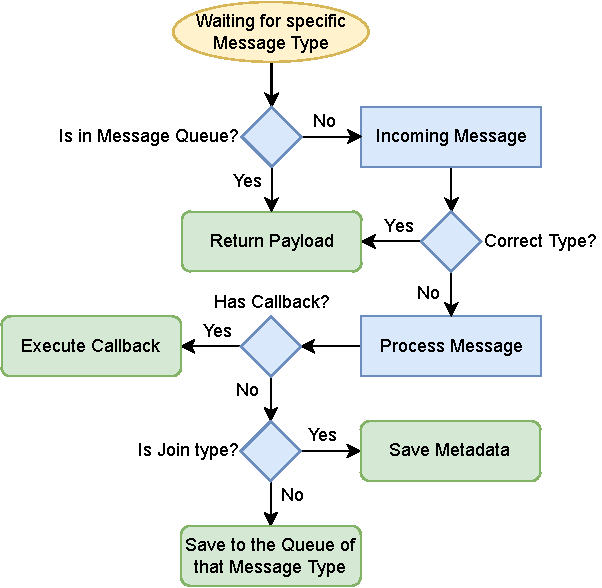
\includegraphics[width=0.7\textwidth]{figs/worker-manager.pdf}
    \caption[Worker Manager Message Processing Flow]{Flow diagram illustrating the Worker Manager's message processing, callback handling, and internal queue management.}
    \label{fig:worker-manager}
\end{figure}

\subsection{Early Stopping}
\label{sec:early-stopping}

To prevent overfitting and optimize training time, the framework implements an early stopping mechanism controlled on the Parameter Server. This feature allows users to define criteria for halting the training process based on the model's performance on a validation set. Configurable parameters include \texttt{patience}, \texttt{delta}, \texttt{target\_score}, and the \texttt{main\_metric} used for evaluation. 

The validation is performed at the end of each epoch or round using the current global model. If the monitored metric's value meets or exceeds the target score (e.g., achieving a certain accuracy level) or if the metric has not improved by at least delta for patience consecutive validation checks, the Parameter Server signals all participating workers to stop training, and the experiment concludes. The interpretation of ''improvement'' depends on the metric: in general, for classification problems, higher metric values (closer to 1) are generally better, while for regression problems, lower values (closer to 0) indicate better performance. 

In each epoch, the model state corresponding to the best-achieved metric value seen so far is automatically saved. Upon termination, regardless of whether early stopping was triggered or the maximum number of epochs was reached, the framework automatically loads and provides the best model for further analysis or deployment.

\subsection{Argparser and Optional Libraries}
\label{sec:argparser}

The framework's flexibility and modularity are heavily supported by a sophisticated configuration system, primarily accessed through the main \texttt{flexfl} \ac{cli} command. This system uses a powerful argument parser that allows users to specify the desired configuration for every aspect of the \ac{fl} experiment, including selecting specific implementations for each of the seven core modules (ML Backend, FL Backend, Communication Layer, etc.) and providing their module-specific arguments. Configuration can be provided directly via command-line arguments or through a configuration file, enabling reproducible setups.

Addressing the challenge of managing a wide array of potential module options and avoiding library conflicts (e.g., between TensorFlow and PyTorch), the argument parser incorporates logic that inspects each module's available Python code implementations dynamically. By analyzing the Python syntax tree of the installed module classes, it automatically identifies configurable constructor arguments and their expected data types. 

This information is used to configure the argument parser dynamically at runtime, ensuring that only valid options are presented and correctly parsed. This dynamic configuration enables lazy loading of module dependencies, so that the required libraries for a chosen module implementation are only imported when that module is actually instantiated, significantly improving startup performance and reducing potential conflicts in environments with multiple large \ac{ml} libraries. A key benefit is that when new module implementations are added by extending the base classes, their constructor arguments are automatically recognized and incorporated by the argparser without requiring manual updates to the configuration system.

\subsection{How Results Are Saved}
\label{sec:results-saving}

Experimental results generated by the framework are systematically organized and saved to facilitate analysis and reproducibility. When an experiment is executed via the \texttt{flexfl} command, a dedicated output folder is created. The name of this folder is determined either by a user-provided name through the argument parser or defaults to a timestamp representing the start time of the Parameter Server process, ensuring unique identification for each run. 

Several subdirectories and files are stored within this root experiment folder. For perfect reproducibility, a file containing the exact configuration arguments used for the run is saved. The best model checkpoint (as determined by the early stopping criteria or the final model if early stopping is disabled) is saved in a dedicated location. Furthermore, for each node (Parameter Server and each Worker) involved in the experiment, a subfolder named after the node's identifier is created. 

Inside each node's folder, a comprehensive log file is generated in \ac{jsonl} format. This log file captures a rich stream of events and data throughout the experiment, including timestamps for send and receive operations, details about exchanged payloads, epoch-level training and validation metrics (loss, accuracy, etc.), worker computation times, and other relevant system events. This structured \ac{jsonl} format allows subsequent analysis using external tools, as supported by the \texttt{flexfl-plot} utility.

\subsection{How to Extend the Framework}
\label{sec:framework-extension}

Extending the framework with new implementations for any of the seven core modules is designed to be straightforward, leveraging the modular architecture and Python's object-oriented capabilities. The framework provides a set of abstract built-in base classes, with one abstract class defined for each core module type. 

To add a new implementation, a user simply needs to create a new Python class that inherits from the corresponding abstract base class, which defines a set of required methods (interfaces) that the new implementation must provide. The user then writes the code for their specific algorithm, protocol, or component within these methods, adhering to the defined interfaces. 

Once the new class is implemented, it becomes discoverable by the argument parser due to its dynamic inspection capabilities. This design ensures that adding new capabilities does not require modifying the core framework logic, promoting clean separation of concerns and fostering community contributions and customization.

\chapter{Evaluation}
\label{chap:evaluation}

\begin{introduction}

A series of experiments was designed and conducted in a controlled environment to rigorously assess the performance, resilience, and modularity of the proposed Resilient Federated Learning Framework. This chapter details the experimental setup, the datasets and models used, the metrics measured, the various experimental scenarios investigated, and the results and analysis for each scenario.

\end{introduction}

\section{Experimental Setup}
\label{sec:experimental-setup}

The experimental setup was designed to emulate scenarios involving resource-constrained client devices participating in a federated training process coordinated by a more powerful central server. This mirrors typical edge computing \ac{fl} use cases where client devices (like mobile phones or \ac{iot} devices) have limited computational resources and unstable network connectivity compared to a central server or cloud instance. 

The experiments were conducted on a cluster of \acp{vm} running on underlying ARM-based hardware, specifically the HUAWEI Kunpeng 920 7260 processor\footnote{\url{https://www.hisilicon.com/en/products/kunpeng/huawei-kunpeng/huawei-kunpeng-920}},  with Ubuntu 24.04 LTS as the guest operating system. This cluster was hosted on a Proxmox server, which provided a flexible and efficient virtualization environment. 

The cluster configuration for the experiments included a single \ac{vm} designated as the Parameter Server, configured with 8 CPU cores and 16 GB of RAM, providing significantly more resources than the worker \acp{vm}, and with a network interface configured with a maximum bandwidth of approximately 5 GBps, simulating a high-capacity central node connection. This configuration ensured that the Parameter Server could handle the computational load of aggregation and avoid becoming a network bottleneck, allowing us to focus on communication challenges between the server and the workers.

To represent different client populations, two sets of worker \acp{vm} were used. The first, a uniform worker set, consisted of 10 \acp{vm}, each configured identically with 2 CPU cores and 4 GB of RAM, and a network interface bandwidth cap of 50 Mbps, simulating typical broadband or limited wireless connections for client devices. 

The second, a heterogeneous worker set, was configured with varying specifications for CPU cores, RAM, and network bandwidth caps across the 30 \acp{vm} to simulate a diverse population of client devices with heterogeneous capabilities. This worker set consists of 6 groups of 5 \acp{vm} with varying CPU cores (2, 4, and 6), RAM (4, 6, and 8 GB), and network bandwidth (50, 75, and 100 Mbps). 

Finally, accurately measuring communication times and synchronization events is vital for assessing the framework's performance and resilience. To ensure this, precise clock synchronization was essential across all participating nodes. The parameter server \ac{vm} was configured to act as an \ac{ntp} server, with all worker nodes synchronized to it. This setup minimized time drift between machines, allowing for the reliable calculation of communication latencies and event timestamps throughout the experiments.

Figure~\ref{fig:experimental-setup} illustrates the described experimental setup, showing the configuration of the Parameter Server and the two worker sets.

\begin{figure}[!htbp]
    \centering
    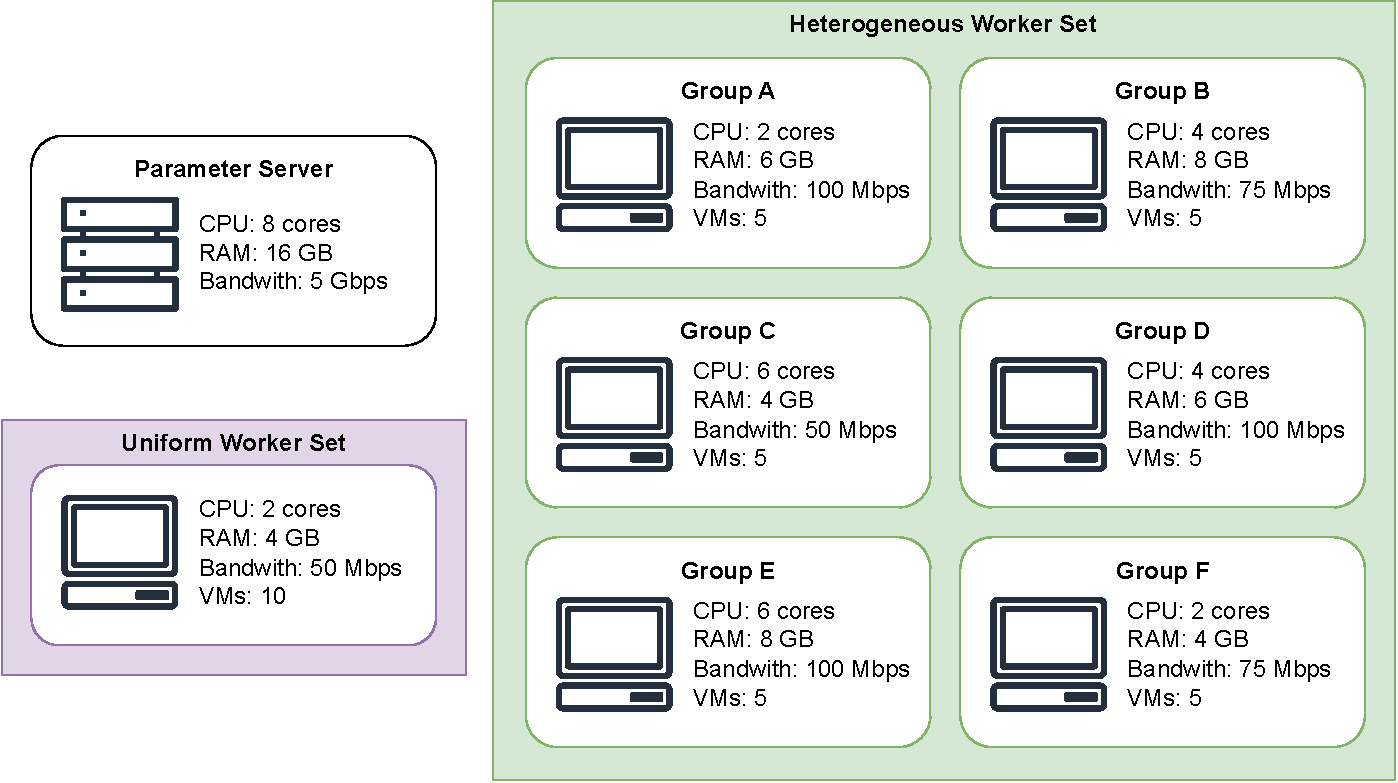
\includegraphics[width=\textwidth]{figs/vms.pdf}
    \caption[FL Testbed Configuration]{Illustration of the experimental setup, detailing the central Parameter Server and the two distinct sets of worker \acp{vm}: a uniform worker set with 10 \acp{vm}, and a heterogeneous worker set with 30 \acp{vm} comprising multiple groups with varying resource configurations.}
    \label{fig:experimental-setup}
\end{figure}


\section{Datasets and Models}
\label{sec:datasets-and-models}

Effective evaluation of a \ac{fl} framework requires careful selection of datasets and models relevant to its intended real-world applications. \ac{ids} and \ac{iot} environments stand out as highly practical and pertinent domains for \ac{fl} implementation. This is primarily due to the critical need for data privacy and security, alongside the inherent distributed nature of data sources in these settings. Training robust \ac{ids} models often necessitates access to sensitive data, like network traffic or device information, which is challenging or impossible to centralize \cite{10608461}.

\ac{fl} presents a viable solution by enabling collaborative model training among participants without requiring the sharing of raw data. Evaluating our framework within the context of \ac{ids} and \ac{iot} enables us to demonstrate its capabilities in scenarios that directly reflect these practical constraints and opportunities.

While well-established datasets like KDD98~\cite{kdd98}, KDDCUP99~\cite{kdd99}, or NSLKDD~\cite{nslkdd} exist for training \ac{ids} models, they are widely regarded as outdated and not fully representative of today's network traffic, as detailed in~\cite{kostas2023iotgem}. This significantly restricts their applicability to contemporary network security research. Considering this limitation, we decided to use two recent and widely-recognized state-of-the-art datasets, UNSW-NB15~\cite{unswnb15} and ToN-IoT~\cite{toniot}, which better capture current network threats and reflect \ac{iot} environments.

\subsection{UNSW-NB15}
\label{sec:unsw-nb15}

The UNSW-NB15 dataset is synthetically generated from the \ac{accs}. It combines real modern regular network traffic with synthesized contemporary attack activities. The dataset comprises over 2 million records, each with 49 features, and is suitable for both binary and multi-class classification tasks. Malicious activities are labeled with one of nine specific attack categories: \ac{dos}, Analysis, Backdoor, Exploits, Fuzzers, Generic, Reconnaissance, Shellcode, and Worms.

To avoid complex preprocessing procedures, in this study, we used the NF-UNSW-NB15\footnote{\url{https://espace.library.uq.edu.au/view/UQ:ffbb0c1}} preprocessed dataset published in~\cite{nfunswnb15} by the University of Queensland. This dataset version incorporates the same data as the original but standardizes features using NetFlow. NetFlow is a widely adopted Cisco protocol for collecting IP traffic information and monitoring network flow (e.g., total bytes transferred, number of packets, duration). The creators of this version state that their motivation was the lack of a standard feature set commonly found in general \ac{ids} datasets.

Following prior work on this dataset, specifically~\cite{abou2020evaluation}, which investigated various \acp{nn} including \ac{ann}, \ac{cnn}, and \ac{rnn} and found them to achieve similar results, we selected the \ac{ann} model. The \ac{ann} strikes a good balance between performance and computational efficiency, making it a suitable choice for potentially resource-limited \ac{fl} workers. However, this \ac{ann} model is rather small, in \cite{abou2020investigating} the authors used a larger model that we considered a better fit for our experiments. 

The \ac{ann} model used in this study consists of three hidden layers (300, 100, and 50 neurons) using the \ac{relu} activation function and a softmax for the output layer as shown in Figure~\ref{fig:unws_nn}. 

\begin{figure}[!htb]
    \centering
    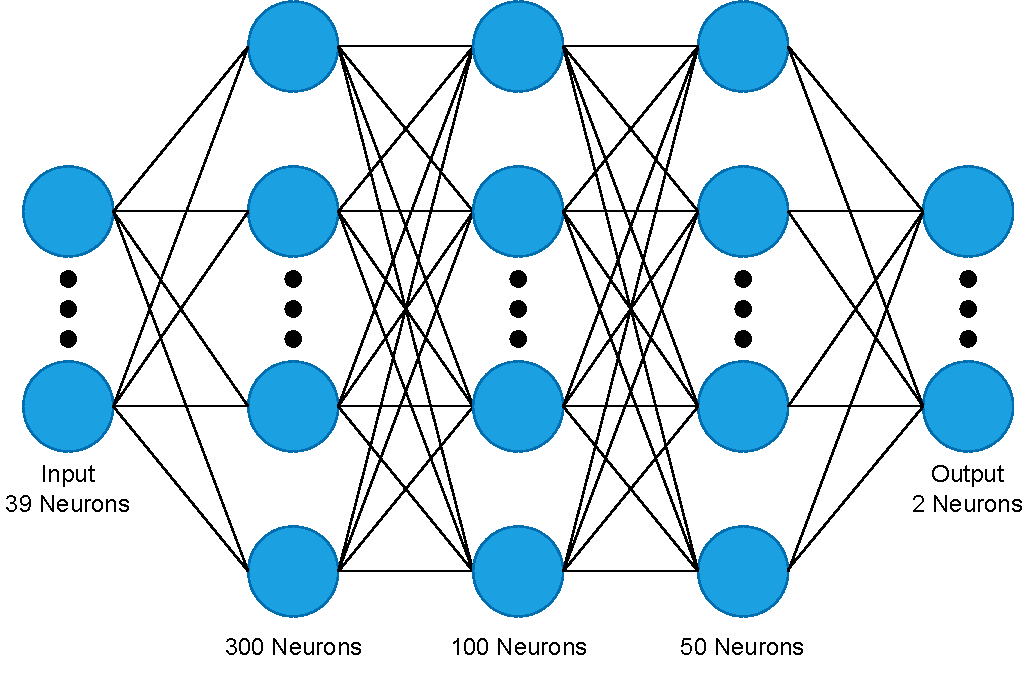
\includegraphics[width=0.8\textwidth]{figs/unsw_nn.pdf}
    \caption[UNSW-NB15 dataset model architecture]{Architecture of the ANN model used for the UNSW-NB15 dataset, consisting of three hidden layers with 300, 100, and 50 neurons, respectively.}
    \label{fig:unws_nn}
\end{figure}

\subsection{ToN-IoT}
\label{sec:ton-iot}

The ToN-IoT is a heterogeneous dataset created by the  \ac{accs} and released in 2019, specifically designed to include telemetry data from an \ac{iot} network. Generated on a realistic testbed, it provides various traces of \ac{iot} services, network traffic, and operating system logs. The dataset contains over 13 million samples and numerous attack scenarios, including Backdoor, \ac{dos}, \ac{ddos}, Injection, \ac{mitm}, Password, Ransomware, Scanning, and \ac{xss}. Like UNSW-NB15, ToN-IoT supports both multi-class attack classification and binary normal/malicious classification.

For this study, we used the NetFlow version of the ToN-IoT dataset, NF-ToN-IoT\footnote{\url{https://espace.library.uq.edu.au/view/UQ:38a2d07}}, published by the same authors as the NF-UNSW-NB15 dataset.

Based on the model evaluations for the ToN-IoT dataset presented in~\cite{kumar2021p2idf}, which compared a \ac{sae} and an \ac{ann} model, we selected the \ac{ann} model. The \ac{ann} architecture used for this dataset features two hidden layers with 32 and 16 neurons, respectively, also employing the \ac{relu} activation function and a softmax for the output layer. Dropout layers with a rate of 0.2 were included after each hidden layer. The model was trained using the Adam optimizer, mirroring the approach in the cited paper.

This model is smaller than the one used for UNSW-NB15, allowing it to exhibit distinctive characteristics and ensuring that the experiments are not biased by the model size. The architecture of the \ac{ann} model used for the ToN-IoT dataset is shown in Figure~\ref{fig:ton_nn}.

\begin{figure}[!htb]
    \centering
    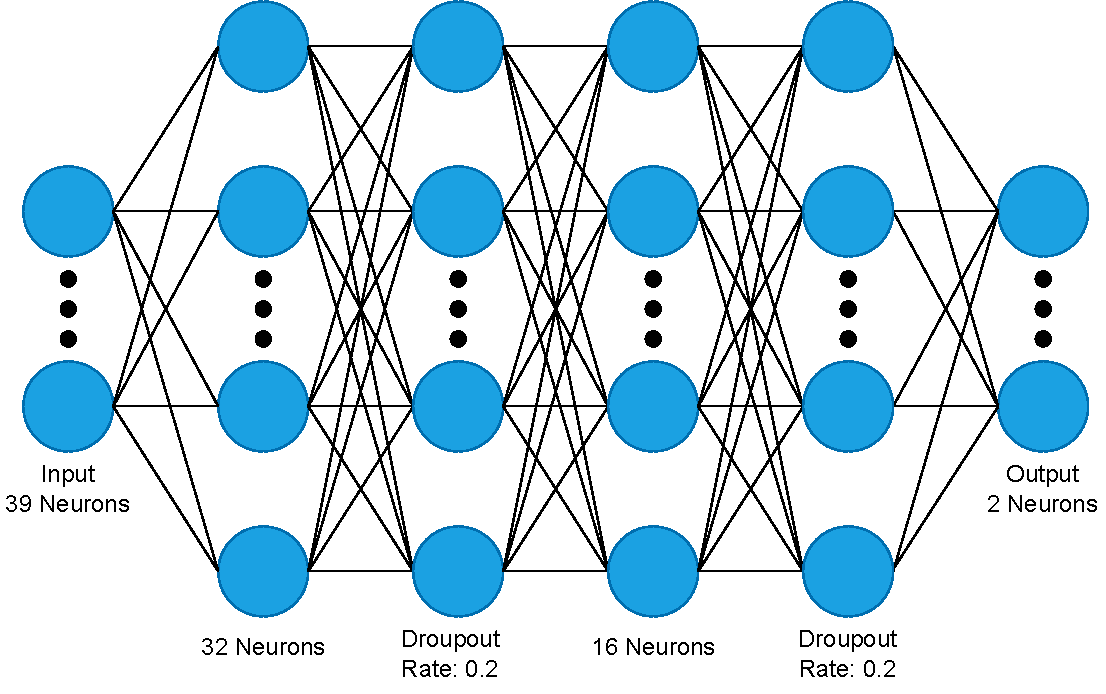
\includegraphics[width=0.9\textwidth]{figs/ton_nn.pdf}
    \caption[ToN-IoT dataset model architecture]{Architecture of the ANN model used for the ToN-IoT dataset, consisting of two hidden layers with 32 and 16 neurons, respectively, with dropout layers in between.}
    \label{fig:ton_nn}
\end{figure}

\subsection{Data Division}
\label{sec:data-division}

Our experiments focused on the binary classification task using the UNSW-NB15 and ToN-IoT datasets, aiming to train models that can distinguish between normal and malicious network traffic. To prepare the data for the distributed training process, we first preprocessed the datasets, without data normalization, and split them into three primary partitions: a training set (70\%), a validation set (15\%), and a testing set (15\%) for the UNSW-NB15 dataset, and a training set (90\%), a validation set (5\%), and a testing set (5\%) for the ToN-IoT dataset, because this dataset is significantly larger than UNSW-NB15 (over 13 million samples compared to UNSW-NB15's 2 million). This division ensures that the model can be trained effectively while also being evaluated on unseen data.

The training data were then partitioned among the workers participating in each experiment's subpool according to specific distribution strategies, primarily \ac{iid}, achieved by globally shuffling the dataset and distributing equal-sized partitions to each worker. A critical aspect of this data handling, consistent with the principles of \ac{fl} and preserving data privacy, is that each worker node performed data normalization (e.g., scaling features) using only the statistics (such as mean and standard deviation) derived from its own local data split, without sharing raw data or statistics with other nodes or the Parameter Server.

In this \ac{fl} setup, the validation set was used by the parameter server for periodic evaluation of the global model's performance throughout the training process. It is important to note that, for our experiments, the validation data was not used to influence the aggregation mechanism or global model updates, thereby ensuring the reported metrics effectively represent the model's generalization performance on unseen data, akin to a test set. The remaining testing sets were reserved for future evaluation of the final trained model's performance on unseen data.

Furthermore, the resilience mechanisms integrated into the system, such as handling client dropouts, do not alter the aggregation logic or influence the model update process. This ensures consistency and integrity in the training dynamics. Nonetheless, the modular design of the FL Backend does allow for future integration of validation-aware aggregation strategies. 




\section{Metrics}
\label{sec:metrics}


Rigorous evaluation of a \ac{ml} framework, particularly one designed for distributed and potentially unreliable environments like \ac{fl}, needs a comprehensive set of metrics. These metrics fall into two main categories: standard \ac{ml} performance metrics and system-level metrics derived from detailed logging.

Regarding the \ac{ml} performance, the specific metrics evaluated depend on the type of task being performed (classification or regression) and the loss function used. For the binary classification tasks utilizing the UNSW-NB15 and ToN-IoT datasets in this study, the following standard classification metrics are evaluated: \ac{mcc}, Accuracy, and F1-score \cite{chicco2020advantages, diallo2024machine}. They serve as primary indicators of the model's learning progress, convergence, and final quality.

Accuracy provides the overall proportion of correct predictions, while the F1-score offers a balanced view of precision and recall, which is particularly important for tasks like intrusion detection, where both minimizing false positives and false negatives is crucial. \ac{mcc} is a single-value metric that measures the quality of binary classifications, particularly useful for imbalanced datasets. It takes into account all four values in the confusion matrix: \ac{tp}, \ac{tn}, \ac{fp}, and \ac{fn}. It is calculated as:

\begin{equation}
    \text{MCC} = \frac{\text{TP} \cdot \text{TN} - \text{FP} \cdot \text{FN}}{\sqrt{(\text{TP} + \text{FP})(\text{TP} + \text{FN})(\text{TN} + \text{FP})(\text{TN} + \text{FN})}}
\end{equation}

For completeness and to demonstrate the framework's versatility beyond classification, standard regression metrics such \ac{smape}, \ac{mse}, and \ac{mae} \cite{chicco2021coefficient} are also considered as potential evaluation criteria depending on the model and dataset used. \ac{mse} is the average of the squared differences between predicted and actual values, and \ac{mae} is the average of the absolute differences. \ac{smape} is a measure of prediction accuracy, expressed as a percentage, calculated as:

\begin{equation}
    \text{SMAPE} = \frac{1}{n} \sum_{i=1}^{n} \frac{|y_i - \hat{y}_i|}{|y_i| + |\hat{y}_i|} \times 100
\end{equation}
Where \(y_i\) is the actual value, \(\hat{y}_i\) is the predicted value, and \(n\) is the number of data points.

For this evaluation, we primarily focused on global model validation metrics to assess the framework's overall convergence and generalization capabilities on unseen data, rather than tracking training metrics from individual clients. This choice was made to avoid additional overhead, and more importantly, because local training metrics in a federated setting, especially under \ac{non-iid} data distributions, can be misleading and do not reliably reflect the global model's learning progress. In such scenarios, client-specific metrics often exhibit high variance and are not indicative of the model's ability to generalize, making global validation performance a more meaningful and consistent measure.

In addition to model performance, evaluating the framework's resilience, scalability, and efficiency requires collecting detailed system-level data. As discussed in Section~\ref{sec:results-saving}, the framework generates comprehensive \ac{jsonl} log files for each node (Parameter Server and Workers). 

These logs capture a rich stream of events and data points throughout the experiment, including timestamps for send and receive operations of messages, details about exchanged payloads including size and type, epoch-level training and validation metrics (loss, accuracy, etc.), worker computation times for local training tasks, encode and decode times for messages, events indicating when workers join or leave the network, events indicating when workers fail, and markers for the start and end of the entire training run.

This detailed logging allows for the measurement and analysis of various system performance aspects, including the total run duration of the experiment, the evolution of loss and other \ac{ml} metrics over epochs, the number of messages sent and received and the total payload size exchanged, the total communication time across the network, and the total worker computation time and idle/wait time for both the Parameter Server and workers.

It also allows tracking and quantifying the types and timing of worker failures and their corresponding states during a round. This is crucial because it will enable us to differentiate between failures that halt progress (critical failures) and those that are less disruptive (non-critical failures). This provides empirical evidence for the framework's resilience claim by demonstrating how well it continues to train despite various failure scenarios. A worker's status during a round can be categorized into one of five states:

\begin{enumerate}[label=\roman*)]
    \item \textbf{Idle without fail:} The worker was available and did not experience a failure event while idle waiting for a task or the next round.
    \item \textbf{Worked successfully without failing:} The worker was assigned a local training task, completed it, and successfully communicated its update to the server without experiencing a failure event during this epoch.
    \item \textbf{Failed while idle:} A failure event occurred while the worker was available but not actively performing a local training task or communicating. This is generally less disruptive as no computation result is lost. This is considered a \textbf{non-critical failure} as the worker can rejoin the training process without any loss of contribution.
    \item \textbf{Failed while working:} A failure occurred while the worker actively performed a local training task or communicated their update. This is considered a \textbf{critical failure} as the ongoing computation or communication is interrupted, potentially requiring task reassignment in an asynchronous setting.
    \item \textbf{Failed after working successfully:} The worker completed its local training task and successfully communicated its update, but experienced a failure event afterward, before the start of the next round. This is considered a \textbf{non-critical failure} as the contribution for the current round was successfully made.
\end{enumerate}

These metrics provide insights into convergence speed and stability under different conditions, the impact of worker failures on training progress, communication overhead, and the overall efficiency of the framework. By analyzing these metrics, we can assess the framework's performance in terms of resilience, scalability, and efficiency, as well as its ability to adapt to varying worker capabilities and network conditions.



\section{Experimental Scenarios}
\label{sec:experimental-scenarios}

A series of experimental scenarios was designed and executed to comprehensively assess the performance, resilience, modularity, and scalability of the proposed Resilient Federated Learning Framework. These scenarios evaluate the framework's capabilities under different conditions, focusing on key aspects relevant to real-world \ac{fl} deployments, such as communication efficiency, fault tolerance, and scaling with a dynamic and heterogeneous worker pool. Three primary scenarios were investigated in this evaluation.

\textbf{Scenario 1: Impact of Communication Protocols and FL Algorithms} - This scenario is designed to measure and compare the communication overhead associated with different \ac{fl} algorithms implemented within the framework using the UNSW-NB15 dataset and aims to understand inherent communication costs. This is particularly important for identifying the most efficient approaches in bandwidth-limited environments, which are typical of edge computing scenarios where \ac{fl} is often applied. 

This scenario uses the first set of workers, consisting of 10 \acp{vm} with uniform specifications, connected to the Parameter Server. This setup allows for a controlled environment and better visualization of results. 

\textbf{Scenario 2: Resilience Evaluation under Worker Failures} - This scenario focuses on evaluating the framework's resilience mechanisms and their effectiveness in handling worker failures or disconnections across different communication protocols. By simulating worker failures while employing various communication protocols and training on the UNSW-NB15 dataset, we aim to assess how the framework maintains training continuity and performance. This scenario also uses the uniform worker set (10 \acp{vm}).

\textbf{Scenario 3: Scalability and Convergence with Large-Scale Failures} - This scenario evaluates the framework's scalability and overall robustness when operating with a larger and more heterogeneous worker pool while introducing simulated worker failures. By using both the uniform and heterogeneous worker sets (a total of 40 \acp{vm} with diverse specifications and network conditions) and conducting experiments with both the UNSW-NB15 and ToN-IoT datasets, this scenario provides a more realistic representation of a large-scale, dynamic \ac{fl} environment. The goal is to demonstrate that the framework can scale effectively and that the training process can still converge and achieve acceptable model performance despite numerous worker failures and disconnections.


In scenarios where failures were introduced, these were implemented as probabilistic worker failures occurring at different configured rates. Workers perform a graceful exit upon failure, attempting to rejoin the training process shortly after the failure event, mimicking realistic client behavior. This ensures that logs are saved and no results are lost.

Across these scenarios, a set of common hyperparameters and configurations was maintained to ensure consistency and comparability, while specific parameters were adjusted as needed for the targeted evaluation of each scenario. Table \ref{tab:hyperparameters} summarizes the common hyperparameters, which are fully tunable, used throughout the evaluation. These parameters are aligned with commonly adopted settings in state-of-the-art \ac{ml} training, ensuring the relevance and generalizability of our experimental results.

\begin{table}[!htb]
    \centering
    \caption[Core Hyperparameters for Experiments]{Core hyperparameters applied across the \ac{fl} experiments, representing a typical configuration used throughout the evaluation scenarios.}    \label{tab:hyperparameters}
    \begin{tabular}{Sc Sc}
        \toprule
        \textbf{Hyperparameter} & \textbf{Value} \\
        \midrule
        ML Backend & Keras with TensorFlow \\
        Optimizer & Adam \\
        Loss function & Categorical Crossentropy \\
        Batch size & 1024 \\
        Learning rate & 0.0001 \\
        Number of Epochs & 10 \\
        Local Epochs per worker & 3 \\
        Worker threshold & 50\% \\
        Workers per epoch & 70\% \\
        \bottomrule
    \end{tabular}
\end{table}

These scenarios, coupled with the detailed metric collection and analysis, provide a robust framework for evaluating the Resilient Federated Learning Framework's capabilities and validating its design principles against the challenges of real-world distributed environments.

All experimental results are publicly available on the framework's GitHub~\footnote{\url{https://github.com/leoalmPT/FlexFL/tree/dissertation}} repository for full transparency and reproducibility.



\section{Scenario 1: Impact of Communication Protocols and FL Algorithms}
\label{sec:scenario-1}

This scenario was designed to comprehensively evaluate the performance implications of selecting different communication protocols and \ac{fl} algorithms within the proposed framework. The primary goal is to quantify the communication overhead and execution times associated with various combinations, particularly highlighting how these factors interact in a controlled environment, such as the uniform worker setting, where network conditions are consistent across participants. 

This analysis is crucial for understanding the inherent performance characteristics of the framework's core components and informing appropriate protocol and algorithm choices for specific deployment environments, especially those with bandwidth or latency constraints typical of edge computing.

To achieve this, we tested all four implemented communication protocols: Zenoh, \ac{mqtt}, Kafka, and \ac{mpi}. These protocols were evaluated in conjunction with the four primary \ac{fl} algorithm paradigms supported by the framework: Centralized Synchronous, Centralized Asynchronous, Decentralized Synchronous, and Decentralized Asynchronous. 

It's important to recall the fundamental difference in communication patterns between Centralized and Decentralized \ac{fl}. Centralized approaches typically involve workers sending gradients to a central Parameter Server frequently. In a Centralized Synchronous setting, this aggregation occurs after a fixed number of worker batches have been processed, while in Centralized Asynchronous, the server processes updates from individual batches as they arrive.

Decentralized approaches, conversely, involve workers exchanging their full local models or weights less frequently, just once per training round or epoch. This distinction significantly impacts the volume and frequency of messages exchanged, potentially making Centralized approaches more susceptible to communication bottlenecks at the Parameter Server.

Furthermore, due to the design characteristics of the \ac{mpi} protocol, particularly its reliance on synchronous, blocking communication and lack of native support for a callback-based system, its evaluation was limited to the Decentralized Synchronous setting, to avoid incorrect time measurements and to ensure a fair comparison with the other protocols. Asynchronous communication is possible with \ac{mpi}, but it requires constant checking for incoming messages, adding considerable overhead. While this restricts a complete comparison across all algorithm types, it still serves as a valuable benchmark for evaluating the performance of other protocols, given its popularity in \ac{hpc}.

The performance was assessed using the metrics defined in Section~\ref{sec:metrics}: average communication time per worker, average working time per worker (local computation time), and average total run time for the entire experiment. The results presented here represent the average of three independent runs for each protocol-algorithm combination after a warmup run. These results are shown in Table~\ref{tab:scenario_1_messages} and Table~\ref{tab:scenario_1_times}.

\begin{table}[!htb]
    \centering
    \caption[Average Communication Volume in Scenario 1]{Average communication volume metrics, including the number of messages and total payload size per worker, for various communication protocols and \ac{fl} approaches evaluated in Scenario 1.}
    \label{tab:scenario_1_messages}
    \begin{tabular}{Sc Sc Sc Sc}
        \toprule
        \textbf{FL Approach} &
        \textbf{\begin{tabular}[c]{@{}c@{}}Comm\\Protocol\end{tabular}} &
        \textbf{\begin{tabular}[c]{@{}c@{}}Average Number\\Of Messages\end{tabular}} &
        \textbf{\begin{tabular}[c]{@{}c@{}}Average Total\\Payload Size (MB)\end{tabular}} \\
        \midrule
        \multirow{4.5}{*}{\begin{tabular}[c]{@{}c@{}}Decentralized\\Synchronous\end{tabular}}
        & MPI & $17.4\pm0.932$ & $2.71\pm0.164$ \\
        & Zenoh & $17.4\pm0.932$ & $2.71\pm0.164$ \\
        & MQTT & $17.4\pm0.932$ & $2.71\pm0.164$ \\
        & Kafka & $17.4\pm0.932$ & $2.71\pm0.164$ \\
        \midrule
        \multirow{3.5}{*}{\begin{tabular}[c]{@{}c@{}}Decentralized\\Asynchronous\end{tabular}}
        & Zenoh & $17.4\pm0.932$ & $2.71\pm0.164$ \\
        & MQTT & $17.4\pm0.932$ & $2.71\pm0.164$ \\
        & Kafka & $17.4\pm1.302$ & $2.71\pm0.229$ \\
        \midrule
        \multirow{3.5}{*}{\begin{tabular}[c]{@{}c@{}}Centralized\\Synchronous\end{tabular}}
        & Zenoh & $2285.4\pm2.044$ & $403.0\pm0.360$ \\
        & MQTT & $2285.4\pm1.935$ & $403.0\pm0.309$ \\
        & Kafka & $2285.4\pm1.069$ & $403.0\pm0.188$ \\
        \midrule
        \multirow{3.5}{*}{\begin{tabular}[c]{@{}c@{}}Centralized\\Asynchronous\end{tabular}}
        & Zenoh & $2285.4\pm1.302$ & $403.0\pm0.229$ \\
        & MQTT & $2285.4\pm1.975$ & $403.0\pm0.348$ \\
        & Kafka & $2285.4\pm1.302$ & $403.0\pm0.229$ \\
        \bottomrule
    \end{tabular}
\end{table}


\begin{table}[!htb]
    \centering
    \caption[Average Time Metrics in Scenario 1]{Average time metrics per worker, including communication time, working time, and total run time, for different communication protocols and \ac{fl} approaches evaluated in Scenario 1.}
    \label{tab:scenario_1_times}
    \begin{tabular}{Sc Sc Sc Sc Sc}
        \toprule
        \textbf{FL Approach} &
        \textbf{\begin{tabular}[c]{@{}c@{}}Comm\\Protocol\end{tabular}} &
        \textbf{\begin{tabular}[c]{@{}c@{}}Average Comm\\Time (s)\end{tabular}} &
        \textbf{\begin{tabular}[c]{@{}c@{}}Average Work\\Time (s)\end{tabular}} &
        \textbf{\begin{tabular}[c]{@{}c@{}}Average Total\\Run Time (s)\end{tabular}} \\
        \midrule
        \multirow{4.5}{*}{\begin{tabular}[c]{@{}c@{}}Decentralized\\Synchronous\end{tabular}}
        & MPI & $0.422\pm0.094$ & $83.92\pm13.54$ & $139.6\pm17.88$ \\
        & Zenoh & $0.097\pm0.021$ & $82.69\pm7.823$ & $136.7\pm5.091$ \\
        & MQTT & $0.115\pm0.022$ & $82.51\pm7.927$ & $138.1\pm8.274$ \\
        & Kafka & $1.705\pm0.213$ & $83.43\pm7.800$ & $139.9\pm4.286$ \\
        \midrule
        \multirow{3.5}{*}{\begin{tabular}[c]{@{}c@{}}Decentralized\\Asynchronous\end{tabular}}
        & Zenoh & $0.079\pm0.014$ & $82.45\pm8.541$ & $114.2\pm1.436$ \\
        & MQTT & $0.098\pm0.016$ & $82.71\pm7.866$ & $114.8\pm1.519$ \\
        & Kafka & $1.690\pm0.182$ & $83.20\pm7.322$ & $117.6\pm0.276$ \\
        \midrule
        \multirow{3.5}{*}{\begin{tabular}[c]{@{}c@{}}Centralized\\Synchronous\end{tabular}}
        & Zenoh & $23.35\pm5.524$ & $45.35\pm2.023$ & $269.2\pm1.609$ \\
        & MQTT & $25.39\pm3.492$ & $48.39\pm3.820$ & $250.9\pm26.09$ \\
        & Kafka & $360.3\pm2.206$ & $47.36\pm2.408$ & $1288.2\pm6.104$ \\
        \midrule
        \multirow{3.5}{*}{\begin{tabular}[c]{@{}c@{}}Centralized\\Asynchronous\end{tabular}}
        & Zenoh & $9.737\pm0.248$ & $47.19\pm2.287$ & $728.6\pm17.57$ \\
        & MQTT & $12.77\pm0.195$ & $46.58\pm2.796$ & $744.2\pm15.76$ \\
        & Kafka & $253.8\pm3.879$ & $48.37\pm2.251$ & $1865.0\pm19.69$ \\
        \bottomrule
    \end{tabular}
\end{table}


\subsection{Federated Learning Algorithms Comparison}
\label{sec:fl-algorithm-comparison}

% Decentralized Async avoid straggler problem from Decentralized Sync 
As expected based on the principles mentioned earlier, the Decentralized Asynchronous approach consistently achieves a lower average total run time compared to the Decentralized Synchronous approach across all evaluated protocols (e.g., with Zenoh, 114 vs. 136 seconds, respectively). To illustrate this, Figure \ref{fig:ds_timeline} and Figure \ref{fig:da_timeline} show the timeline of the Decentralized Synchronous and Asynchronous approaches, respectively.

We can observe the in the first case the parameter server waits for all workers to finish their local training before aggregating the updates, while in the second case, the workers can send their updates to the parameter server as soon as they finish their local training, allowing for a more efficient use of resources, avoiding the straggler problem and reducing the overall training time.

\begin{figure}[!htb]
    \centering
    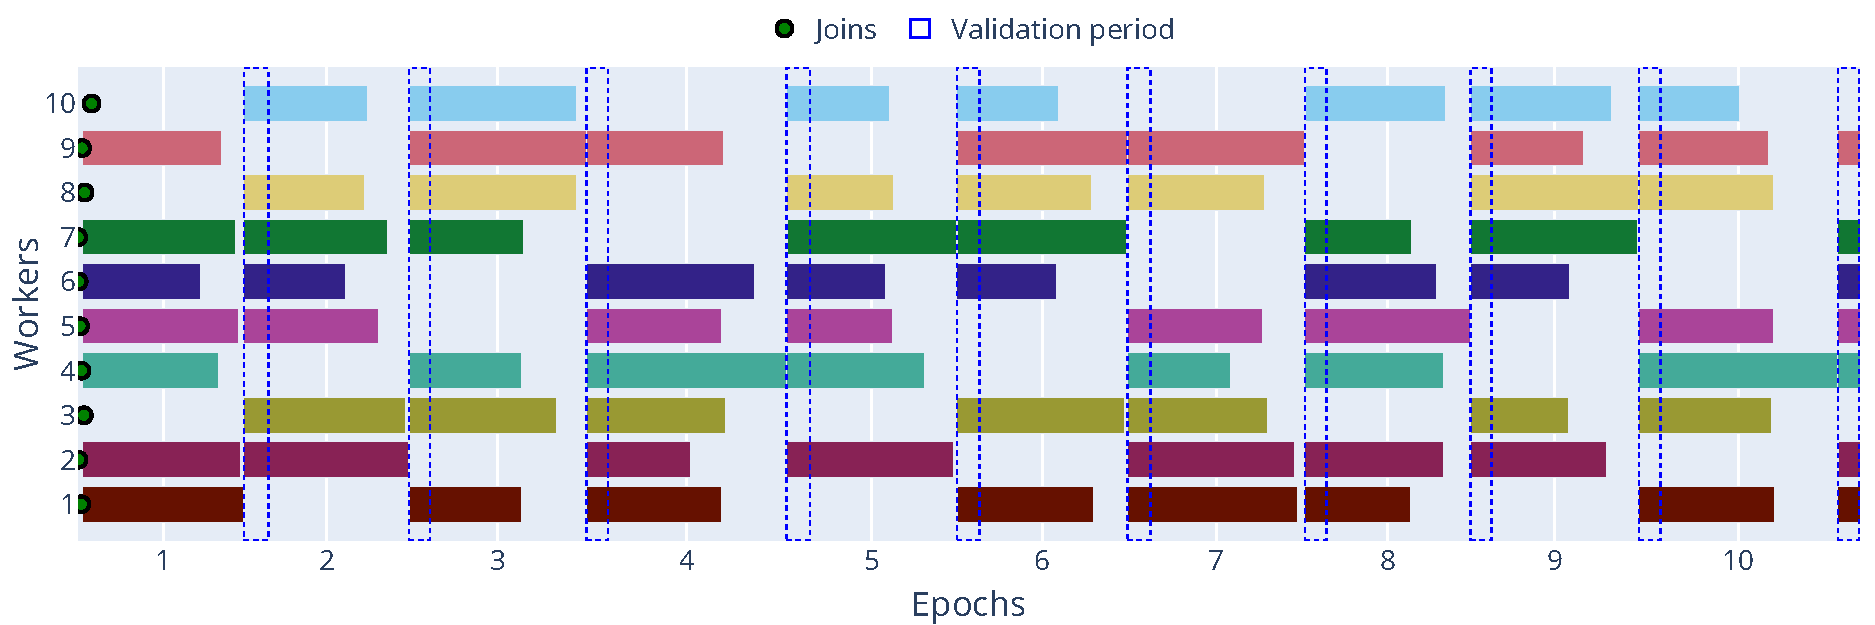
\includegraphics[width=\linewidth]{figs/scenario1/ds_timeline.pdf}
    \caption[Timeline of Decentralized Synchronous FL with Zenoh]{Timeline illustrating worker activity and idle periods across training epochs in the Decentralized Synchronous \ac{fl} approach with Zenoh, showing waiting for synchronization.}
    \label{fig:ds_timeline}
\end{figure}

\begin{figure}[!htb]
    \centering
    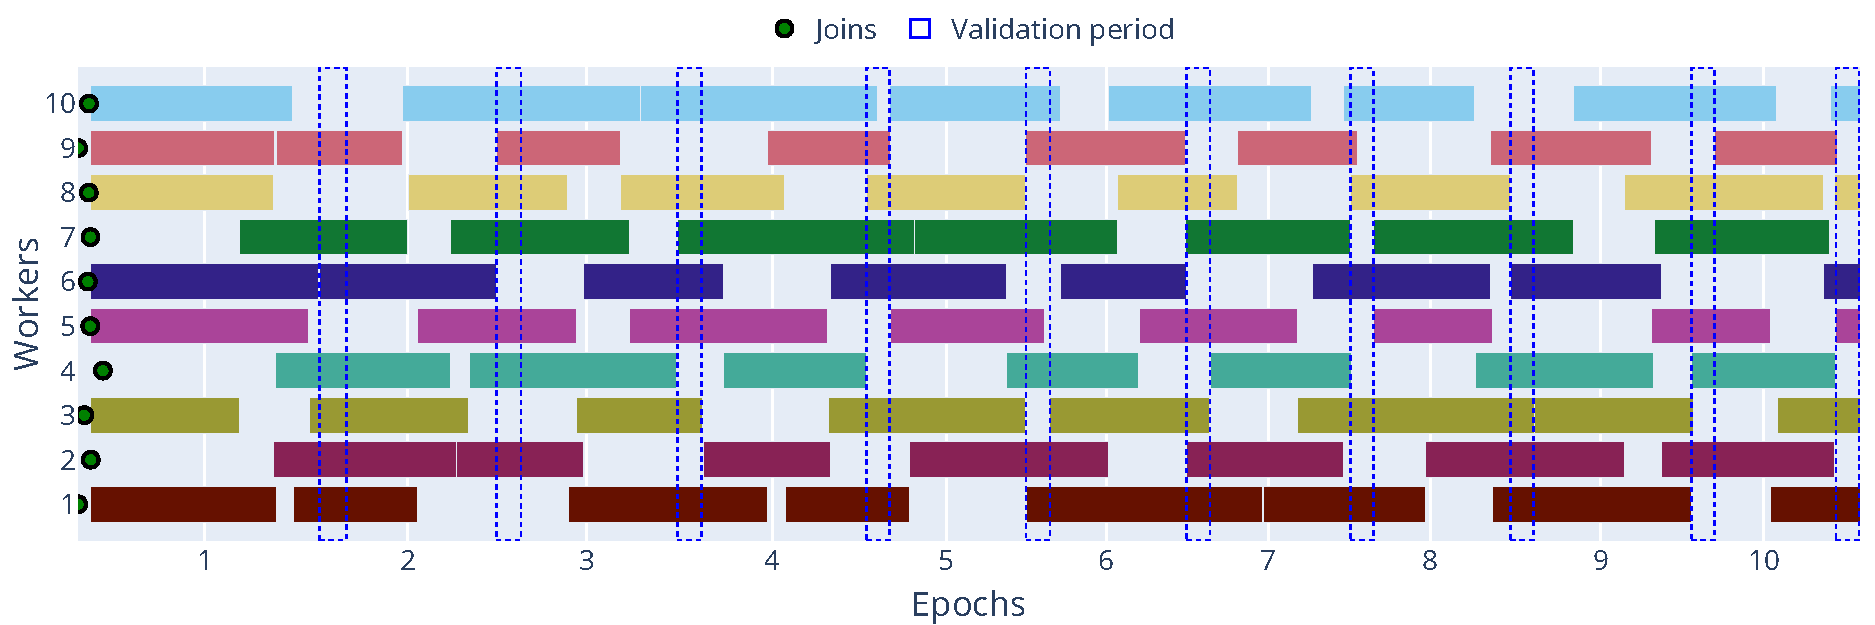
\includegraphics[width=\linewidth]{figs/scenario1/da_timeline.pdf}
    \caption[Timeline of Decentralized Asynchronous FL with Zenoh]{Timeline illustrating worker activity and idle periods across training epochs in the Decentralized Asynchronous \ac{fl} approach with Zenoh, demonstrating independent task completion and update submission.}
    \label{fig:da_timeline}
\end{figure}

This inherent advantage of asynchronous \ac{fl} is particularly critical in dynamic edge environments characterized by significant device heterogeneity, where worker speeds can vary drastically. When a worker joins, metadata is shared with the Parameter Server, this metadata can include information regarding their computational capabilities (e.g., CPU, memory, or GPU availability) and current network conditions (e.g., bandwidth and latency) and can be used in our modular Framework to implement more sophisticated scheduling policies to improve performance further. 

% Centralized has much more communication than Decentralized
As anticipated, Centralized methods involve a significantly higher frequency and volume of communication compared to Decentralized methods. For instance, across the Centralized experiments, the Parameter Server and workers exchanged a substantially larger number of messages (2285) and total payload size (403 MBs) compared to the Decentralized experiments, with 17 messages and a 2.7 MBs payload size.

% Centralized has much less local computation time than Decentralized - parameter server is doing the work and is a bottleneck 
We can also observe that workers in the Centralized approaches spend significantly less time on local computation compared to Decentralized workers. This discrepancy indicates that the server acts as a bottleneck in Centralized training, with workers spending considerable time idle or waiting for the server to aggregate updates and distribute the new global model, decreasing the local computation time from $\approx 83$ seconds in Decentralized approaches to $\approx 47$ seconds in Centralized approaches across all communication protocols.

% Centralized Asynchronous worse than Centralized Synchronous
This bottleneck effect was particularly noticeable in the Centralized Asynchronous setting, where the server must process every batch update from workers individually and immediately, potentially leading to increased server load and worker idle time, increasing the Total Run Time from 114 seconds in Decentralized Asynchronous with \ac{mqtt} to 744 seconds in the Centralized Asynchronous approach with the same communication protocol.

% Differences in payload size and number of messages
In asynchronous approaches, the number of messages exchanged and the total payload size vary from run to run, as reflected in standard deviations, due to the system dynamically adapting to worker availability. If a worker takes longer to complete their local training, other workers may complete more tasks, leading to a higher number of messages and a larger payload size. Conversely, in synchronous approaches, where workers proceed in lockstep, the number of messages and total payload size are expected to be the same across runs. 

This is the case for the Decentralized Synchronous approach, but not for the Centralized Synchronous approach. This is due to the number of iterations per epoch being determined by the total number of batches processed by the selected workers, if the dynamic worker pool selection results in different sets of workers (and thus potentially different total numbers of batches), it can introduce variability in the total number of iterations per round and consequently lead to varying numbers of messages and payload sizes.

\subsection{Communication Protocols Comparison}
\label{sec:communication-protocols-comparison}

% Overall overview of comm times
Observing the results in Table~\ref{tab:scenario_1_times}, distinct patterns emerge regarding the impact of the chosen communication protocol. Zenoh and \ac{mqtt} consistently exhibit lower average communication times across the tested \ac{fl} algorithm types compared to Kafka. Zenoh generally showed slightly lower communication times than \ac{mqtt}, although they were often closely comparable. 

\ac{mpi}, evaluated only in the Decentralized Synchronous context, showed higher communication times than Zenoh and \ac{mqtt} in that specific setting, and Kafka demonstrated the highest communication times across all paradigms where it was tested.

% Differences more evident in Centralized - more comm is done
This difference in communication performance is particularly evident when comparing the Centralized and Decentralized \ac{fl} approaches. Given the higher frequency and volume of communication, protocols with higher inherent latency, like Kafka, have a more pronounced negative impact on the overall communication time, achieving an average communication time of 360 seconds in the Centralized Synchronous compared to 23 and 25 seconds for Zenoh and \ac{mqtt}, respectively. 

% Similar working time - no comm overhead
In terms of average working time per worker, the communication protocol generally had a relatively similar impact across all protocols within the same \ac{fl} approach. This suggests that the time workers spend on local computation tasks is mainly independent of the communication method chosen, assuming the network does not become a severe bottleneck, completely halting progress. 

% parameter server comm in Sync approaches
Further analysis of Zenoh and \ac{mqtt} revealed that the average communication time was slightly higher in the Synchronous setting compared to the Asynchronous one. This observation suggests that the simultaneous arrival of synchronous updates from multiple workers at the central parameter server or broker might induce additional processing or queuing delays, which are then reflected in the increased communication time.

% Small std for times - stable runs, no significant outliers
Finally, analyzing the standard deviations across multiple runs provides valuable insights into the consistency and reliability of the framework's performance under different configurations. Low standard deviation values generally indicate that the experimental runs for a given configuration produced consistent results with no significant outliers, suggesting a stable and predictable behavior. 



\section{Scenario 2: Resilience Evaluation under Worker Failures}
\label{sec:scenario-2}


Building upon the foundational analysis of communication protocols and algorithms in Scenario 1, this scenario focuses specifically on evaluating the resilience mechanisms of the proposed Resilient Federated Learning Framework under simulated worker failures. The primary objective is to demonstrate the framework's ability to maintain training continuity and achieve model convergence even when individual worker nodes experience unexpected disconnections or failures.

The evaluation focused on the communication protocols best suited for dynamic and potentially unreliable network environments: Zenoh, \ac{mqtt}, and Kafka with the Decentralized Asynchronous \ac{fl} approach. This allows the training to proceed as long as there are active workers, processing updates as they arrive and naturally handling stragglers or failed nodes without waiting, by reassigning tasks and dynamically adapting to the available worker pool, which is crucial for resilience in dynamic environments.

To simulate worker failures, we introduced probabilistic failures into the system. Each worker was configured to have a certain probability of experiencing a failure event per second. We tested three different failure rates: 0.5\%, 1\%, and 3\% probability of failure per worker per second. 

When a failure occurred, the worker performed a graceful exit, simulating a planned shutdown or disengagement from the network, to ensure that logs are saved. Importantly, the framework was configured to allow failed workers to attempt to rejoin the training process shortly after the failure event, mimicking the behavior of real-world devices that might temporarily lose connectivity but eventually return.

To quantify the impact and handling of failures, we used the detailed system-level metrics, particularly focusing on the types of worker states described in Section~\ref{sec:metrics}:

\begin{itemize}
    \item \textbf{Non-critical failures:} These include \textit{iii: Failed while idle} and \textit{v: Failed after working successfully}. These failures are generally less disruptive as they do not interrupt an ongoing task that was assigned to the worker for the current round. The worker's contribution for the round, if any, was already submitted, or no task was missed.
    \item \textbf{Critical failures:} This refers to the \textit{iv: Failed while working} state, where a worker fails while actively performing its assigned task (local computation or communication). This type of failure is more disruptive as the partial or completed work for that task is lost, potentially requiring rescheduling or impacting the aggregation process, depending on the algorithm and framework's handling mechanisms.
\end{itemize}

Additionally, the other two states, \textit{i: Idle without fail} and \textit{ii: Worked successfully without failing}, are not directly related to failures but provide context for the worker's activity during the training process.

Table~\ref{tab:scenario-2-failures} presents a summary of the observed failure counts across the evaluated communication protocols and failure rates in the Decentralized Asynchronous setting.

\begin{table}[!htb]
    \centering
    \caption[Worker Failures in Decentralized Asynchronous FL]{Summary of observed worker failures during training with the Decentralized Asynchronous approach, detailing counts of non-critical, critical, and total failures, alongside the total run duration for each communication protocol and failure rate.}
    \label{tab:scenario-2-failures}
    \begin{tabular}{Sc Sc Sc Sc Sc Sc}
        \toprule
        \textbf{Failure Rate} &
        \textbf{\begin{tabular}[c]{@{}c@{}}Comm\\Protocol\end{tabular}} &
        \textbf{\begin{tabular}[c]{@{}c@{}}Non-Critical\\Failures\end{tabular}} &
        \textbf{\begin{tabular}[c]{@{}c@{}}Critical\\Failures\end{tabular}} &
        \textbf{\begin{tabular}[c]{@{}c@{}}Total\\Failures\end{tabular}} &
        \textbf{\begin{tabular}[c]{@{}c@{}}Total Run\\Duration (s)\end{tabular}} \\
        \midrule
        \multirow{3.5}{*}{\begin{tabular}[c]{@{}c@{}}0.5\% every\\Second\end{tabular}}
        & Zenoh & 3 & 5 & 8 & 123.3 \\
        & MQTT  & 2 & 6 & 8 & 125.0 \\
        & Kafka & 1 & 7 & 8 & 121.6 \\
        \midrule
        \multirow{3.5}{*}{\begin{tabular}[c]{@{}c@{}}1\% every\\Second\end{tabular}}
        & Zenoh & 3 & 10 & 13 & 123.8 \\
        & MQTT  & 2 & 12 & 14 & 129.5 \\
        & Kafka & 5 & 8  & 13 & 124.1 \\
        \midrule
        \multirow{3.5}{*}{\begin{tabular}[c]{@{}c@{}}3\% every\\Second\end{tabular}}
        & Zenoh & 8 & 30 & 38 & 149.4 \\
        & MQTT  & 2 & 38 & 40 & 155.7 \\
        & Kafka & 7 & 37 & 44 & 170.6 \\
        \bottomrule
    \end{tabular}
\end{table}

% All runs completed successfully
The results from this scenario provide strong empirical evidence for the framework's resilience. A key observation is that all experimental runs, regardless of the communication protocol or failure rate, completed successfully. This demonstrates that the framework's built-in mechanisms, such as the dynamic worker pool, task rescheduling for asynchronous approaches, and the Parameter Server's ability to handle sporadic updates, are effective in allowing the training process to continue and converge despite the presence of worker failures.

% Total number of failures increased with failure rate
As expected, the total number of observed failures increased significantly as the probabilistic failure rate was increased from 0.5\% to 3\%. While the runs for each configuration were initiated with the same random seed to promote consistency, slight variations in the exact number of failures occurred across different runs. 

% why same seed different values
This variability is inherent in the dynamic nature of the simulation, where factors such as the precise timing of failure events, the varying working times of individual workers, and the dynamic selection of workers for the subpool in each round can influence which workers are active and thus susceptible to failure at any given moment. 

% exaggerated failure rates as stress test
It is worth noting that a 1\% and 3\% failure rate per second represents an extremely chaotic and likely unrealistic scenario for most real-world deployments, serving as a stress test for the framework's robustness.

% higher run times - rescheduling
As anticipated, introducing failures led to a modest increase in the average total run time compared to the no-failure baseline. For the 0.5\% and 1\% failure rates, the increase was relatively small, varying with the training progress that needs to be rescheduled due to Critical Failures. 

% higher run times - pause training
However, at the 3\% failure rate, the increase in run time was more pronounced, this greater increase can be attributed not only to the higher volume of critical failures and subsequent task rescheduling but also to periods where the training process might have paused. The framework is designed to ensure a minimum number of active workers are available in each round to maintain training, if the dynamic worker pool drops below this threshold (7 workers or 70\% of the 10 workers), the parameter server pauses the training, by not sending new tasks and waits for enough workers to become available to proceed.

% visualizing results
To provide a deeper understanding of how failures were handled and their impact on the training process, we visualize the results through timelines, worker state matrices, and validation loss curves. Figure~\ref{fig:results_kafka}, Figure~\ref{fig:results_mqtt}, and Figure~\ref{fig:results_zenoh} illustrate the results for the Kafka, \ac{mqtt}, and Zenoh protocols, for the 0.5\%, 1\%, and 3\% failure rates, respectively. These visualizations offer a comprehensive overview of the behavior of various communication protocols under different failure scenarios.

\begin{figure}[!htb]
    \centering
    \begin{subfigure}[b]{\linewidth}
        \centering
        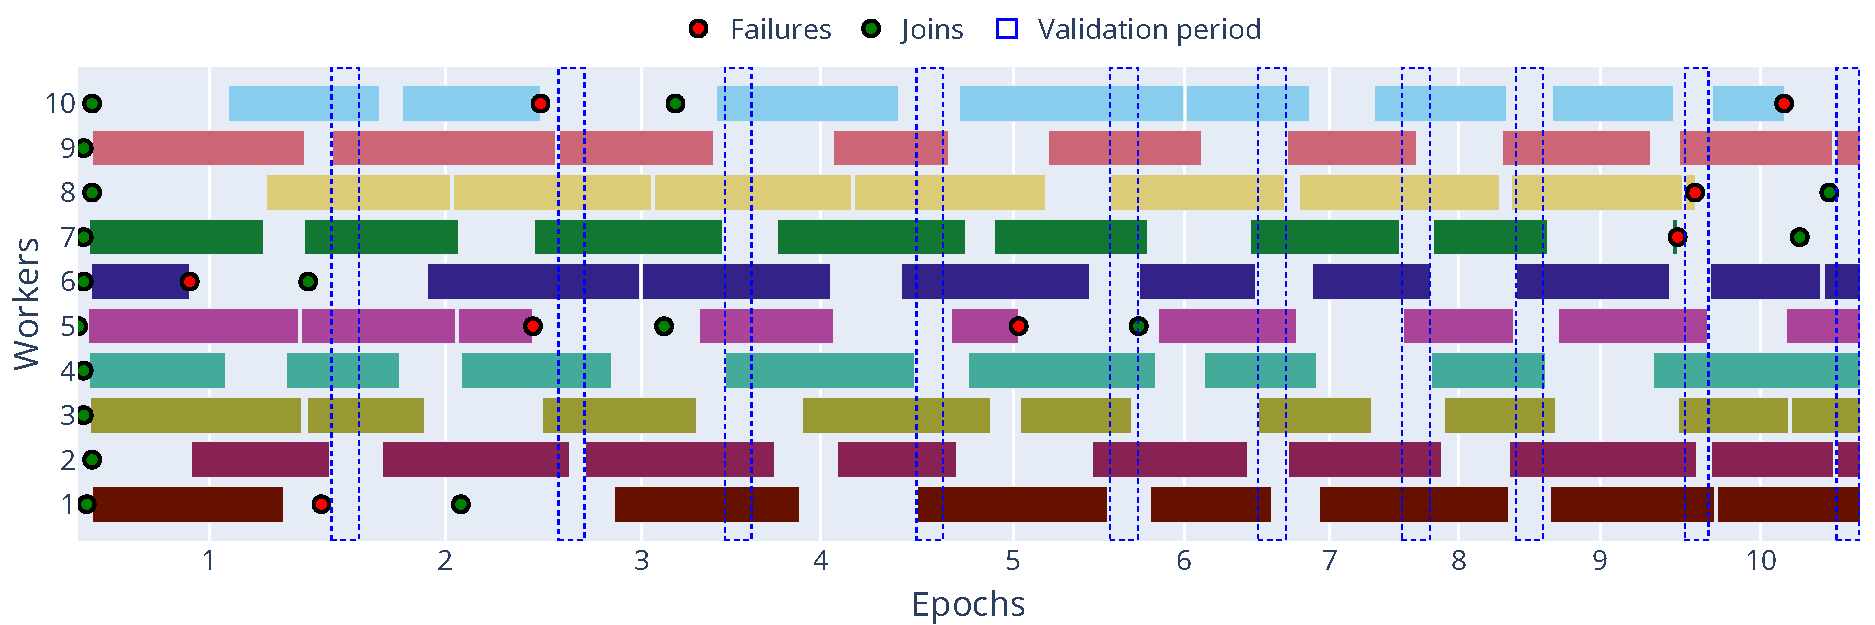
\includegraphics[width=\linewidth]{figs/scenario2/kafka_timeline.pdf}
        \caption{Timeline of worker activity and failure events.}
        \label{fig:timeline_kafka}
    \end{subfigure}
    \begin{subfigure}[b]{0.6\linewidth}
        \centering
        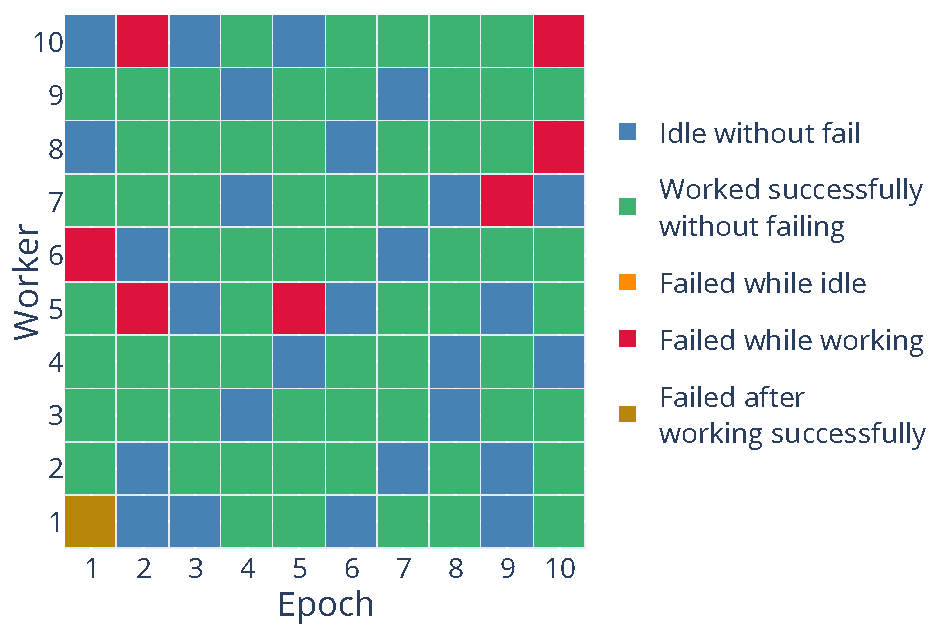
\includegraphics[width=\linewidth]{figs/scenario2/kafka_status.pdf}
        \caption{Worker state matrix across training epochs.}
        \label{fig:states_kafka}
    \end{subfigure}
    % \hfill
    \begin{subfigure}[b]{0.6\linewidth}
        \centering
        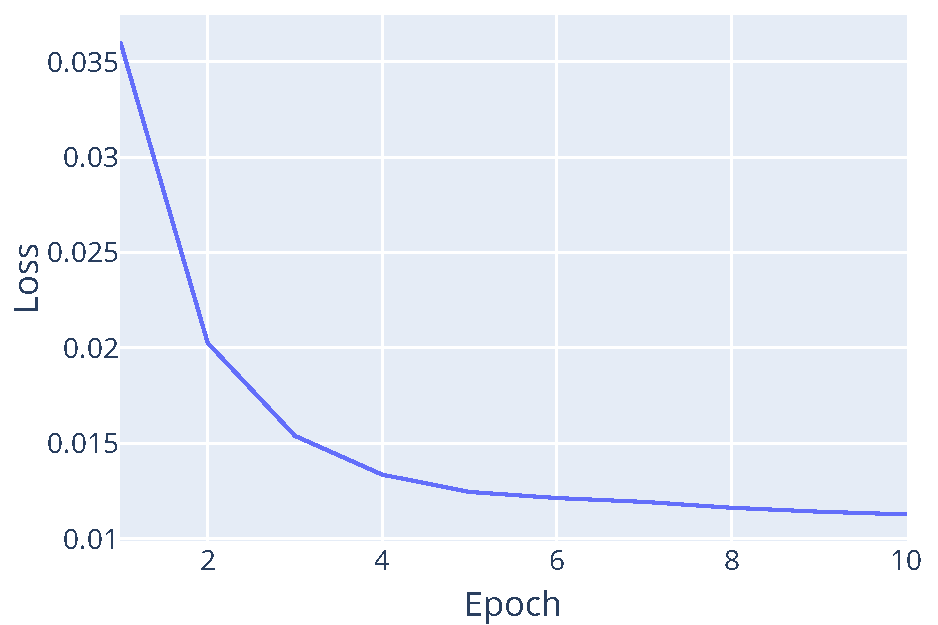
\includegraphics[width=\linewidth]{figs/scenario2/kafka_loss.pdf}
        \caption{Validation loss curve.}
        \label{fig:loss_kafka}
    \end{subfigure}
    \caption{Training results with the Kafka protocol (0.5\% failure rate).}
    \label{fig:results_kafka}
\end{figure}

\begin{figure}[!htb]
    \centering
    \begin{subfigure}[b]{\linewidth}
        \centering
        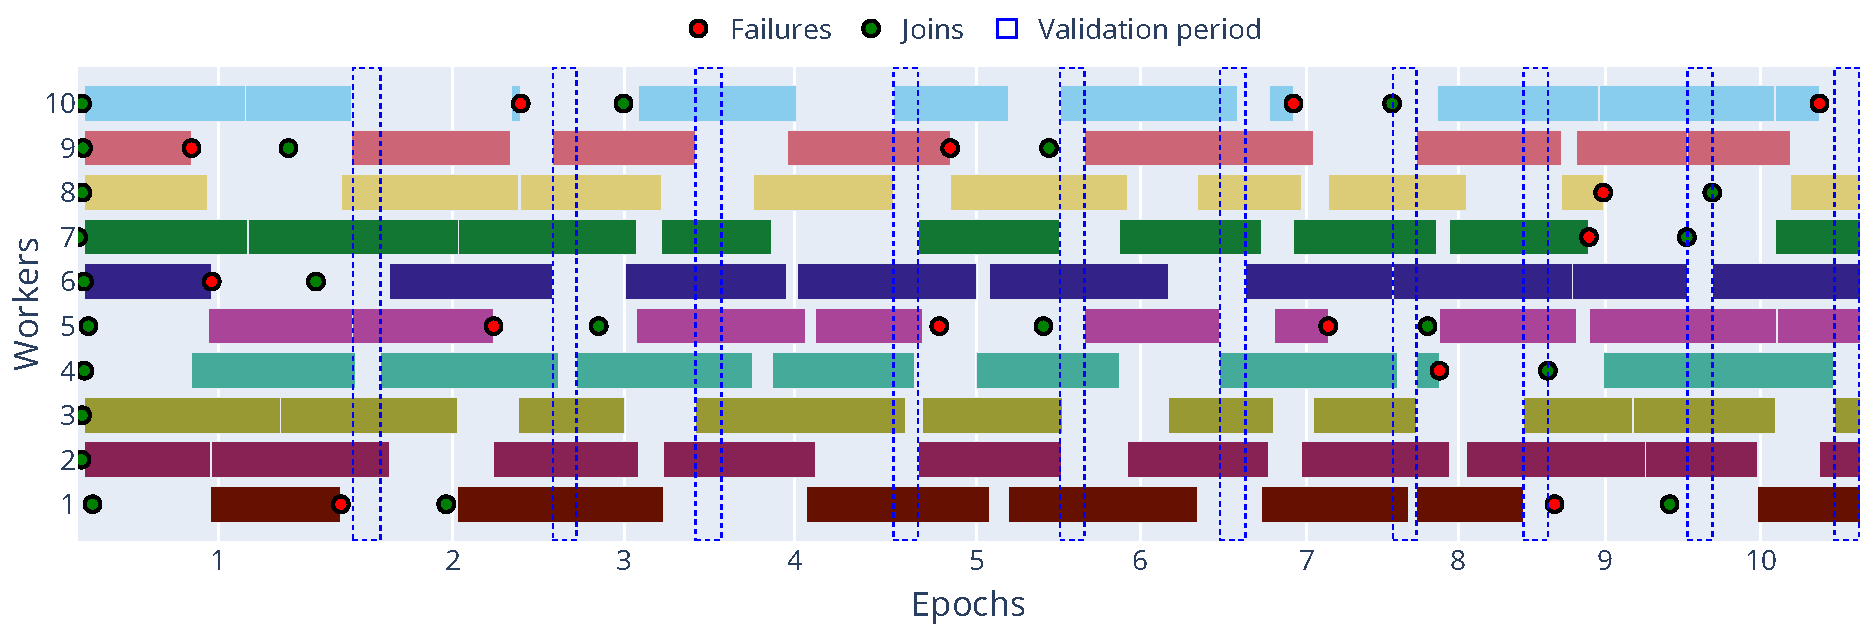
\includegraphics[width=\linewidth]{figs/scenario2/mqtt_timeline.pdf}
        \caption{Timeline of worker activity and failure events.}
        \label{fig:timeline_mqtt}
    \end{subfigure}
    \begin{subfigure}[b]{0.6\linewidth}
        \centering
        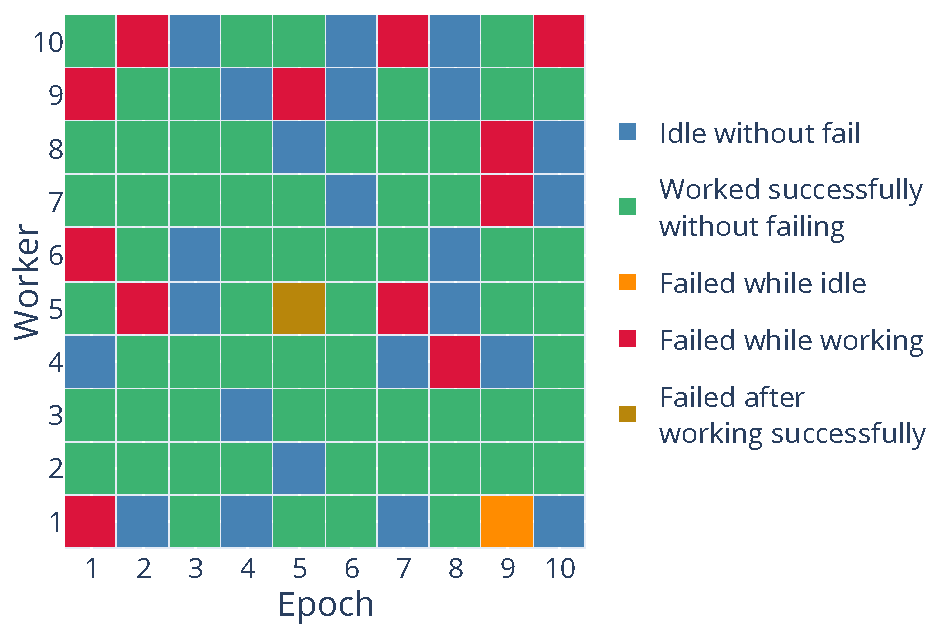
\includegraphics[width=\linewidth]{figs/scenario2/mqtt_status.pdf}
        \caption{Worker state matrix across training epochs.}
        \label{fig:states_mqtt}
    \end{subfigure}
    % \hfill
    \begin{subfigure}[b]{0.6\linewidth}
        \centering
        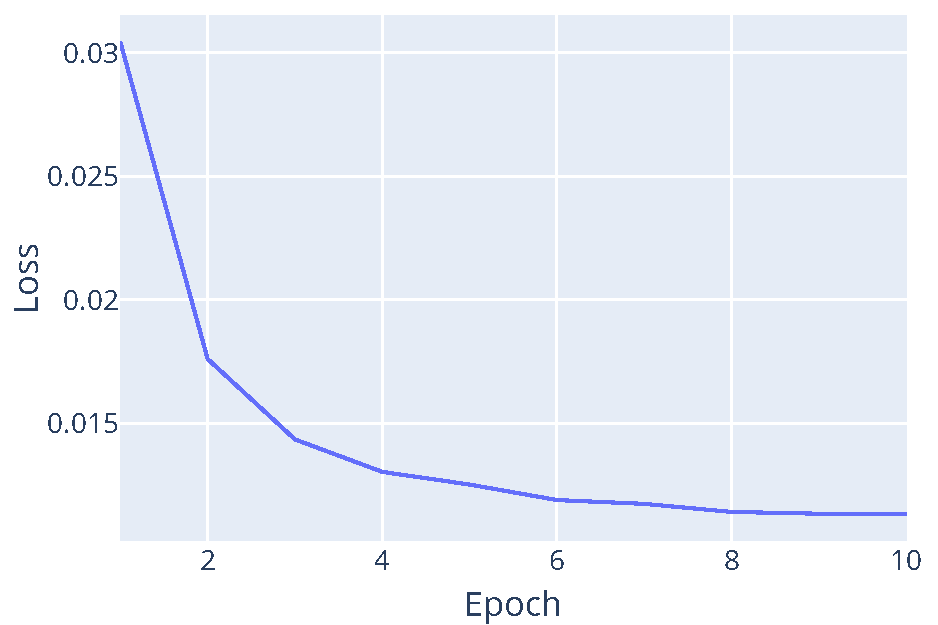
\includegraphics[width=\linewidth]{figs/scenario2/mqtt_loss.pdf}
        \caption{Validation loss curve.}
        \label{fig:loss_mqtt}
    \end{subfigure}
    \caption[]{Training results with the MQTT protocol (1\% failure rate).}
    \label{fig:results_mqtt}
\end{figure}

\begin{figure}[!htb]
    \centering
    \begin{subfigure}[b]{\linewidth}
        \centering
        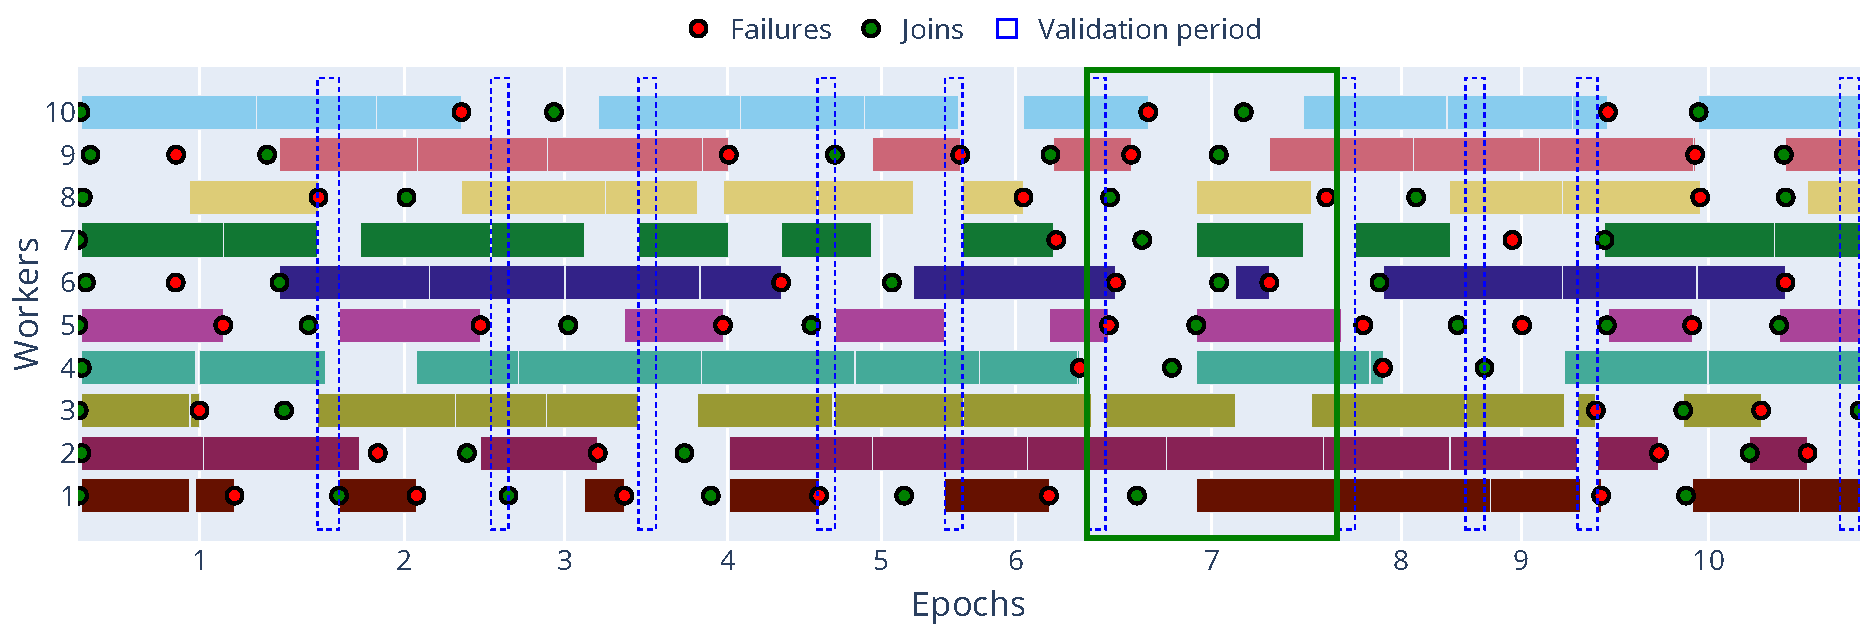
\includegraphics[width=\linewidth]{figs/scenario2/zenoh_timeline.pdf}
        \caption{Timeline of worker activity and failure events.}
        \label{fig:timeline_zenoh}
    \end{subfigure}
    \begin{subfigure}[b]{0.6\linewidth}
        \centering
        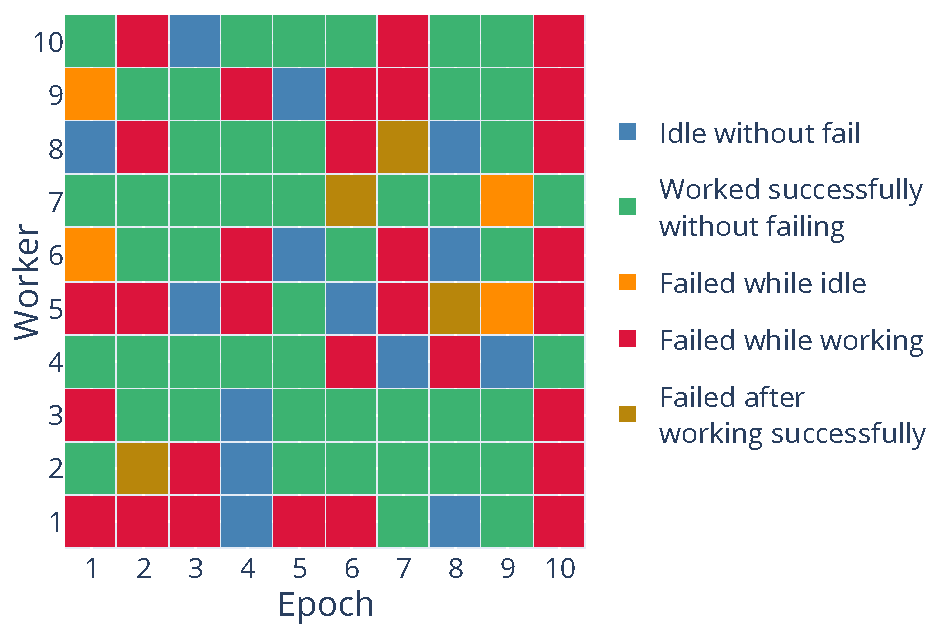
\includegraphics[width=\linewidth]{figs/scenario2/zenoh_status.pdf}
        \caption{Worker state matrix across training epochs.}
        \label{fig:states_zenoh}
    \end{subfigure}
    % \hfill
    \begin{subfigure}[b]{0.6\linewidth}
        \centering
        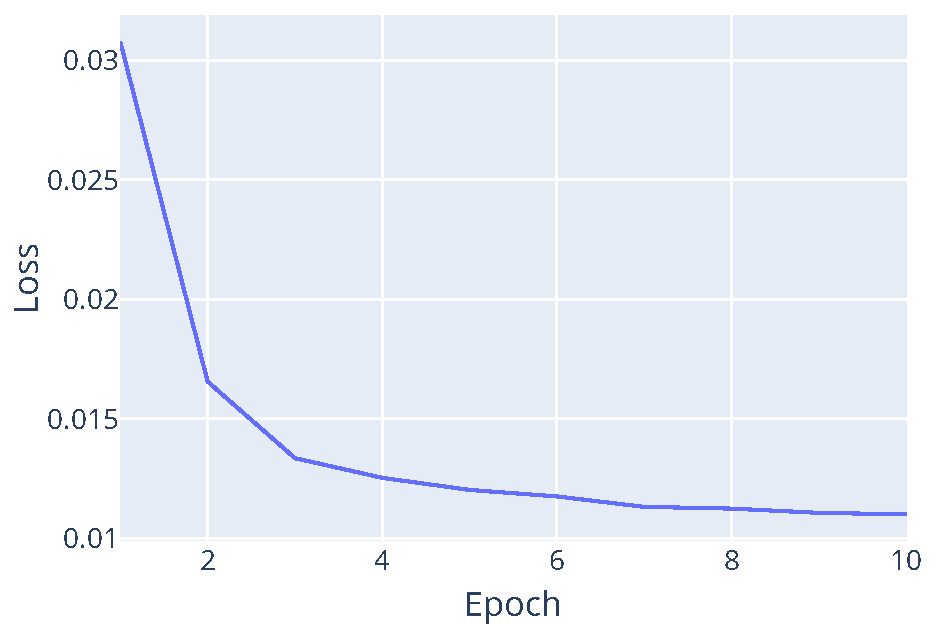
\includegraphics[width=\linewidth]{figs/scenario2/zenoh_loss.pdf}
        \caption{Validation loss curve.}
        \label{fig:loss_zenoh}
    \end{subfigure}
    \caption{Training results with the Zenoh protocol (3\% failure rate).}
    \label{fig:results_zenoh}
\end{figure}

% timelines and rescheduling 
We can observe that the timelines show the activity (working, idle) of each worker over time, clearly marking when failure events occurred and when workers rejoined the network. They also illustrate how the Parameter Server reacted to critical failures, such as rescheduling tasks in the Decentralized Asynchronous setting. Specifically, when a worker fails while working or finishes their task, the Parameter Server sends a new task to another worker as soon as possible, allowing the training to continue without significant delays.

% pause training
In cases where the number of active workers dropped below the threshold (7 workers), the Parameter Server paused the training until enough workers were available to proceed. This is evident in Figure~\ref{fig:timeline_zenoh} at epoch 7, as soon as the number of workers reached the threshold (when worker 5 joined), the parameter server resumed the training process by sending new tasks to 5 workers $\{1, 4, 5, 7, 8\}$, while 2 were already working on their tasks $\{2, 3\}$ and the remaining 3 workers were offline due to failures $\{6, 9, 10\}$.

% worker state matrices
The worker state matrices offer a clear, epoch-by-epoch view of each worker's state (Idle without fail, Worked successfully, Failed while idle, Failed while working, Failed after working successfully), making it easier to evaluate the frequency and type of failures experienced by individual workers throughout the experiment. 

% loss plots
Finally, plots showing the validation loss curve over epochs for representative runs (Kafka with 0.5\% failure rate, MQTT with 1\% failure rate, and Zenoh with 3\% failure rate) visually confirm that the model consistently converged, even under the highest simulated failure rate, demonstrating that the framework's resilience mechanisms effectively preserved the integrity of the training process and allowed the model to learn despite the disruptions.



\section{Scenario 3: Scalability and Convergence with Large-Scale Failures}
\label{sec:scenario-3}

This final scenario is designed to push the boundaries of the Resilient Federated Learning Framework by evaluating its scalability and overall robustness when operating with a significantly larger worker pool and simultaneously introducing substantial simulated failures. The objective is to demonstrate that the framework can effectively scale the training process and achieve model convergence even in a large-scale, dynamic \ac{fl} environment where numerous worker nodes are experiencing disruptions.

For this evaluation, we used the combined worker set, comprising both the uniform set (10 \acp{vm}) and the heterogeneous set (30 \acp{vm}), totaling 40 worker \acp{vm}. This configuration provides a more realistic representation of real-world \ac{fl} deployments, involving a diverse group of devices with varying computational capabilities and network conditions.

Given the significantly larger worker pool (40 \acp{vm} compared to 10 in previous scenarios), the total dataset was partitioned across a greater number of devices. Consequently, each worker had access to a smaller local data subset. To ensure robust model convergence and to adequately compensate for the reduced training data available per client in each round, the number of training epochs was increased from 10 to 20. This adjustment enables more global aggregation steps, which is crucial for achieving comparable model quality and convergence in environments with distributed and sparse data partitions.

Based on the findings from Scenario 1 and Scenario 2, we selected the Decentralized Asynchronous algorithm due to its inherent suitability for dynamic environments and resilience to failures, and the Zenoh communication protocol, which consistently exhibited lower communication overhead and native support for dynamic participant management. This combination is expected to be the most robust for large-scale, failure-prone scenarios.

The experiments in this scenario were conducted using both the UNSW-NB15 and ToN-IoT datasets. Evaluating the framework with two distinct datasets demonstrates its versatility and ability to handle different data characteristics and problem domains at scale. Both datasets were configured for the binary classification task, as described in Section~\ref{sec:datasets-and-models}, with data partitioned using the \ac{iid} strategy.

Simulated worker failures were introduced at a 1\% probabilistic failure rate per worker per second. This rate represents a significant level of churn and disruption across the 40 worker nodes, testing the framework's ability to maintain continuity under considerable stress.

Table~\ref{tab:scenario-3-failures} presents the average counts of non-critical, critical, and total failures observed across runs for each dataset at the 1\% failure rate.

\begin{table}[!htb]
    \centering
    \caption[Worker Failures and Run Time at 1\% Rate with 40 Workers]{Failure counts observed during training with the Decentralized Asynchronous approach and a 1\% failure rate with 40 workers, detailing non-critical, critical, and total failures, alongside the total run duration for both the UNSW-NB15 and ToN-IoT datasets.}
    \label{tab:scenario-3-failures}
    \begin{tabular}{Sc Sc Sc Sc Sc}
        \toprule
        \textbf{Dataset} &
        \textbf{\begin{tabular}[c]{@{}c@{}}Non-Critical\\Failures\end{tabular}} &
        \textbf{\begin{tabular}[c]{@{}c@{}}Critical\\Failures\end{tabular}} &
        \textbf{\begin{tabular}[c]{@{}c@{}}Total\\Failures\end{tabular}} &
        \textbf{\begin{tabular}[c]{@{}c@{}}Total Run\\Duration (s)\end{tabular}} \\
        \midrule
        UNSW-NB15 & 9 & 8 & 17 & 62.6 \\
        ToN-IoT & 20 & 27 & 47 & 122.5 \\
        \bottomrule
    \end{tabular}
\end{table}

% runs completed successfully
Similar to Scenario 2, all experimental runs in this scenario, for both datasets and with the 40-worker setup and 1\% failure rate, completed successfully. This further validates the framework's resilience mechanisms, which effectively managed the dynamic worker pool and allowed for continuous training despite the presence of numerous worker failures. This is a critical finding, demonstrating that the framework scales effectively and maintains its resilience properties even under increased load and disruption.

% run times - unsw comparison
Comparing the total run durations, for the UNSW-NB15 dataset, the total run duration of 62 seconds compared to 123 seconds in Scenario 2 with 10 workers and the same failure rate, this counter-intuitive result, despite the increased number of epochs (20 vs. 10), is primarily due to the data partitioning strategy. With 40 workers instead of 10, each worker processed approximately one-quarter of the total training data per local epoch. While the total number of global epochs doubled, the reduced local training time per worker per epoch, combined with the asynchronous nature of the algorithm, allowed for continuous progress without waiting for all stragglers, enabling a faster overall completion due to increased parallelization.

% run times - toniot
Conversely, the ToN-IoT dataset resulted in a significantly longer average total run duration of 122.5 seconds compared to UNSW-NB15 (62.6 seconds) in this scenario. As noted in Section~\ref{sec:datasets-and-models}, the ToN-IoT dataset is considerably larger than UNSW-NB15 (over 13 million samples versus 2 million), and despite the ToN-IoT model having a smaller architecture, the sheer volume of data in ToN-IoT requires more extensive local computation per worker, leading to a longer overall training duration.

To visually illustrate the training process at scale, Figures~\ref{fig:scenario3_unsw_results} and \ref{fig:scenario3_toniot_results} show the validation loss and other key epoch metrics over training epochs for a representative run for the UNSW-NB15 and ToN-IoT datasets, respectively.

\begin{figure}[!htb]
    \centering
    \begin{subfigure}[b]{0.49\linewidth}
        \centering
        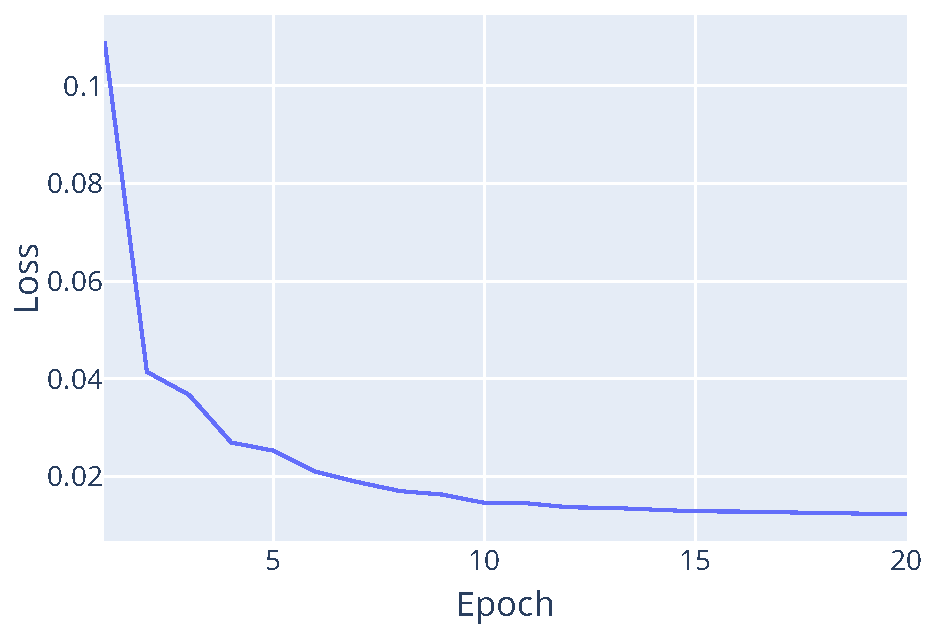
\includegraphics[width=\linewidth]{figs/scenario3/unsw_loss.pdf}
        \caption{Validation loss curve for UNSW-NB15 dataset.}
        \label{fig:scenario3_unsw_loss}
    \end{subfigure}
    \hfill
    \begin{subfigure}[b]{0.49\linewidth}
        \centering
        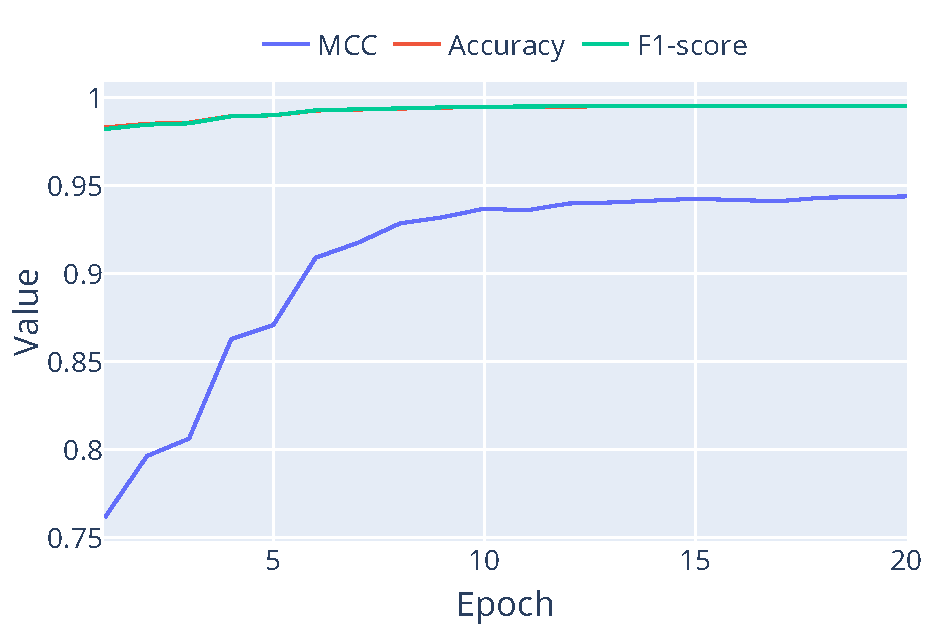
\includegraphics[width=\linewidth]{figs/scenario3/unsw_metrics.pdf}
        \caption{Epoch metrics for UNSW-NB15 dataset.}
        \label{fig:scenario3_unsw_metrics}
    \end{subfigure}
    \caption[UNSW-NB15 Training Results with Decentralized Asynchronous FL]{Training results with the UNSW-NB15 dataset using Decentralized Asynchronous approach and Zenoh protocol with 40 workers and 1\% failure rate.}
    \label{fig:scenario3_unsw_results}
\end{figure}

\begin{figure}[!htb]
    \centering
    \begin{subfigure}[b]{0.49\linewidth}
        \centering
        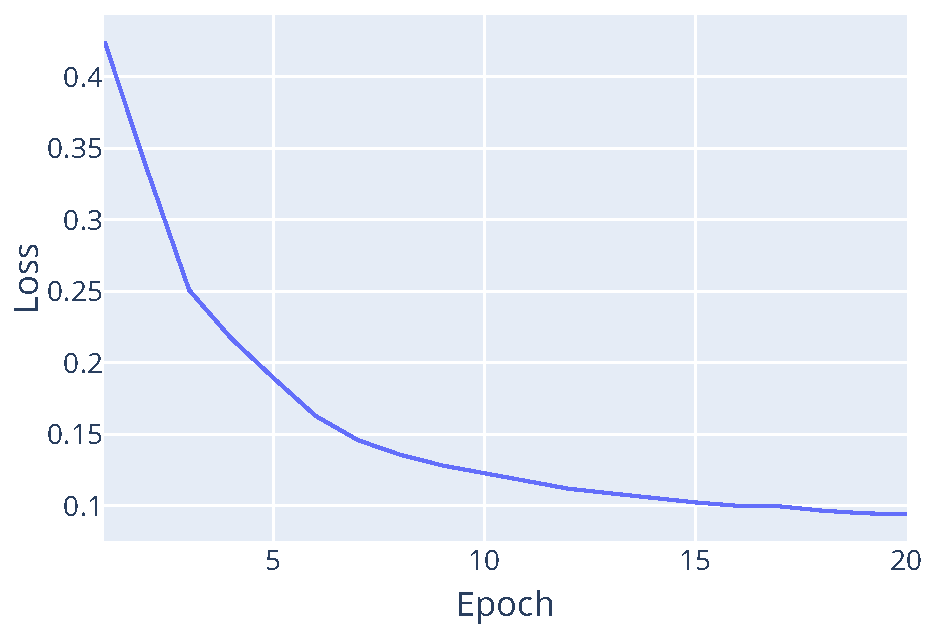
\includegraphics[width=\linewidth]{figs/scenario3/toniot_loss.pdf}
        \caption{Validation loss curve for ToN-IoT dataset.}
        \label{fig:scenario3_toniot_loss}
    \end{subfigure}
    \hfill
    \begin{subfigure}[b]{0.49\linewidth}
        \centering
        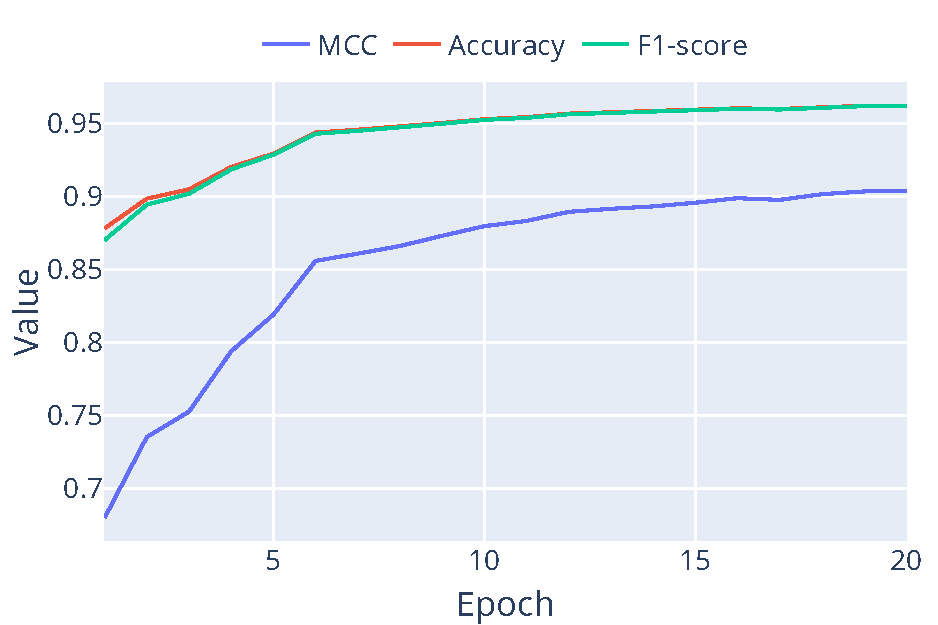
\includegraphics[width=\linewidth]{figs/scenario3/toniot_metrics.pdf}
        \caption{Epoch metrics for ToN-IoT dataset.}
        \label{fig:scenario3_toniot_metrics}
    \end{subfigure}
    \caption[ToN-IoT Training Results with Decentralized Asynchronous FL]{Training results with the ToN-IoT dataset using Decentralized Asynchronous approach and Zenoh protocol with 40 workers and 1\% failure rate.}
    \label{fig:scenario3_toniot_results}
\end{figure}

These plots provide visual confirmation of the framework's ability to maintain stable training and achieve model convergence even under the demanding conditions of Scenario 3, characterized by a large and heterogeneous worker pool and frequent simulated failures. 

For both datasets, the validation loss curves consistently decrease over epochs, indicating that the models are effectively learning and improving. Simultaneously, the MCC, Accuracy, and F1-score metrics exhibit a clear upward trend, converging towards high-performance values, which demonstrates the framework's robustness in ensuring model quality despite disruptions.

The successful completion of all runs in this challenging scenario, coupled with clear evidence of model convergence and high final performance metrics, validates the core design principles of the Resilient Federated Learning Framework. It proves its capability to effectively manage dynamic worker participation, tolerate significant node failures, and adapt to varying data and network conditions. 

For the UNSW-NB15 dataset, the final MCC achieved was 0.944, and for the ToN-IoT dataset, it was 0.903, further underlining the effectiveness of the training process even under adverse conditions. This comprehensive evaluation demonstrates that the framework is a robust and scalable solution for real-world Federated Learning deployments, particularly in edge computing environments where resilience and efficiency are paramount.

\chapter{Conclusion}
\label{chap:conclusion}

\begin{introduction}

This chapter summarizes the key contributions of the Resilient Federated Learning Framework, discusses its limitations, and proposes directions for future research, reinforcing its role in advancing robust and scalable FL deployments.


\end{introduction}

\section{Findings and Accomplishments}

The growing prevalence of \ac{ai} applications in dynamic, resource-constrained edge environments, significantly enabled by technologies like 5G/6G and the proliferation of \ac{iot} devices, underscores the critical need for robust and scalable distributed \ac{ml} paradigms such as \ac{fl}.

However, deploying \ac{fl} effectively in these real-world settings presents considerable technical challenges, particularly concerning fault tolerance, elasticity to dynamic participation, and communication efficiency under variable network conditions. This dissertation addressed these key issues by proposing, implementing, and evaluating a novel \ac{fl} framework explicitly designed for resilience and modularity. Guided by the challenges, this research specifically aimed to answer:

\begin{itemize}
    \item \textbf{RQ1:} How can Federated Learning frameworks be designed to ensure robustness against node failures across dynamic network environments?
    \item \textbf{RQ2:} What communication layer architectures are most suitable for supporting fault-tolerant and resilient Federated Learning under dynamic network conditions?
\end{itemize}

The core of our proposed framework is its highly modular architecture, comprising seven decoupled components responsible for distinct aspects of the \ac{fl} process, including communication layer, \ac{fl} algorithms, and worker management. This design shows remarkable flexibility, allowing for straightforward integration and experimentation with various \ac{ml} libraries, communication protocols, and \ac{fl} strategies without requiring extensive modifications to the entire system. 

This modularity directly contributes to the framework's adaptability, enabling it to be tailored to diverse requirements and constraints encountered in different edge computing scenarios, and crucially, facilitates the integration of features that enhance resilience.

In response to the first research question regarding how to design \ac{fl} frameworks for robustness against node failures in dynamic environments, our work focused on implementing key mechanisms within the framework's architecture. These include a dynamic worker pool managed by the Worker Manager module to handle device joins and leaves seamlessly, configurable completion thresholds for synchronous \ac{fl} approaches to tolerate stragglers without halting progress, and task rescheduling mechanisms for asynchronous \ac{fl} to ensure that tasks from failed workers are reassigned and completed.

The empirical evaluation in Scenario 2 and Scenario 3 (Sections \ref{sec:scenario-2} and \ref{sec:scenario-3}), simulating significant probabilistic worker failures across various configurations, demonstrated that the framework successfully maintained training continuity and model convergence, evidenced by the high final MCC values of 0.944 for the UNSW-NB15 dataset and 0.903 for the ToN-IoT dataset with 40 workers and 1\% failure rate every second, providing strong evidence that these specific design choices effectively contribute to resilience under dynamic and adverse conditions.

Addressing the second research question concerning what communication layer architectures are most suitable for fault-tolerant and resilient \ac{fl} under dynamic network conditions, the evaluation conducted in Scenario 1 (Section \ref{sec:scenario-1}) provided critical comparative insights into communication efficiency and overhead. By testing Zenoh, \ac{mqtt}, and Kafka, we observed that protocol characteristics identified in this scenario significantly influence overall system performance and, crucially, robustness in the failure scenarios investigated in other experiments.

Protocols with native support for dynamic participant management and efficient handling of sporadic messages, such as Zenoh and \ac{mqtt}, generally exhibited better suitability for dynamic, failure-prone environments. Their built-in disconnection detection mechanisms proved advantageous compared to protocols like Kafka, which required additional application-level heartbeats in our implementation. 

Zenoh's decentralized nature further enhances its potential resilience by avoiding a single point of failure associated with a centralized broker. This comparative analysis highlights that the suitability of communication protocols is indeed variable, with Zenoh and \ac{mqtt} demonstrating stronger alignment with the requirements for resilient \ac{fl} in dynamic edge settings based on our empirical findings.

In summary, this research contributes with a modular and Resilient Federated Learning Framework, validated through experimental evaluation, that effectively addresses critical challenges in dynamic edge environments. The framework's design and implementation, coupled with the insights gained from the experimental scenarios regarding both the mechanisms for ensuring robustness and the comparative suitability of communication protocols, provide a strong foundation for developing more robust and adaptable \ac{fl} systems for real-world applications where data privacy, security, and continuous operation are paramount.



\section{Limitations}
\label{sec:limitations}

While the proposed framework demonstrates promising capabilities, it is important to acknowledge certain limitations inherent in the current study and experimental setup. The evaluation was primarily conducted in a controlled, simulated environment using \acp{vm}, although this setup allowed for systematic testing under configurable conditions, it does not fully replicate the complexity and variability of real-world deployments.

Specifically, the worker nodes were implemented as \acp{vm} with relatively similar hardware specifications (CPU, memory). Real-world edge devices exhibit significant heterogeneity in computational capabilities, which can significantly impact \ac{fl} performance and convergence. 

Furthermore, the evaluation primarily focused on approximating \ac{iid} data distribution across workers. Real-world \ac{fl} scenarios frequently involve highly divergent, \ac{non-iid} data distributions, which pose additional challenges for model convergence and fairness that were not exhaustively explored in this evaluation. 

The simulated worker failures predominantly involved graceful exits followed by potential re-joins, which may not fully capture the unpredictable nature and impact of abrupt crashes, sudden power losses, or prolonged network disconnections often encountered in practice. 

Finally, while the framework is designed for scalability, the experimental validation involved a relatively small number of worker \acp{vm} (10 in the uniform set, 40 in the heterogeneous set), which provides valuable insights but does not definitively validate its performance and scalability to massive \ac{fl} deployments involving potentially hundreds of devices.



\section{Future Work}
\label{sec:future-work}


Building upon the foundation established by this research, several promising avenues for future work can be pursued to enhance the framework and broaden its evaluation. A primary direction is to expand the experimental validation to more closely approximate challenging real-world scenarios. 

Crucially, future work should involve rigorous testing under \ac{non-iid} data distributions to assess the framework's performance and explore strategies for mitigating the associated convergence and fairness challenges. The framework's modular design, particularly the \ac{fl} Backend, offers a key advantage here by enabling integration of advanced aggregation strategies and intelligent client selection mechanisms that prioritize data diversity or balance contributions from heterogeneous data distributions \cite{zhao2018federated}. 

Furthermore, the Dataset Manager module could incorporate local data augmentation, re-sampling techniques, or privacy-preserving methods to expose local data statistics that the \ac{fl} Backend could use for more informed aggregation and an improved scheduling policy. Evaluating the framework with other types of datasets beyond \ac{ids}/\ac{iot}, such as those from healthcare or finance, would also demonstrate its versatility.

Investigating the trade-offs associated with integrating various message compression and model quantization techniques within the Message Layer module is also crucial. Additionally, assessing the performance overhead of the Message Layer's optional encryption capabilities for practical deployments is important, noting that many modern edge devices are increasingly equipped with hardware-accelerated cryptographic modules or dedicated processor instructions that can significantly mitigate this burden, making the performance impact for basic encryption minimal or negligible in many practical scenarios \cite{dhanda2020lightweight, Silva2023}. 

Expanding the resilience evaluation to include worker failures without graceful exits, such as abrupt crashes or prolonged network disruptions, is also necessary to test the robustness of the framework's recovery mechanisms under more realistic conditions.

From an algorithmic perspective, future work could involve implementing and evaluating more advanced \ac{fl} algorithms that are specifically designed for robustness and efficiency in dynamic and heterogeneous environments. Additionally, exploring and implementing other worker scheduling policies beyond the default Round Robin, particularly those considering worker hardware capabilities (e.g., CPU, memory, or GPU availability), network conditions (e.g., bandwidth and latency), could potentially improve overall training efficiency and fairness.

Finally, a critical direction is the comprehensive evaluation of the framework's scalability to a much larger quantity of edge devices, ranging from hundreds to thousands. This expansion highlights potential bottlenecks, predominantly the central parameter server and the communication broker's capacity. To address this, integrating advanced distributed aggregation strategies such as hierarchical aggregation \cite{liu2022distributed}, where multiple intermediate aggregators handle subsets of devices before a global server consolidates their updates, would be beneficial. Integrating the framework with real-world edge computing platforms beyond simulated \acp{vm} would provide a more definitive validation of its practical applicability and performance.


%%%%%%%%%%%%%%%%%%%%%%%%%%%%%%%%%%%%%%%%%%%%%%%%%%%%%%%
% End of Thesis text 
%%%%%%%%%%%%%%%%%%%%%%%%%%%%%%%%%%%%%%%%%%%%%%%%%%%%%%%

\backmatter

%%%%%%%%%%%%%%%%%%%%%%%%%%%%%%%%%%%%%%%%%%%%%%%%%%%%%%%
% Print all used references
%%%%%%%%%%%%%%%%%%%%%%%%%%%%%%%%%%%%%%%%%%%%%%%%%%%%%%%

\begingroup
\renewcommand{\bibfont}{\footnotesize}
% Redefine References name to Portuguese
% Change if you are using english
\defbibheading{bibliography}[References]{
	\chapter{#1}
}
\SingleSpacing
\setlength\bibitemsep{8pt}
\printbibliography[heading=bibliography]
\endgroup


%%%%%%%%%%%%%%%%%%%%%%%%%%%%%%%%%%%%%%%%%%%%%%%%%%%%%%%
% Load appendix
%%%%%%%%%%%%%%%%%%%%%%%%%%%%%%%%%%%%%%%%%%%%%%%%%%%%%%%

% \mainmatterWithoutReset
% \appendix

% \chapter{Additional content}


\end{document}
